\documentclass[%
 aip,
% jmp,
% bmf,
% sd,
% rsi,
 amsmath,amssymb,
%preprint,%
 preprint,%
%author-year,%
%author-numerical,%
% Conference Proceedings
]{revtex4-1}\usepackage{setspace}
\usepackage{graphicx}% Include figure files
\usepackage{dcolumn}% Align table columns on decimal point
\usepackage{bm}% bold math
\usepackage[mathlines]{lineno}% Enable numbering of text and display math
\usepackage[utf8]{inputenc}
\usepackage[T1]{fontenc}
\usepackage{mathptmx}
%\doublespacing
\newcommand{\newaffinity}{density-threshold affinity}
\newcommand{\newaffinities}{density-threshold affinities}
\newcommand{\Newaffinities}{Density-threshold affinities}
\newcommand{\liam}[1]{\textcolor{black}{#1}}
\newcommand{\grace}[1]{\textcolor{black}{{#1}}}
\newcommand{\notsure}[1]{\textcolor{red}{#1}}
\newcommand{\nachr}{nAChR}
\newcommand{\plgic}{pLGIC}
\newcommand{\xo}{\textit{Xenopus} oocytes}
\usepackage{graphicx}
\usepackage{mathtools}
\usepackage{color}
\usepackage{url}
%\usepackage{lineno}
\graphicspath{{../Figures/}}


%% Use the option review to obtain double line spacing
%% \documentclass[preprint,review,12pt]{elsarticle}

%% Use the options 1p,twocolumn; 3p; 3p,twocolumn; 5p; or 5p,twocolumn
%% for a journal layout:
%% \documentclass[final,1p,times]{elsarticle}
%% \documentclass[final,1p,times,twocolumn]{elsarticle}
%% \documentclass[final,3p,times]{elsarticle}
%% \documentclass[final,3p,times,twocolumn]{elsarticle}
%% \documentclass[final,5p,times]{elsarticle}
%% \documentclass[final,5p,times,twocolumn]{elsarticle}

%% if you use PostScript figures in your article
%% use the graphics package for simple commands
%% \usepackage{graphics}
%% or use the graphicx package for more complicated commands
%% \usepackage{graphicx}
%% or use the epsfig package if you prefer to use the old commands
%% \usepackage{epsfig}

%% The amssymb package provides various useful mathematical symbols
\usepackage{amssymb}
%% The amsthm package provides extended theorem environments
%% \usepackage{amsthm}

%% The lineno packages adds line numbers. Start line numbering with
%% \begin{linenumbers}, end it with \end{linenumbers}. Or switch it on
%% for the whole article with \linenumbers after \end{frontmatter}.
%% \usepackage{lineno}

%% natbib.sty is loaded by default. However, natbib options can be
%% provided with \biboptions{...} command. Following options are
%% valid:

%%   round  -  round parentheses are used (default)
%%   square -  square brackets are used   [option]
%%   curly  -  curly braces are used      {option}
%%   angle  -  angle brackets are used    <option>
%%   semicolon  -  multiple citations separated by semi-colon
%%   colon  - same as semicolon, an earlier confusion
%%   comma  -  separated by comma
%%   numbers-  selects numerical citations
%%   super  -  numerical citations as superscripts
%%   sort   -  sorts multiple citations according to order in ref. list
%%   sort&compress   -  like sort, but also compresses numerical citations
%%   compress - compresses without sorting
%%
%\biboptions{sort,compress,super,numbers,comma,round}

% \biboptions{}

\begin{document}

%\begin{frontmatter}

%% Title, authors and addresses

%% use the tnoteref command within \title for footnotes;
%% use the tnotetext command for the associated footnote;
%% use the fnref command within \author or \address for footnotes;
%% use the fntext command for the associated footnote;
%% use the corref command within \author for corresponding author footnotes;
%% use the cortext command for the associated footnote;
%% use the ead command for the email address,
%% and the form \ead[url] for the home page:
%%
%% \title{Title\tnoteref{label1}}
%% \tnotetext[label1]{}
%% \author{Name\corref{cor1}\fnref{label2}}
%% \ead{email address}
%% \ead[url]{home page}
%% \fntext[label2]{}
%% \cortext[cor1]{}
%% \address{Address\fnref{label3}}
%% \fntext[label3]{}

\title{Spontaneous Lipid Binding to the Nicotinic Acetylcholine Receptor in a Native Membrane}

%% use optional labels to link authors explicitly to addresses:
%% \author[label1,label2]{<author name>}
%% \address[label1]{<address>}
%% \address[label2]{<address>}

%
%\author[ccib]{Liam Sharp} 
%\author[ccib,physics]{Grace Brannigan}
%\address[ccib]{Center for Computational and Integrative Biology, Rutgers University-Camden, Camden, NJ}
%\address[physics]{Department of Physics, Rutgers University-Camden, Camden, NJ}
\preprint{AIP/123-QED}

\author{Liam Sharp}
 \affiliation{Center for Computational and Integrative Biology, Rutgers University-Camden, Camden, NJ}%Lines break automatically or can be forced with \\
\author{Grace Brannigan}
\affiliation{Center for Computational and Integrative Biology, Rutgers University-Camden, Camden, NJ}%This line break forced with \textbackslash\textbackslash
 \affiliation{Department of Physics, Rutgers University-Camden, Camden, NJ}%Lines break automatically or can be forced with \\
\affiliation{Author to whom correspondence should be addressed: grace.brannigan@rutgers.edu}
\begin{abstract}
The nicotinic acetylcholine receptor (nAChR) and other pentameric ligand-gated ion channels are native to neuronal membranes with an unusual lipid composition. While it is well-established that these receptors can be significantly modulated by lipids, the underlying mechanisms have been primarily studied in model membranes with few lipid species. Here we use coarse-grained molecular dynamics (MD) simulation to probe specific binding of lipids in a complex quasi-neuronal membrane. We ran a total of 50 microseconds of simulations of a single nAChR in a membrane composed of 36 species of lipids. Competition between multiple lipid species produces a complex distribution. We find that overall, cholesterol selects for concave inter-subunit sites and polyunsaturated fatty acids (PUFAs) select for convex M4 sites, while monounsaturated and saturated lipids are unenriched in the nAChR boundary. \grace{We propose the "density-threshold affinity" as a metric calculated from continuous density distributions, but which reduces to a standard affinity in two-state binding.} We find that the density-threshold affinity for M4 weakens with chain rigidity, which suggests flexible chains may help relax packing defects caused by the conical protein shape. For any site, PE headgroups have the strongest affinity of all phospholipid headgroups, but anionic lipids still yield moderately high affinities for the M4 sites as expected. We observe cooperative effects between anionic headgroups and saturated chains at the M4 site in the inner leaflet. We also analyze affinities for individual anionic headgroups. Combined, these insights may reconcile several apparently contradictory experiments on the role of anionic phospholipids in modulating nAChR.
%The nicotinic acetylcholine receptor (\nachr ) and other pentameric ligand-gated ion channels (\plgic s) are native to complex neuronal membranes with an unusual lipid composition. While it is well-established that these receptors can be significantly modulated by lipids, the underlying mechanisms have been primarily studied in model membranes with only a few lipid species.  Here we use coarse-grained molecular dynamics (MD) simulation to test whether specific binding sites observed within model membranes are recovered for a complex quasi-neuronal membrane. We ran a total of 50 microseconds of simulations of a single \nachr{} in a membrane composed of 36 species of lipids. %, including heteroacidic and homoacidic lipids, multiple chain lengths and unsaturation sites, multiple neutral and anionic phospholipid headgroups, and cholesterol.   at the concave inter-subunit interfaces as well as convex sites around the M4 helix
% Competition between multiple lipid species produces a complex distribution. We find that overall, cholesterol selects for concave inter-subunit sites and PUFAs select for convex M4 sites, while monounsaturated and saturated lipids are unenriched in the \nachr{} boundary. %While those results are consistent with our previous observations from model membranes,  
% In order to characterize binding to specific sites, we present a novel approach for calculating a ``\newaffinity'' from continuous density distributions. The \newaffinities{} reveal a monotonic weakening of affinity with acyl chain rigidity, which is consistent with our previous hypothesis that flexible chains are important for relaxing the packing defects caused by the conical star-shaped \nachr{}.
%We observe that cholesterol selects for inter-subunit sites , as expected from model membranes, but has a relatively strong affinity for M4 sites as well. Conversely, neutral n-3 PUFAs are most favorable at M4 sites as expected,  but also successfully competed with cholesterol and saturated lipids for inter-subunit sites. 
%For any site, PE headgroups have the strongest affinity of all phospholipid headgroups, but anionic lipids still yield moderately high affinities for the M4 sites as expected. Interestingly, we observe cooperative effects between anionic headgroups and saturated chains at the M4 site in the inner leaflet.  Combined, these insights may reconcile several apparently contradictory experiments on the role of anionic phospholipids in modulating \nachr.     % In model membranes \nachr~is functionally dependent on cholesterol and are modulated by anionic lipids. We showed previously that 1) \nachr~preferentially interacts with long acyl-chained and highly unsaturated polyunsaturated fatty acids (PUFAs) over shorter chained and less saturated PUFAs. 2) \plgic~inter-subunit and M4 have lipid specificity for raft forming lipids and PUFAs, respectively, with anionic lipids favoring sites with more cationic amino acids.  \nachr~boundary lipids in a native neuronal membrane are unknown. Using coarse grained molecular dynamics we simulate \nachr~embedded in a neuronal phospholipid membrane and analyze boundary lipids distribution and using a new approach for calculating binding affinities ($\Delta G$) predict \nachr~neuronal boundary lipid distributions. Cholesterol and neutral n-3 PUFAs had the strongest occupancy affinities of lipids simulated but had the strongest affinities for inter-subunit and M4 sites respectively. Anionic lipids were energetically unfavorable at the TMD in the outer leaflet but had the strongest affinities for inner M4 sites independent of acyl-chain or head group size. 
%We hypothesize lipid-protein occupancy sites where 1) PUFAs, and raft forming lipids would occupy around the M4 and inter-subunit sites respectively. 2) anionic lipids would occupy an inter-subunit region of \nachr~ in the inner leaflet. We analyze 20 potential lipid-protein occupancy sites through $\Delta G$ free energy calculations.
\end{abstract}

%\begin{keyword}
%%% keywords here, in the form: keyword \sep keyword
%%Jake the Dog \sep Finn the Human
%Neuron \sep \nachr \sep pLGIC \sep PUFAs \sep Cholesterol \sep Ion Channel \sep DHA \sep Affinity Calculation
%%% MSC codes here, in the form: \MSC code \sep code
%%% or \MSC[2008] code \sep code (2000 is the default)
%
%\end{keyword}
\maketitle

%\end{frontmatter}

%%
%% Start line numbering here if you want
%%

%% main text
\linenumbers\relax % Commence numbering lines
\section{Introduction}
\label{Intro}

The nicotinic acetylcholine receptor (\nachr)~is a well studied excitatory pentameric ligand gated ion channel (\plgic s). \nachr s are found at high density in post-synaptic membranes and the neuromuscular junction in mammals, and the electric organ in \textit{Torpedo} electric rays. The \nachr~is activated by the binding of agonists such as nicotine or acetylcholine to the orthosteric site in the extra-cellular domain (ECD). When post-synaptic \nachr s are activated {\it en-mass} they stimulate an action potential. Thus \nachr s~play a critical role in both cognition and memory\cite{Henault2015} and neuromuscular function \cite{Mukhtasimova2016,Kalamida2007}. \nachr~ and the greater \plgic~superfamily play various roles in neurological diseases related to inflammation \cite{Taly2009,Patel2017,Yocum2017,Egea2015},  addiction \cite{Cornelison2016}, chronic pain \cite{Xiong2012}, Alzheimer's Disease \cite{Walstab2010,Picciotto_Neuroprotection_2008,MartinRuiz_4_1999,Kalamida2007},spinal muscular atrophy \cite{Arnold_Reduced_2004}, schizophrenia \cite{Haydar2010,Kalamida2007} and neurological autoimmune diseases \cite{Lennon_Immunization_2003, Kumari2008}.
%Egea2015

\nachr s~are highly sensitive to their local lipid environment. \nachr~ poorly conducts ions in model phosphatidylcholine (PC)-only membranes, but can conduct a current with the addition of cholesterol or anionic lipids \cite{Baenziger2017,Dalziel1980,Ellena1983,Criado1983,Fong1986,Fong1987,Jones1988,Sunshine1994,DaCosta2009b,Baenziger2017}, though too much  cholesterol can also cause a loss of function \cite{Criado1983,Mantipragada2003,Barrantes2010a,Baier2011a}. %Barrantes2014
%\grace{LMS There are more examples of this, check Barrantes papers from aughts}  
Functional studies using \xo~ \cite{Zhou2003,Gamba2005,Chen2015,Kouvatsos2016,Nys2016,Polovinkin2018,Moffett2019,Kumar2020} require lipid additives such as asolectin\cite{Criado1983,Zhou2003,Gamba2005,Chen2015,Nys2016,Polovinkin2018,Moffett2019,Kumar2020} or lipids from synaptic membranes \cite{Conti2013} to recover native levels of \nachr{} ion flux.  %This suggests 1) \nachr{} requires more than lipid diversity for native function, and 2) \nachr{} has specific boundary lipids required for native function not found in \xo or there are not enough of these specific lipids to play a boundary role.  
Understanding the mechanism of modulation requires understanding how and where the modulating lipid interacts with the receptor, and these interactions may themselves be dependent upon the rest of the lipid composition.  
%\grace{LMS we don't know the boundary composition, at all, remember? Please unpack/fix this sentence like you did for similar sentences in your thesis.} %lipid composition are essential to function in model membranes or its native neuronal membranes.%Why using addition membranes to restore function rather than cholesterol or anionic lipids is unclear \liam{not quite}. 

Mammalian neuronal membranes \cite{Isolated1969, Taguchi2010, Breckenridge1973,Ingolfsson2017b} have unique compositions compared to other mammalian membranes\cite{McEvoy2000,Kim2001,VanMeer2010,Lorent2020,Ingolfsson2014}. Neuronal membranes are more similar to the membrane of the \textit{Torpedo} electric ray's electric organ \cite{Barrantes1989,Quesada2016} than the average mammalian membrane\cite{Ingolfsson2014}. The neuronal membrane \cite{Isolated1969, Taguchi2010, Breckenridge1973,Ingolfsson2017b} is rich in lipids in which one or both chains are polyunsaturated fatty acids (PUFAs), particularly the $n-6$ PUFA arachidonic acid (AA), and the $n-3$ PUFAs docosahexaenoic acid (DHA) and eicosapentaenoic acid (EPA). These three PUFA's comprise $\sim20-25\%$ of the acyl chains of neuronal phospholipids, and are involved in secondary signaling \cite{McNamara2006,McNamara2008} and neuronal development \cite{Maekawa2017}. PUFAs are linked to a number of neurological diseases and disorders that overlap \nachr~related diseases. PUFAs play a roll in major depressive and bipolar disorder \cite{MuralikrishnaAdibhatla,McNamara2008,Schneider2017,Koga2019,Hamazaki2015}, schizophrenia \cite{Peet2003,Bushe2005,Berger2006,Schneider2017,Maekawa2017,Hamazaki2015}, and Alzheimer's Disease \cite{Conquer2000,DiPaolo2011,Bennett2013,MuralikrishnaAdibhatla,Yadav2014a,Escriba2017}. %Unfortunately, the composition and \liam{microscopic properties} affect on embedded \plgic s is poorly understood.

Functional experiments have focused on the role of anionic lipids and cholesterol as modulators of \plgic s  \cite{Ellena1983,Fong1986,Fong1987,Jones1988,Sunshine1994,DaCosta2009b,Dalziel1980,Addona1998,Criado1983} (the role of polyunsaturation has received comparatively little attention due to common challenges with oxidation of polyunsaturated chains). Such experiments have been overwhelmingly consistent with a role for direct binding of lipids as a modulatory mechanism.  \grace{Lipids interacting directly with the protein are called ``boundary lipids'' and can include lipids in the first few lipidation shells (``annular'' or superficial lipids) or those buried more deeply in the protein (``non-annular'' or embedded lipids).}  %However, functional experiments cannot determine if lipids directly interact with a protein or determining lipid-protein interaction sites.
As for most membrane proteins, it is experimentally challenging to capture the boundary lipid composition of \plgic~because lipids are small molecules that may remain partly fluid even in their bound state. Numerous structures of \plgic s have revealed a conserved arrangement for both the \grace{transmembrane domain (TMD) and the extracellular domain (ECD)}. In the TMD, each subunit has four membrane helices (M1-M4) with the five subunits forming a ``star'' shape around a central pore (Figure \ref{fig:PBT}A). The M2 helix lines the pore, the M1 and M3 helices form a middle ring that includes the inter-subunit cavities, and the M4 helices form the tip of the star.  Structural methods have resolved potential cholesterol molecules\cite{Laverty2017, Budelier2019} and phospholipids \cite{Basak2017, Henault2019, Kim2020} bound to subunit interfaces, but crystallographic disorder introduced by lipids typically precludes identification of lipid species. Mass spectrometry has revealed specific binding of anionic lipids, with additional mutagenesis studies suggesting localized sites in the inner leaflet near the M4 helices. \cite{Tong2019} %However, determining structures using cryo-EM or x-ray crystallography, requires ``solid'' structures for imaging. Unfortunately lipids take on multiple conformation due to their fluid nature, resulting in crystallographic disorder, preventing lipid identification.

Molecular dynamics (MD) simulations are particularly useful for visualizing and characterizing microscopic interactions within a fluid system. Given a putative cholesterol or lipid binding mode, atomistic simulations can be used to probe stability of the lipid binding mode.  For pentameric channels, such approaches have primarily demonstrated stability of bound cholesterol\cite{Brannigan2008}, particularly at \liam{inter-subunit} sites\cite{Laverty2017,Henin2014a}.  Unfortunately, \grace{the timescales currently accessible to fully atomistic simulations are too short for diffusion of lipids, which precludes spontaneous lipid sorting by proteins. While methods that circumvent diffusive barriers are particularly promising\cite{Salari2019, Corey2019} for lipid-protein interactions, they require candidate lipids and binding sites as initial inputs.}

Coarse-grained MD simulations use simplified molecular models that can reveal spontaneous lipid sorting, domain formation, and protein partitioning over simulation timescales \cite{Domanski2012,Chavent2016,Carpenter2018,Ingolfsson2020}. Coarse-grained MD simulations have been used previously to probe interactions of \plgic s with propofol\cite{Joseph2016} as well as spontaneous lipid binding in model membranes\cite{Sharp2019,Woods2019,Tong2019}.  
%\liam{specializes in molecular sized structures, fluids, and predicting structural significance of bound lipids.} 
In previous work, we found that \nachr~embedded in multiple domain-forming model membranes partitioned to the PUFA-rich liquid disordered domain\cite{Sharp2019}, rather than to the cholesterol-rich liquid-ordered or ``raft'' domain that was suggested by cholesterol modulation.  We observed that cholesterol still occupies embedded sites on the \nachr{} TMD, where it is shielded from the liquid disordered domain. However, native membranes are primarily composed of heteroacidic lipids with two distinct chains, where each chain has a different domain preference; such lipids will naturally destabilize domains. In non-domain forming model membranes composed of heteroacidic lipids, two classes of five-fold symmetric sites emerged: an inter-subunit site and the M4 site (Figure \ref{fig:PBT}B).  Cholesterol and saturated chains were enriched at the~inter-subunit interfaces and n-3 PUFA acyl-chains were enriched around the M4 helices\cite{Woods2019}. These results were consistent with binding to minimize packing defects: the rigid lipids could fill in the concave regions at the inter-subunit sites while the flexible chains would easily deform around the ``star points'' of the M4 helices.  Yet it was not clear whether these same patterns would be upheld in the more complex environment of a native neuronal membrane, which has many more options for minimizing any packing defect.  

Neuronal membranes also contain a sizable fraction of anionic lipids in the inner leaflet\cite{Isolated1969,Breckenridge1973,Taguchi2010}. With collaborators in the Cheng lab, we recently\cite{Tong2019} showed that anionic headgroups bind preferentially to the \plgic{} Erwinia ligand-gated ion channel (ELIC), when the same acyl chains are used for both headgroups.  Through coarse-grained MD, we found specific binding sites for 1-palmitoyl-2-oleoyl phosphatidylglycerol POPG in the \liam{inter-subunit} sites (inner leaflet); these sites contained basic amino acids that were also implicated through mutagenesis\cite{Tong2019}.  In \nachr{} the high-density of basic amino acids are in the M4 site (inner leaflet) rather than the \liam{inter-subunit} site (inner leaflet), so we would expect a shift for \nachr{} even in model membranes, due purely to the protein sequence. %In neuronal membranes, however, anionic and neutral headgroups do not have the same acyl chain distribution\grace{LMS is this right?} and 
The relative roles of headgroup charge {\it vs} acyl chain saturation in driving affinity are unknown. %Neuronal membranes contain neutral and anionic PUFAs and cholesterol, and we expect: cholesterol to occupy inter-subunit sites in both leaflets. Neutral PUFAs to occupy M4 sites in both leaflets. Simulations of lipid binding revealed spontaneous binding of cholesterol for inter-subunit sites, as well as PUFAs at M4 sites\cite{Woods2019}, as well as anionic lipids binding at inner inter-subunit sites \cite{Tong2019}. 

The use of complex quasi-realistic membranes in coarse-grained MD simulations is growing more feasible. In 2014, Ing{\'o}lfsson \liam{et al.} \cite{Ingolfsson2014} simulated an ``average mammalian'' membrane containing 63 lipids species, followed in 2017 by a coarse-grained neuronal membrane \cite{Ingolfsson2017b}. Multiple accessible and realistic membranes have been developed for comparison of protein-lipid interactions between model and quasi-native membranes\cite{Marrink2019,Wilson2020,Ingolfsson2020,Carpenter2018,Lorent2019}. To our knowledge, no such coarse-grained MD simulations using quasi-native membranes have been used with \plgic s.
% \liam{Based on our previous work \cite{Sharp2019, Woods2019, Tong2019}, we hypothesize a series of lipid occupancy sites for \nachr~based on acyl-chain saturation and head group charge, see Figure \ref{fig:trj}a. We predict PUFAs will occupy regions around the M4 alpha-helices, and raft forming lipids will occupy inter-subunit sites. Neutral lipids are predicted to occupy any site in the outer leaflet and inner leaflet inter-subunit sites, but anionic lipids will predominately occupy only the inner leaflet M4 sites, where there is a higher number of cationic amino acids.}

%The previous model membranes are significantly simplified compared to realistic membranes, i.e. 2-3 lipid species versus 10 or more. 
While the model membranes we used previously are useful for identifying putative sites, they have critical limitations.  As stated previously, model membranes typically vary headgroup charge or acyl chain saturation, not both. Model membranes also do not allow for identification of more specific chemical variations within general saturation classes (i.e. n-3 PUFAs like DHA {\it vs} n-6 PUFAs like $\alpha$-linolenic acid) or like-charged head groups (PC {\it vs} PE, or phosphoserine (PS) {\it vs} phosphoinositol (PI)). For this work, we embed the neuromuscular \nachr\cite{Unwin2005} in a coarse-grained neuronal membrane \cite{Ingolfsson2017b}. To test whether the predictions we developed from model membranes hold for native membranes, we develop a new method for quantifying affinities for partially-occupied binding sites.%Predicting \nachr's native boundary lipid composition is critical to understanding the receptor's function, and what lipid additives are required to mimic a native membrane.

 The remainder of this paper is organized as follows. Section II presents our simulation and analysis approach, including introduction of the \newaffinity.  Section III presents results and discussion of site selectivity of neutral lipids, followed by a reoriented discussion of the same data that is focused on lipid preferences of individual sites. We then consider selectivity of anionic lipids in the inner leaflet and finally consider the effects of specific headgroup differences.  Section IV concludes.  
% This is good stuff, move to abstract: While we had expected that cholesterol would select for inter-subunit sites, we found that in neuronal membranes cholesterol had relatively strong affinities for M4 sites as well. Similarly, neutral n-3 PUFAs were most favorable at M4 sites (as in model membranes), but were more commonly found in inter-subunit sites than we observed in model membranes. As expected, we observed that in the outer leaflet, neutral lipids were favored while anionic lipids were highly unfavorable. Finally, while we expected that anionic lipids with PUFA chains would have the strongest affinity for M4 sites in the inner leaflet, the charged headgroup dominated the affinity for this site and acyl chain made little contribution.  

%We find our hypothesis, based on model membranes, does not hold. For neutral lipids, inter-subunit sites in both leaflets had strongest affinity for cholesterol. M4 sites had the strongest affinity for neutral PUFAs, though n-3 PUFAs were more favorable than n-6 PUFAs. M4 sites in the inner leaflet had the strongest affinity for all anionic lipids. Saturated and monounsaturated lipids were generally unfavorable. 
% \liam{Neutral lipids are more favorable in the outer leaflet, but n-3 PUFAs and cholesterol tend to occupy \nachr~sites indiscriminately. In the inner leaflet neutral n-3 PUFAs and cholesterol tend to compete with anionic n-3 PUFAs and cholesterol tend to occupy inter-subunit sites, but anionic lipids occupy M4 regardless of acyl-chain saturation.}

\section{Methods}
\label{lab}

\subsection{Simulation Composition}
All simulations used the coarse-grained MARTINI 2.2\cite{DeJong2012} topology and forcefield.
\nachr~ coordinates were based on a cryo-EM structure of the $\alpha{\beta}\gamma\delta$ muscle-type receptor in native torpedo membrane (PDB 2BG9\cite{Unwin2005}). This is a medium resolution structure (4\AA) and was further coarse-grained using the martinize.py script; medium resolution is sufficient for use in coarse-grained simulation, and the native lipid environment of the proteins used to construct 2BG9 is critical for the present study. The secondary, tertiary and quaternary structure in 2BG9 was preserved via soft backbone restraints during simulation as described below, so any inaccuracies in local residue-residue interactions would not cause instability in the global conformation.  

\nachr~was embedded in a coarse-grained neuronal membrane based on Ing{\'o}lfsson et al\cite{Ingolfsson2017b}. That neuronal membrane contains phospholipids, sterols, diacylglycerol, and ceramide. Membranes presented in this paper only consider phospholipids and cholesterol, for a total of 36 unique lipid species (Table SI 1).

Coarse-grained membranes were built using the MARTINI script insane.py \cite{Wassenaar2015}, which was also used to embed the coarse-grained \nachr~within the membrane. The insane.py script randomly places lipids throughout the inter- and extra-cellular leaflets, and each simulation presented in this manuscript was built separately. All simulation box sizes were $40x40x35$ nm$^3$ with  $\sim 4,500-5,000$ lipids and total $\sim450,000$ beads. \grace{This simulation box size corresponds to a protein area density of about 625$\mu m^{-2}$, which is comparable\cite{Fox2009} to $\nachr{}$ density in the early stages of synapse formation and substantially lower than that found ($10^4~\mu$m$^{-2}$)\cite{Ramarao1998} at the mature neuromuscular junction. The early stages of clustering are lipid sensitive \cite{Barrantes2010a,Bruses2001, Marchand2002}, while the late stages are driven by linkage of nAChRs via the cytoplasmic peripheral membrane protein rapsyn.\cite{Zuber2013}}

\subsection{Simulations}

Molecular dynamics simulations were run using the MARTINI 2.2\cite{DeJong2012} forcefield and GROMACS\cite{Berendsen1995,Abraham2015}  2019.2 . All systems used van der Waals (vdW) and Electrostatics with reaction-field and a dielectric constant of $\epsilon_r$=15 and electrostatic cutoff length at 1.1 nm. Energy minimization was performed for \liam{1,000,000} steps, but energy minimization tended to concluded after \liam{$\sim 5,000-10,000$ steps}.

Volume and pressure equilibrations were run with isothermal-isochoric (NVT) and isothermal-isobaric (NPT) ensembles respectively. NVT and NPT simulations used a time step of 15 fs and run for 0.3 ns using Berendsen thermostat held at a temperature of 323 K, and Berendsen pressure coupling with compressibility set to 3$\times$10$^{-5}$ bar$^{-1}$ and a pressure coupling constant set to 3.0 ps  for the NPT ensemble. 

Molecular dynamics simulations were run using a time step of 20 fs for 5 $\mu$s for 10 replicas. Simulations were conducted in the NPT ensemble, by using the velocity rescaling to a temperature of 323 K with a coupling constant set to 1 ps. Semi-isotropic pressure coupling was set to Parrinello-Rahman with compressibility at 3$\times$10$^{-5}$ bar$^{-1}$ and pressure coupling constant set to 3.0 ps. 

Secondary structures restraints with MARTINI recommendations were constructed by the martinize.py \cite{DeJong2012} script and imposed by GROMACS \cite{Berendsen1995,Abraham2015}. The \nachr~conformation was preserved by harmonic bonds between backbone beads separated by less than 0.5 nm and calculated using the ElNeDyn algorithm \cite{Periole2009} associated with MARTINI \cite{DeJong2012} with a coefficient of 900 kJ$\cdot$mol$^{-1}$.
\begin{figure*}[!h]
	\center
	%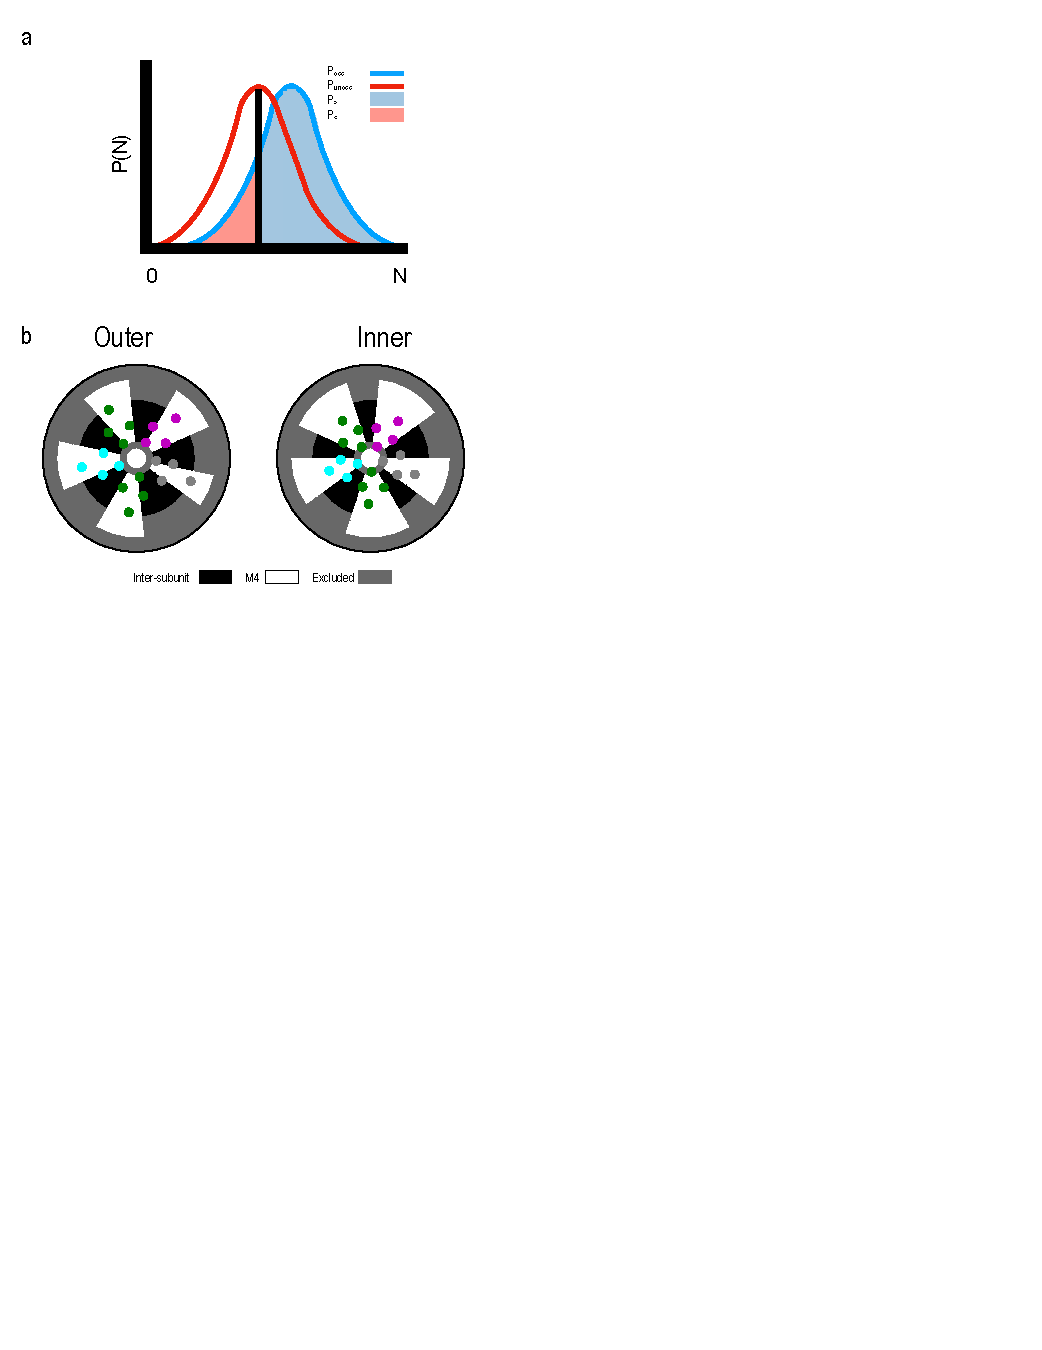
\includegraphics[width=\linewidth]{PartialBIndingToy.pdf}
	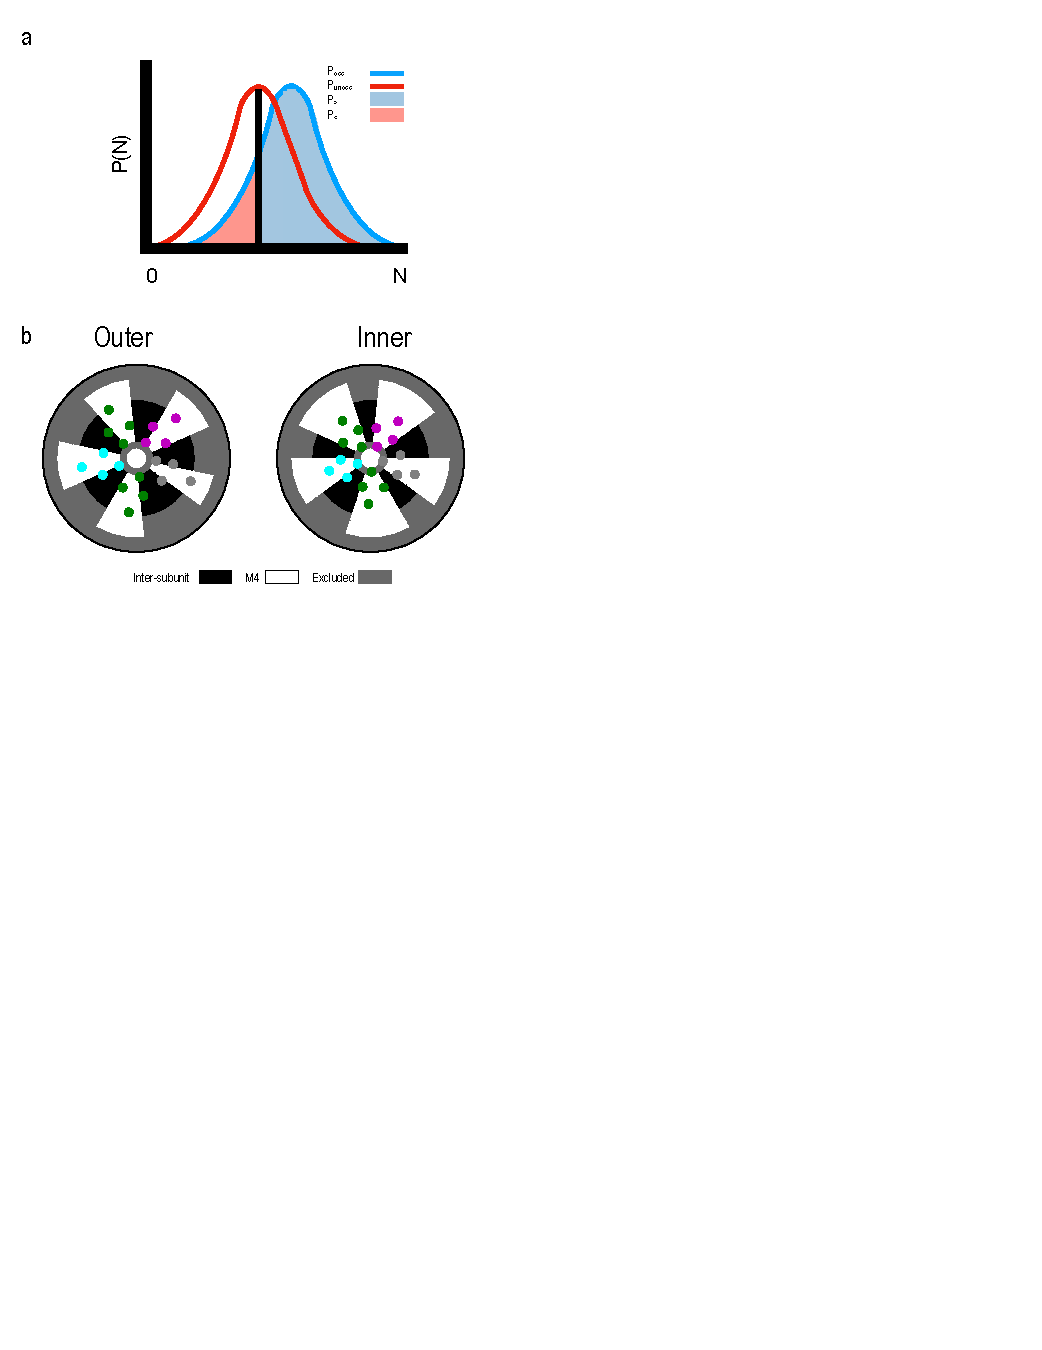
\includegraphics[width=\linewidth]{PartialBIndingToy.pdf}
	\caption{{ Binding site boundaries and distribution definitions.}  (a) Structure of the \nachr{} TMD\cite{Unwin2005}, viewed from the extracellular domain. Helices are colored by subunit ($\alpha$:green, $\beta$:purple, $\gamma$: cyan, $\delta$:grey). (b) Boundaries of the pseudo-symmetric \liam{inter-subunit} (black) and M4 (white) sites. The angular components are determined by the location of the M1 and M3 helices for either two adjacent subunits (\liam{inter-subunit} sites) or a single subunit (M4 sites), and are listed in Table S5. Circles correspond to the helices shown in panel A.  (c)  The distributions $P_{site} (n)$ (blue) and $P_{bulk}(n)$ (dashed red) represent the probability distributions for number of beads of a certain lipid species in the site or in an analogously-sized area of the bulk, respectively. The value $n_{peak}$ maximizes $P_{bulk}$. $P_<$ (pink) is the area under $P_{site}$ to the left of $n_{peak}$ while $P_>$ (light blue) is the area under $P_{site}$ to the right of $n_{peak}$. }
	\label{fig:PBT}
\end{figure*}

\subsection{Calculation of Polar Density Distributions}
As in our previous work\cite{Sharp2019, Woods2019, Tong2019}, the two-dimensional density distribution $\rho_{B}$ of the beads within a given lipid species $B$ around the protein was calculated on a polar grid:
  \begin{equation}
      \rho_{B}(r_i,\theta_j)= \frac{\left\langle n_{B}(r_i,\theta_j) \right\rangle}{r_i \Delta{r}\Delta{\theta}} \\        
    \label{eq:R}
  \end{equation}
  where  $r_i = i \Delta{r}$ is the projected distance of the bin center from the protein center, $\theta_j = j \Delta{\theta}$ is the polar angle associated with bin j,  $\Delta{r}$= 10\AA~ and  $\Delta{\theta} = \frac{\pi}{15}$ radians are the bin widths in the radial and angular direction respectively, and $\left\langle n_{B}(r_i,\theta_j) \right\rangle$ is the time-averaged number of beads of lipid species $B$ found within the bin centered around radius $r_{i}$ and polar angle $\theta_{j}$.  In order to determine enrichment or depletion, the normalized density $ \tilde{\rho}_{B}(r_i,\theta_j)$ is calculated by dividing by the approximate expected density of beads of lipid type B in a random mixture, $x_{B}s_{B}~N_{L}/\langle L^{2}\rangle$, \grace{where $x_{B}$ is the fraction of lipid B in the membrane}, $s_{B}$ is the number of beads in one lipid of species B, $N_{L}$ is the total number of lipids in the system, and $\langle L^{2}\rangle$ is the average projected box area:
  \begin{equation}
  \tilde{\rho}_{B}(r_i,\theta_j)=\frac{ \rho_{B}(r_i,\theta_j)}{x_{B}s_{B}~N_{L}/\langle L^{2}\rangle}. \\        
    \label{eq:Rt}
  \end{equation}
Python software for these calculations are under active development and are available online\cite{2Dgithub}.  
 
This expression is approximate because it does not correct for the protein footprint or any undulation-induced deviations of the membrane area.  The associated corrections are small compared to the membrane area and would shift the expected density for all species equally, without affecting the comparisons we perform here. For a given lipid species or class, analysis excluded any replicas in which fewer than 5 lipids of the species/class were in the leaflet at any point in the sampled simulation.
 %\grace{LMS:Previous sentence is woefully insufficient.  How did you get the distributions of the number of beads per site? (i.e. Was it a distribution across frames? Or across sites? How did you determine the number of beads in a site each frame? How frequently did you sample? } For the affinity calculation described above the bin radial and angular widths are $\Delta r=$  4$\AA$ and $\Delta \theta=$ $\frac{\pi}{25}$.\grace{LMS: I moved this sentence up here because the information fits here, but it needs to be adjusted to fit with this section}

 \subsection{Calculation of the \newaffinity}
 
Although lipids \liam{do occupy} clearly detectable hot-spots, binding to these sites are not straightforward to describe by a traditional two-state model. Lipids are chains that may partially occupy or fully occupy a site, and they may share a site with another lipid that is partly or fully occupying the site.  While the standard affinity can be determined from the probability of single occupancy, the \newaffinity{} is determined from the probability that a site is occupied by more beads than would be expected based on bulk density. %instead we consider partial occupation. Partial occupancy ranges from fully occupied, partially occupied, or unoccupied. A site is fully occupied if a single lipid species (A) is the only lipid species occupying a site. Like the small molecule displaced by water, a portion of lipid A may be partially or fully displaced by a second lipid (B). 

%A traditional affinity reflects the free energy difference between an occupied and unoccupied state, where we consider the free energy difference between enriched density in the site and depleted density in the site.  

For a given site, consider %Free energy calculations are defined as the change in the Gibbs' free energy ($\Delta G$). $\Delta G$ is calculated using 
two probability distributions: the probability $P_{site}(n)$ of finding $n$ beads within the site and the probability $P_{bulk}(n)$ of finding $n$ beads within a region of equivalent area \grace{in a randomly-mixed bulk}, respectively. For a lipid that has no affinity for this binding site, we expect $P_{site}(n) = P_{bulk}(n),$ while $P_{site}(n)$ should be right-shifted for a strong affinity and left-shifted in the presence of competition. %\grace{LMS please notice that I have changed $P_{occ}$ to $P_{site}$ because it contrasts better with $P_{bulk}$. This will need to be changed in any figures.} %Both distributions are calculated from the time averaged number of lipid beads within the area of an occupancy site ($P_{occ}$) or an identical area in the bulk membrane ($P_{bulk}$).  
We calculate the degree of right or left shift by first finding the number of beads $n_{peak}$ corresponding to the peak of the density distribution in the bulk.  \grace{ For a randomly-mixed bulk we expect $P_{site}(n)$ to be unimodal and close to Gaussian, so $n_{peak}$ should be approximately equal to the mean occupancy $\langle n\rangle$. Using the mode ($n_{peak}$) rather than $\langle n\rangle$ preserves the discretization of the original distribution and is less sensitive to extreme outliers. For a phase-separated bulk with a multimodal distribution, $\langle n\rangle$ would be more meaningful than $n_{peak}$. Alternatively, it would be possible to calculate a different affinity with respect to each reference phase,  by determining $n_{peak}$ using regions that are completely contained within specific phases. }

As illustrated in Figure \ref{fig:PBT} C, we then integrate $P_{site}$ on both the left and right side of the threshold $n_{peak}$ to yield $P_{<}$ and $P_{>}$ respectively:
\begin{eqnarray}
    %P_{<} \equiv \big\{\sum P_{occ} \leq \big< P_{bulk} \big> \big\} \label{eq:Pl} \\
    %P_{>} \equiv \big\{\sum P_{occ} > \big< P_{bulk} \big> \big\} \label{eq:Pg}
    P_{<}& \equiv &\sum\nolimits_{n\le n_{peak}} P_{site}(n) \label{eq:Pl} \\
    P_{>}& \equiv &\sum\nolimits_{n>n_{peak}} P_{site}(n)  \label{eq:Pg}
\end{eqnarray}
 \grace{While all probability distributions in the current manuscript are unimodal (\liam{Figure SI 1}), this approach is not limited to unimodal distributions of $P_{site}$. Regardless of the shape of the distribution for the bound state, the threshold separates it into two macrostates analogous to those in a classic binary binding model.}   %Using the mean value of $P_{bulk}$ ($ \big< P_{bulk} \big> $) as a reference, the sum of $P_{occ}$ less than or equal to   $\big< P_{bulk} \big> $ is defined as $P_{<}$. The sum of  $P_{occ}$ greater than  $\big< P_{bulk} \big> $ is defined as $P_{>}$. The affinity is then defined as the overlap between $P_{<}$ and $P_{>}$.
The free energy difference between the two macrostates is
\begin{equation}
\Delta G = -RT\ln\frac{P_{>}}{P_{<}}
\label{eq:dG}
\end{equation}
where R is the gas constant and T is temperature. We term this free energy difference the ``\newaffinity''.  In the special case of binary occupancy, 
\begin{eqnarray}
P_{site}(n)&= 
\begin{cases}
    (1+ K_{D}/[L])^{-1},& \text{if } n = 1\\
    (1+ [L]/K_{D})^{-1},& n=0
\end{cases}
\end{eqnarray}
where $K_{D}$ is the dissociation constant and $[L]$ is the ligand concentration. In a dilute solution the volume per ligand is typically much larger than the site volume, yielding $P_{bulk} (n)=1$ for $n=0$ and vanishes for all $n>0$, yielding $n_{peak} = 0$. Consequently, for this special case, $P_{<} = (1+ [L]/K_{D})^{-1}$ and $P_{>} = (1+ K_{D}/[L])^{-1}$. 
Then Equation \ref{eq:dG} reduces to the classic form for the chemical potential $RT\ln K_{D}-  RT\ln [L]$. 

\subsection{Binding Site Definition and Occupancy Calculations}

We consider four classes of site: each of the two leaflets contains a concave \liam{inter-subunit} site class and a convex M4 site class. There are five pseudosymmetric sites within each site class, for a total of twenty sites (Figure \ref{fig:PBT}B).  The boundaries for each site were drawn to correspond to the localized binding hot spots observed for heteroacidic membranes\cite{Woods2019}, and are non-overlapping. Inter-subunit sites include bins with angular components between the M1 and M3 helices of two adjacent subunits, and a radial component satisfying $10<r\leq32$\AA.  M4 sites include bins with complementary angular components (so that no sites overlap) falling within the M1 and M3 helices of a single subunit, and a radial component satisfying $10<r\leq44$\AA. For a full description of radial and angular dependencies, please see Table SI 4. 

In order to calculate $P_{site}(n)$, a distribution was taken across frames at 10 ns intervals. For any frame, the  beads of a given lipid or chain type were binned onto a fine polar grid with $\Delta r=$  \liam{4\AA~} and $\Delta \theta=$ $\frac{\pi}{25}$. The bins falling within the site boundaries were then summed to calculate the occupancy $n$.  This approach allowed for straightforward adjustment of site boundaries if needed without needing to re-bin the whole trajectory. \grace{All density-threshold affinities reported in the main manuscript reflect at least 290 samples with $n\ge 1$; most values represent at least 10,000 samples.  In the Tables SI 3.1-3.4, we provide a further breakdown of affinities by specific lipid species and pseudosymmetric sites, and these values may represent fewer samples.} 
 % Using the polar density distributions, we isolated specific sites with masks based on the above site limits. For each site, the number of beads of a specific lipid species (or acyl-chain species) were counted every 10$ns$ of the trajectory. %Probability distributions are the number of lipid beads within a given site over 
%Finer bins are required to accurately describe specific sites. Instead radial and angular widths are changed to: 

\subsection{Calculation of Accessible Area}

Calculation of $P_{bulk}$ requires determining the accessible site area in order to calculate the densities in a bulk region of similar area. The area $A$ accessible to the lipids is the difference between the total site area $A_{tot}$ and the area $A_{ex}$ excluded by the protein: $A = A_{tot} - A_{ex}$\liam{.} 
%We are interested in $A_{acc_s}$, which appears in eq \ref{eq:As}. 
$A_{tot}$ is straightforward to calculate by summing over the areas of the bins $i$ within the site boundaries: $A_{tot} = \sum_i r_i \Delta r_i  \Delta \theta_i$.  Calculating $A_{ex}$ is less straightforward, and although there are many possible ways to do this, for self-consistency we used the same tools from our primary analysis.  

In a single lipid membrane, $P_{site}(n)=P_{bulk}(n)$ as long as $P_{bulk}(n)$ is calculated using the proper area $A$.  We exploit this identity to calculate $A$ for each site, by running a single \nachr{} in pure di-palmitoyl phosphatidylcholine (DPPC) for \liam{$\sim 370$~ ns at 323 K} and determining the value of $A$ for each site such that $P_{site}(n)$ and $P_{bulk}(n)$ have the same peak.  These areas are reported in Table SI 4. 
%\begin{equation}
    %A_s = \frac{\left\langle n_s(r,\theta) \right\rangle}{\rho_s(r,\theta)}
%    A_tot = \sum_s r_s \Delta r_s  \Delta \theta_s
%\label{eq:A}
%\end{equation}
%where $\left\langle n_s(r,\theta) \right\rangle$ is the associated time averaged number of beads within a polar bin and $\rho_s$ is the time averaged numeric bin density (eq \ref{eq:R}). \grace{LMS: Why don't we just calculate the bulk area by summing the bin areas? Why do we divide n by rho? This seems really unnecessary.} \liam{Ah, yes, we do what you wrote. What I have is from like... may? } Only values of $\left\langle n_s(r,\theta) \right\rangle$ and  $\rho_s$ within the range of angular and radial bins described above are used. Using the values calculated for $A_s$, we calculate $A_{acc}$ to determine accurate bulk densities for $P_{bulk}$.

%    \begin{equation}
 %   	A_{acc_s} \equiv \frac{\left\langle n_{site_s} \right\rangle A_s }{\left\langle n_s \right\rangle} \label{eq:aac}\\
 %   \end{equation}
    
%    \begin{equation}
 %   	A_{rest_s} \equiv A_s - A_{acc_s} \label{eq:aac}\\
 %   \end{equation}
    
%    $\left\langle n_{site_s}\right\rangle$ and $\left\langle n_s  \right\rangle$ are the average number of lipid beads for a specific occupancy site and the average number of lipid beads in the bulk membrane within a given area $A_s$. The values for $A_{acc_s}$ are then used to calculate $P_{bulk}$, see Figure \ref{fig:PBT} a.
%    \grace{This piece confuses me and I need to understand it better before I can edit.} \liam{I think I should have also had $A_{rest}$, this is to show how we determine the accessible and restricted areas.}

 \begin{figure*}
	\center
	\includegraphics[width=\linewidth]{Trajectory.pdf}
	%\includegraphics[width=3in]{Trajectory.pdf}
	\caption{{A molecular perspective of coarse-grained simulation results}. a) Multiple frames from a single simulation replica over 5 $\mu s$.   The \nachr{} TMD is shown in surface representation and colored as in Figure 1. Cholesterol and acyl chains within 15 \AA~ of \nachr{} are shown as beads, and colored by chain type: saturated lipids: blue, monounsaturated lipids:orange, n-6 PUFAs:pink, n-3 PUFAs: beige, and cholesterol: red.  Each phospholipid color includes several lipid species of the same type, and simulations included a larger membrane and the ECD, which is not shown.  b) Representative poses of lipids for individual sites, colored as in A, but viewed from within the membrane looking at the TMD surface. \grace{The labeled chain is opaque, while the rest of the lipid is translucent.} Cholesterol selects for the \liam{inter-subunit} site while monounsaturated lipids have a particularly low affinity for this site. PUFAs select for the M4 site, while saturated lipids have a particularly low affinity. }
	\label{fig:trj}
\end{figure*}

\section{Results and Discussion}
\label{res}

\begin{figure*}[!h]
	\center
	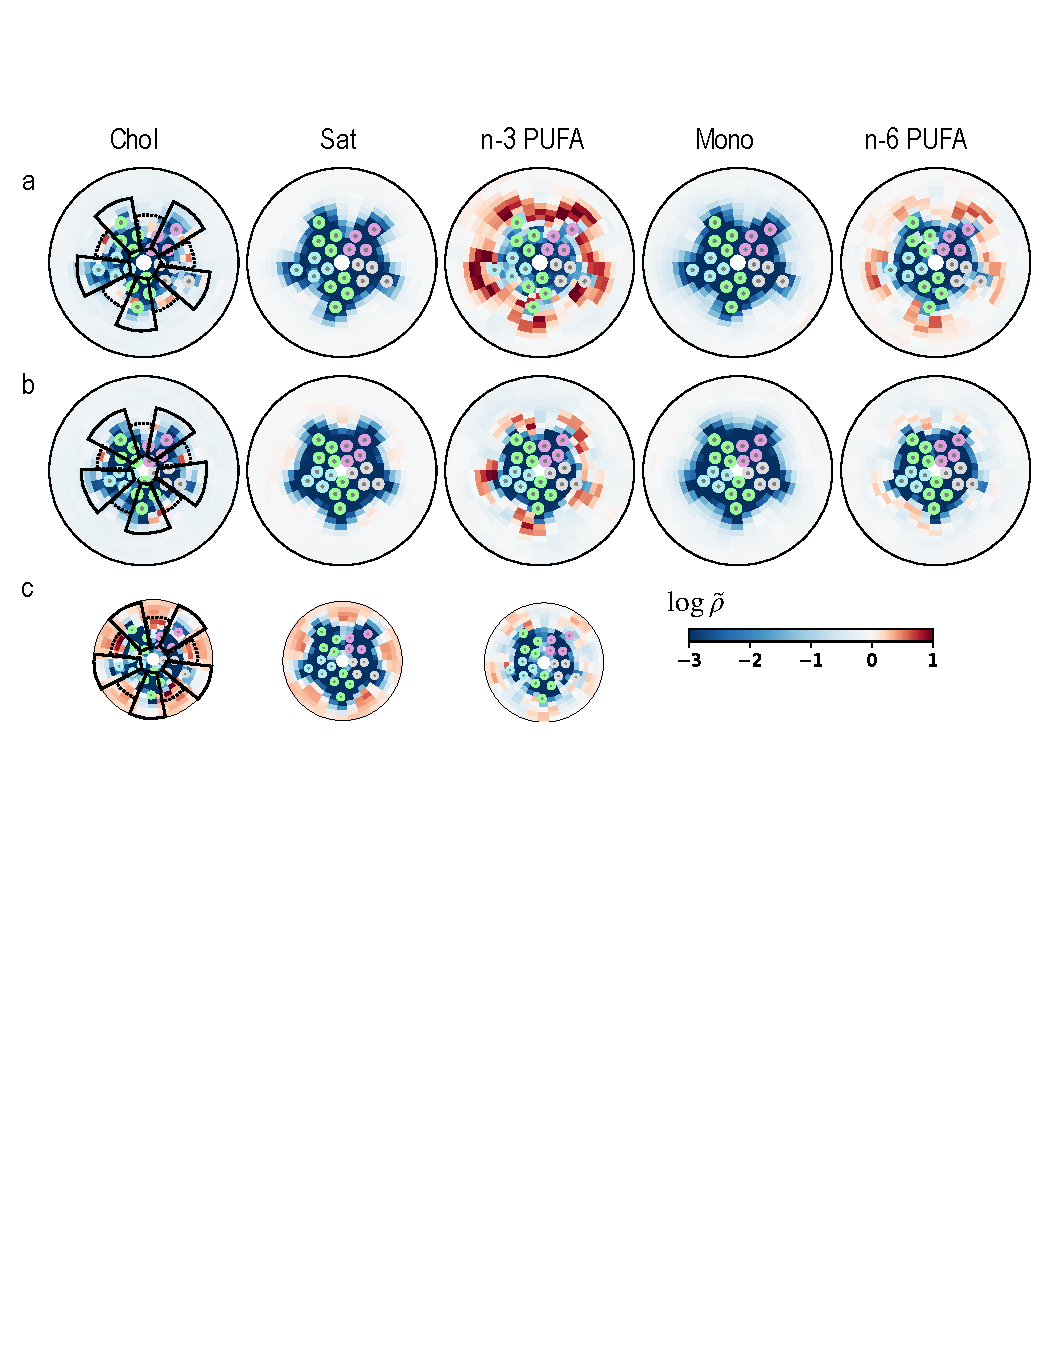
\includegraphics[width=\linewidth]{acyl_heatmap.pdf}
	%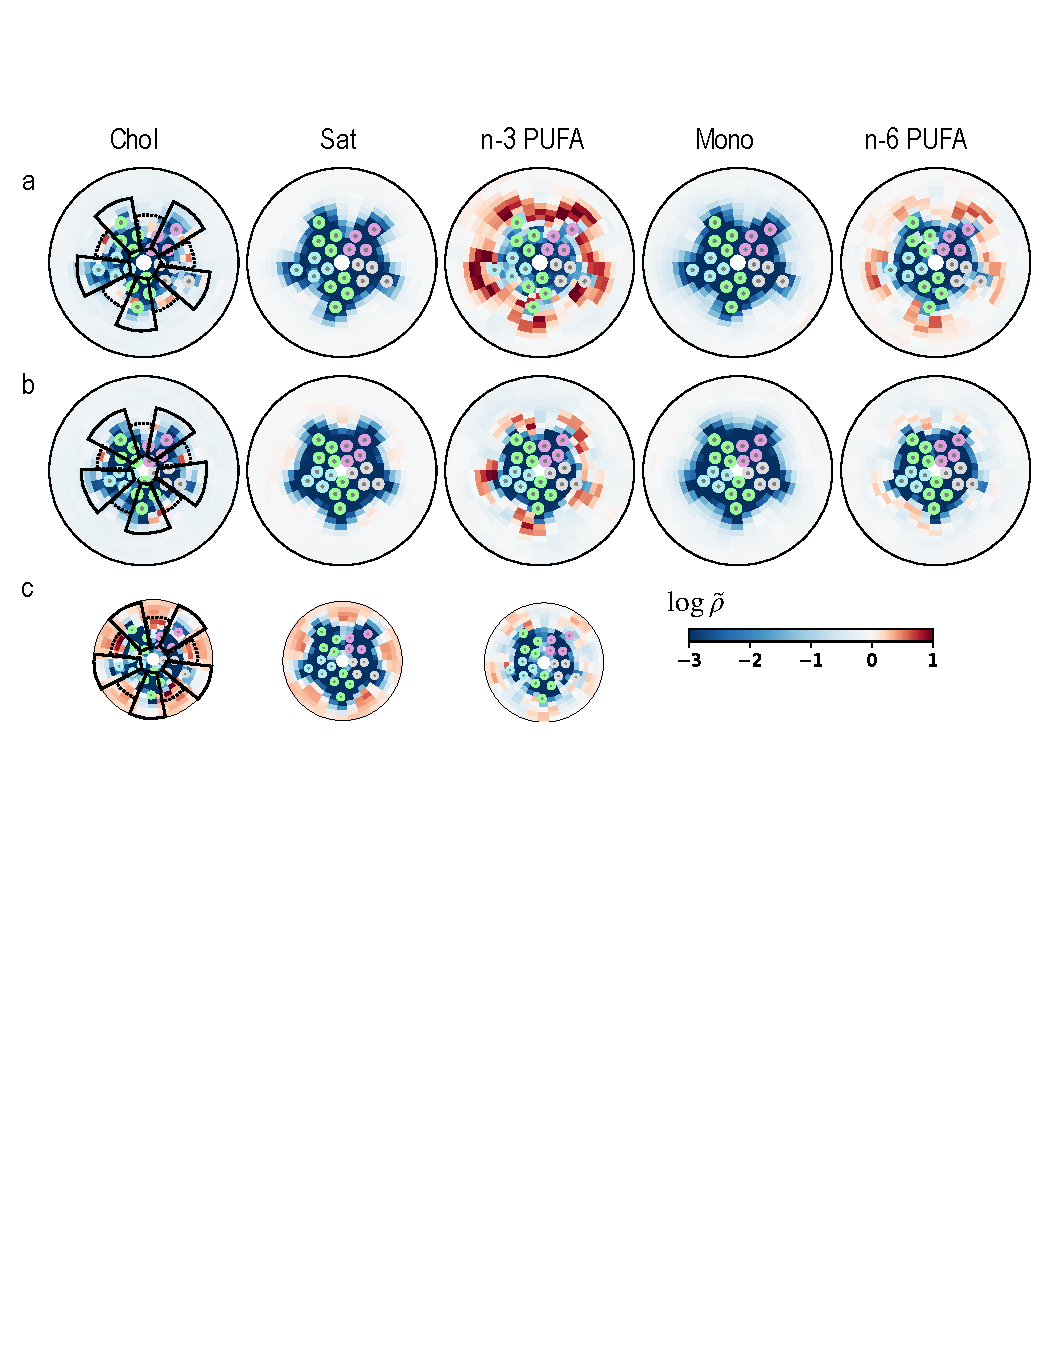
\includegraphics[width=\linewidth]{acyl_heatmap.pdf}
	%55mm]{acyl_heatmap.pdf}
	\caption{{Lipid density enrichment around a central singular \nachr.} Density enrichment $\tilde{\rho}$, calculated using eq \ref{eq:Rt}, for lipids in a neuronal (a-b) and model (c) membrane.  Depletion relative to a random mixture ($\log\tilde{\rho}< 0$) is blue while enrichment ($\log\tilde{\rho}> 0$) is red. Acyl chain density includes only the relevant chain of a heteroacidic lipid, while cholesterol density includes the whole cholesterol molecule.  Helices are represented as circles colored as in Figure 1. Cholesterol density maps also show boundaries of inter-subunit and M4 sites, as in Figure \ref{fig:PBT}b. The maximum radius from the \nachr{} pore is 60 \AA. (a) Enrichment within the outer leaflet of a neuronal membrane. \grace{Each average represents 25 $\mu$s of total sampling across ten replicas, each of which contributes 2.5$\mu$s of data collected after 2.5 $\mu$s of discarded equilibration.} (b) As in (a), but for the inner leaflet. (c) Equivalent analysis for the outer leaflet of \nachr{} in a symmetric model membrane of 2:2:1 n-3 PUFA:saturated:cholesterol, using previously published trajectories\cite{Woods2019}.} 
	 %describes acyl-chain depletion compared to a random bulk mixture, $\tilde{\rho}_{a}=0$ describes the expected mixture, and $\tilde{\rho}_{a}  > 1$ describes acyl-chain enrichment compared to a random mixture. a) Density enrichment based on acyl-chains, b) density enrichment based on head group charge.}
	\label{fig:acyl_map}
\end{figure*}


\begin{figure*}[!h]
	\center
	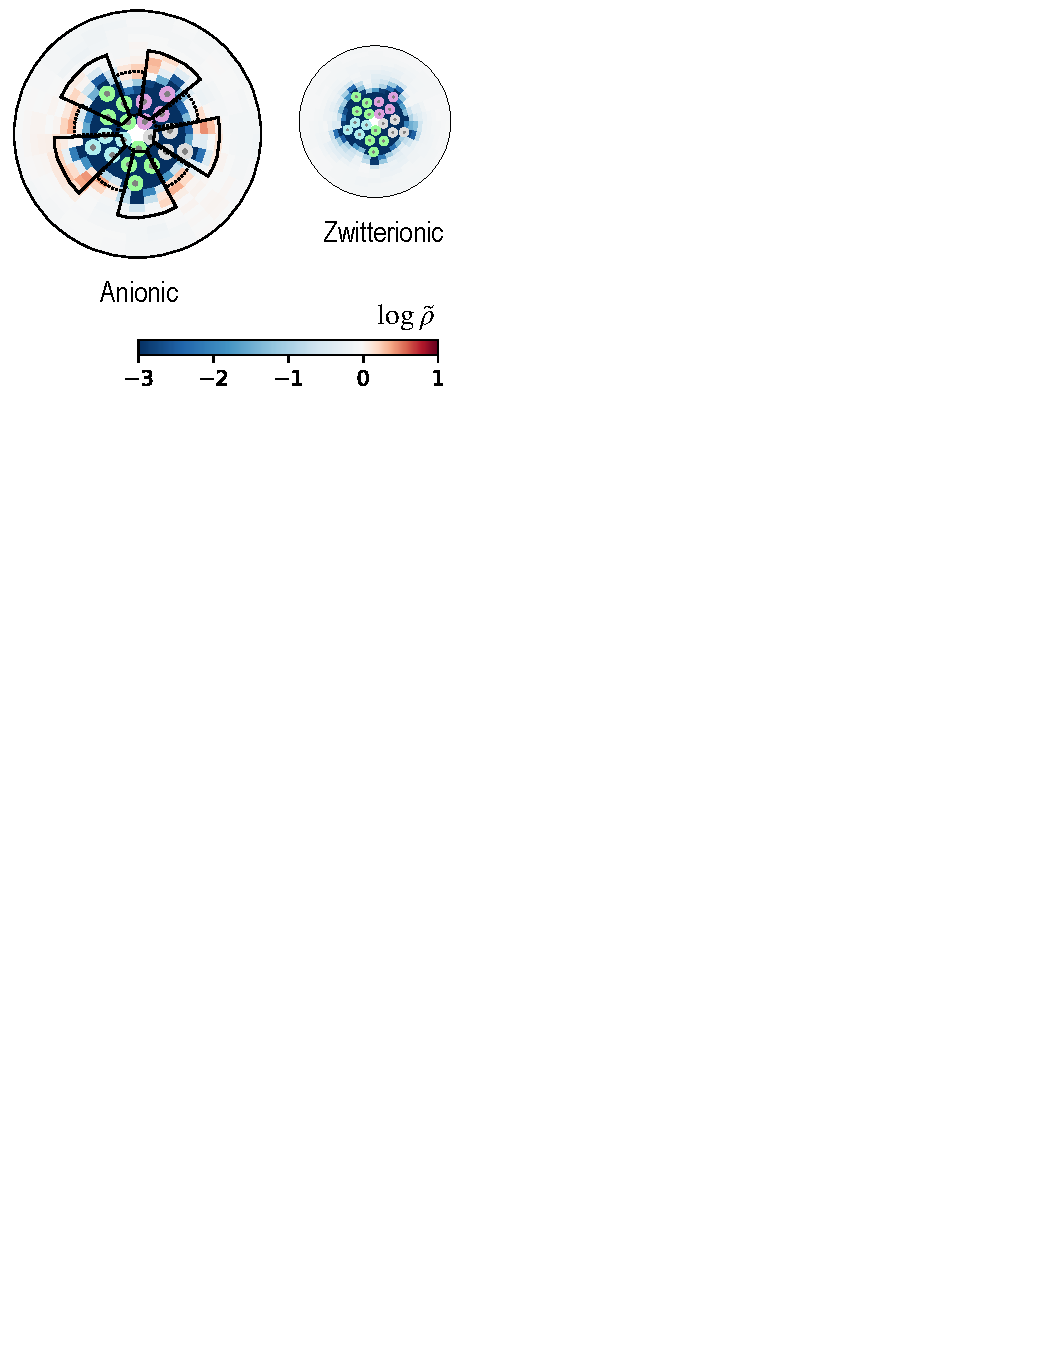
\includegraphics[width=0.5\textwidth]{ChargedHG_heatmap.pdf}
	%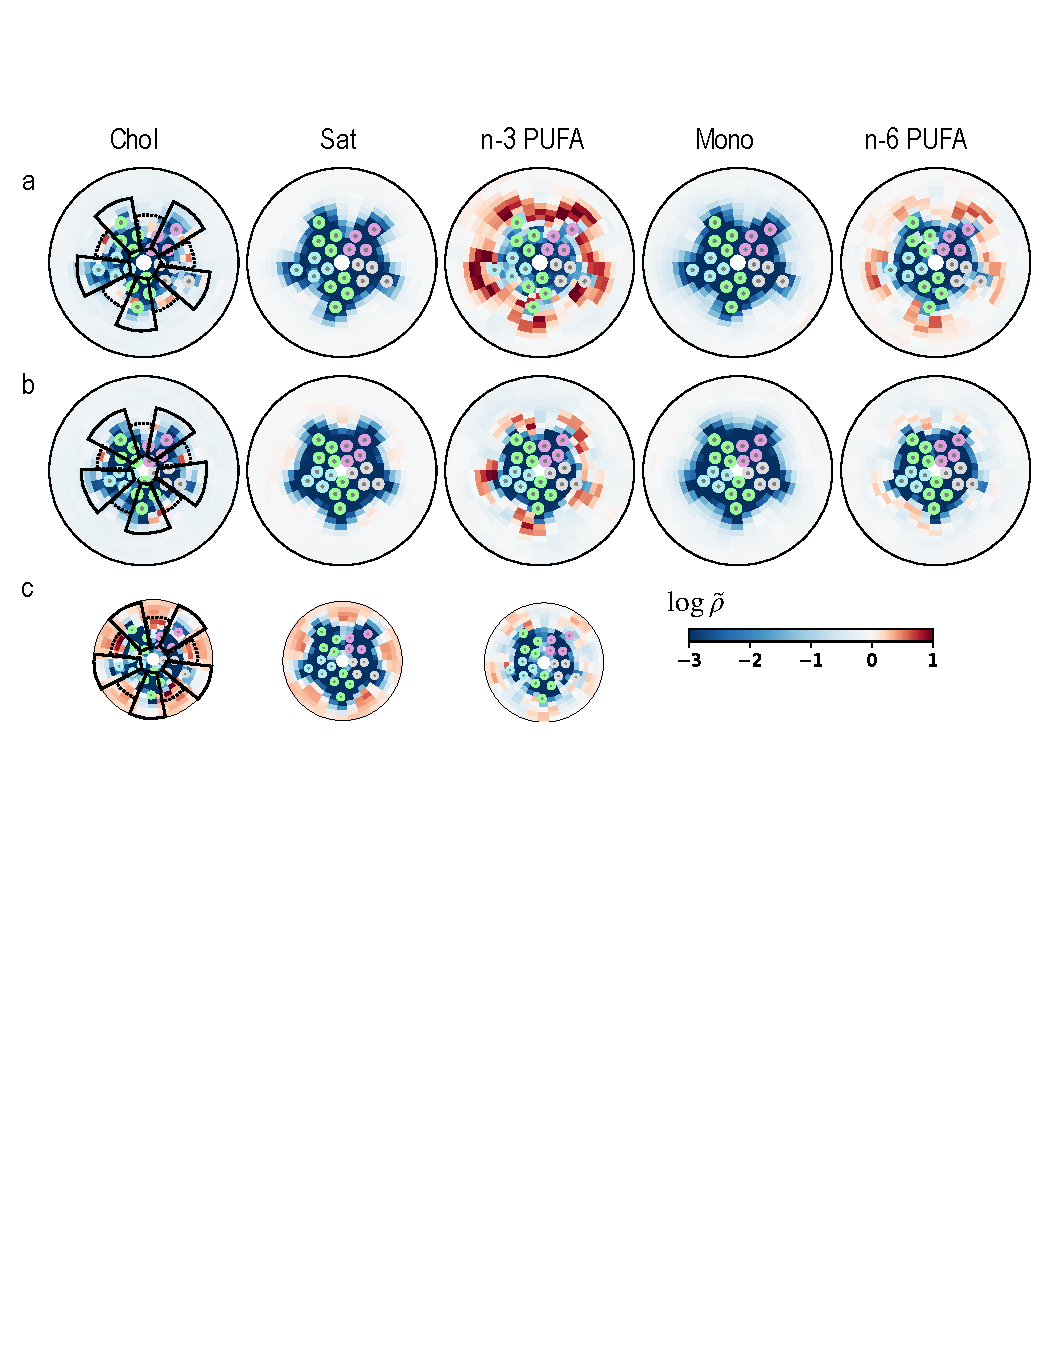
\includegraphics[width=\linewidth]{acyl_heatmap.pdf}
	%55mm]{acyl_heatmap.pdf}
	\caption{{Enrichment around of charged lipids in the inner leaflet around a central singular \nachr.}  Density enrichment $\tilde{\rho}$ for anionic (left) or zwitterionic (right) phospholipids in a neuronal membrane, calculated using eq \ref{eq:Rt} for the inner leaflet. Each average represents 25 $\mu$s of total sampling across ten replicas, each of which contributes 2.5$\mu$s of data collected after 2.5 $\mu$s of discarded equilibration. The maximum radius from the \nachr{} pore is 60 \AA. Depletion relative to a random mixture ($\log\tilde{\rho}< 0$) is blue while enrichment ($\log\tilde{\rho}> 0$) is red. Density includes the whole lipid.  Helices are represented as circles colored as in Figure 1. } 
	 %describes acyl-chain depletion compared to a random bulk mixture, $\tilde{\rho}_{a}=0$ describes the expected mixture, and $\tilde{\rho}_{a}  > 1$ describes acyl-chain enrichment compared to a random mixture. a) Density enrichment based on acyl-chains, b) density enrichment based on head group charge.}
	\label{fig:charge_map}
\end{figure*}

\subsection{Effect of acyl chain on site selectivity among neutral lipids}

%\textit{SECTION 3.1:  EFFECT OF ACYL CHAIN ON NEUTRAL LIPID AFFINITIES a) Results block for figure 2.  b) Results block for figure 3 (neutral)  c) Results block for figure 4 (neutral). Results blocks in all three cases should be focused on role of unsaturation/chain flexibility.}

%Results from Woods et al 2019 \cite{Woods2019} predict lipid occupancy sites for PUFAs and raft forming lipids at M4 and inter-subunit sites respectively. To test this whether we observe similar behavior in neuronal membranes, we use radial enrichment densities (see eq \ref{eq:Rt}) and calculated affinities as $\Delta G$ values, described in methods and equations \ref{eq:A}-\ref{eq:dG}.

\begin{figure*}[!h]
	\center
	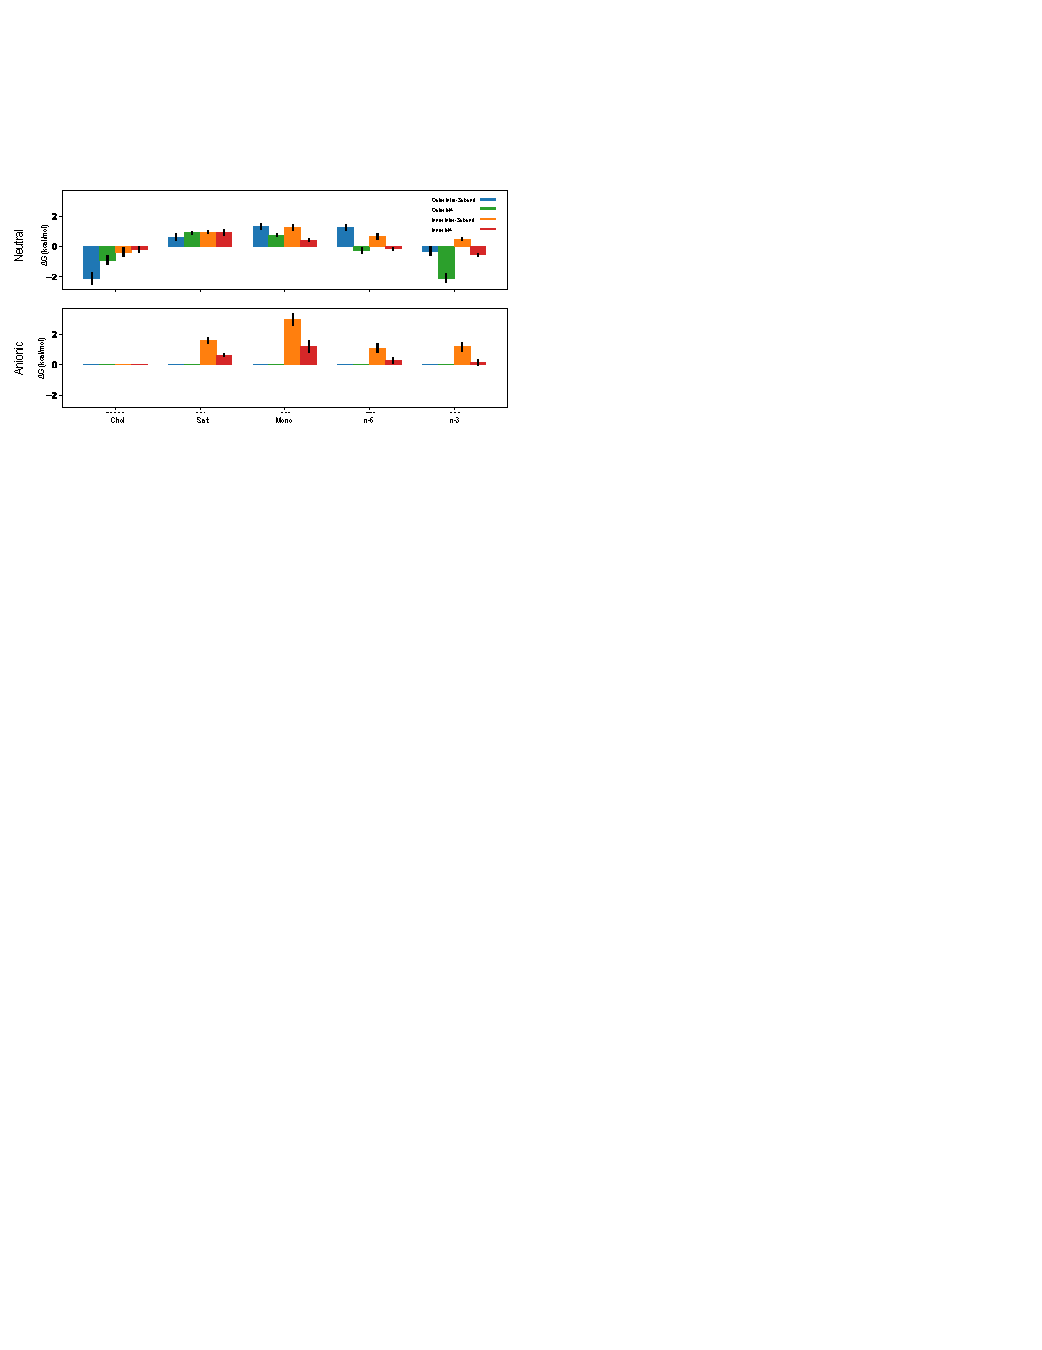
\includegraphics[width=\linewidth]{Protein_centric.pdf}
	\caption{{\Newaffinities{} organized to reveal site selectivity.} The \newaffinities{} ($\Delta G$) are calculated using Equation \ref{eq:dG}, where error bars are the standard error (n=10 independent replicas).  \Newaffinities{} are colored by site; in the outer leaflet:  \liam{inter-subunit} (blue) and  M4 (green), and for the inner leaflet: \liam{inter-subunit} (orange) and M4 (red). Values are separated by headgroup charge (rows) and acyl chain type (columns). More negative values indicate stronger affinities, while more positive values indicate more displacement of the lipid by other lipid species. Data incorporates 10 replicas averaging over the last half of the 5$us$ trajectory, with five-fold averaging over each type of pseudosymmetric site. Figure \ref{fig:lipidBar} has an alternate representation of the same data.  }  % Colors: Outer Inter-Subunit:blue, Outer M4:green, Inner Inter-Subunit:orange, Inner M4:red.}
	\label{fig:proBar}
\end{figure*}

Representative frames from a typical trajectory of boundary lipids are shown in Figure \ref{fig:trj}A, with representative poses shown in Figure \ref{fig:trj}B.  In order to quantitatively compare the lipid distributions for the native system to our previous model system, we plotted the enrichment of boundary density relative to bulk density on a two-dimensional polar heat map centered around the protein. This enrichment is shown in Figure \ref{fig:acyl_map}A for cholesterol and various acyl chains grouped by  saturation. Saturated and monounsaturated acyl chains are not significantly depleted or enriched in the boundary of the protein. Regions of cholesterol density are much more localized than in the model membrane (Figure \ref{fig:acyl_map}C), with pockets of high enrichment very close to the protein and weak depletion in the remainder of the boundary region.  Both n-6 and n-3 PUFA chains yield five-fold symmetric enrichment around the M4 \liam{helices}, as observed for n-3 PUFAs in the model membrane.  In the neuronal membrane, however, this enrichment is less well-defined and spreads into the inter-subunit regions. In particular, additional pockets of significant enrichment are apparent in the $\beta-\delta$ subunit interface in the outer leaflet. The overall area of the regions of PUFA-enrichment decrease in the inner leaflet, where n-3 PUFAs are enriched around M4 \liam{helices}, but n-6 PUFA density is not five-fold symmetric and has weak enrichment. Overall, the loss of definition in site boundaries diverges from the well-defined five fold enrichment for n-3 PUFAs we saw in model membranes\cite{Woods2019}. 

In order to reduce these distributions to affinities that are more straightforward to interpret, we calculated the \newaffinity{}  $\Delta G$ for various lipid species as defined in Eq. \ref{eq:dG}. We organize this information in two different ways: Figure \ref{fig:proBar} provides the ``lipid's perspective'' and is organized to identify the preferred site for a given lipid type (the lipids' ``site selectivity''), while Figure \ref{fig:lipidBar} provides the ``site's perspective'' and is organized to identify the most favorable lipids for a given site (the sites' ``lipid specificity''). 

We first consider site selectivity for neutral lipids. Affinities for neutral lipids and cholesterol are shown in Figure \ref{fig:proBar}A, where more negative values of $\Delta G$ indicate a stronger \newaffinity{} and more positive values indicate more displacement by other lipids.  Overall, as shown in Figure \ref{fig:proBar}A, saturated lipids have similar \newaffinities{} across all sites, which is consistent with the generally flat distribution observed in Figure \ref{fig:acyl_map}. Yet saturated lipids do yield a slightly stronger affinity for  \liam{inter-subunit} sites, at least in the outer leaflet, which may drive the high amount of saturated enrichment observed at these sites in model membranes.  Outer leaflet monounsaturated lipids are slightly more unfavorable in  \liam{inter-subunit} sites than M4 sites, and this difference grows in the inner leaflet. 

In contrast to saturated and monounsaturated lipids, PUFAs and cholesterol are highly selective for particular site classes.  As shown in Figure  \ref{fig:proBar}A, neutral PUFAs have significantly stronger affinities for M4 sites than for innersubunit sites in the same leaflet.  Such selectivity is consistent with the PUFA enrichment density in Figure \ref{fig:acyl_map}A, where n-3 PUFAs can occupy most regions of the TMD but have particularly high levels of enrichment around M4. It is further consistent with our expectations from model membranes (Figure \ref{fig:acyl_map}C). Regardless of the site class, PUFAs favor the outer leaflet site over the inner leaflet site, but both sets of M4 sites are more favorable than both sets of inter-subunit sites.  Conversely, cholesterol has significantly stronger affinities for innersubunit sites than for M4 sites, which is also consistent with the enrichment density in Figure \ref{fig:acyl_map}A and our expectations from model membranes (Figure \ref{fig:acyl_map}C). For cholesterol, however, the leaflet is a bigger determinant of affinity than the site; cholesterol has a stronger affinity for either outer leaflet site compared to either inner leaflet site.  

\subsection{Lipid preferences of  \liam{inter-subunit} and M4 sites}
We now switch perspectives to considering which neutral lipids are most favorable for particular sites. As shown in Figure \ref{fig:lipidBar} A and B, inter-subunit sites in both leaflets prefer cholesterol to phospholipids, which is expected based on the results from model membranes.  Upon visual inspection, this result may appear to diverge from the cholesterol polar density plots in neuronal membranes (Figure \ref{fig:acyl_map} A).  The present results show that while the overall footprint of cholesterol enrichment in Figure \ref{fig:acyl_map} A is small, this small region actually reflects a tight and persistently occupied binding site.  The highly right-shifted distributions for cholesterol are shown in Figure S1.  %\grace{LMS: I'm not sure about the following explanation.  Did we discuss this? If so, can we discuss it again? } \liam{we had, though it was my understanding it was roughly the same as what is in the previous sentence.}    We argue difference between weak cholesterol enrichment and strong cholesterol affinity is a result of averaging. For the density analysis, the peak of the the lipid distribution is isolated as a result of averaging, while for the affinity calculation, the full distribution is used to compute the affinity, see Figure SI 1.

PUFA chains yield affinities for the  \liam{inter-subunit} site that are approximately $>$0.5 kcal/mol stronger than saturated lipid affinities (Figure \ref{fig:lipidBar} A and B), which was unexpected based on results from model membranes but is consistent with the corresponding enrichment density in Figure \ref{fig:acyl_map}A. More generally, neutral phospholipid affinities for  \liam{inter-subunit} sites obey the following trend, from strongest to weakest: n-3 $>$ n-6 $>$ saturated $>$ monounsaturated. Thus, even though PUFA chains prefer M4 sites to inter-subunit sites,  and saturated chains prefer inter-subunit sites to M4 sites, PUFAs have a stronger affinity for either site type than do saturated lipids. 
 
For  \liam{inter-subunit} sites, monounsaturated lipids have the weakest affinities ($>0.5$ kcal/mol), which may reflect a limited number of ways to pack the single kink of a monounsaturated chain in this concave site. In contrast, cholesterol and PUFAs are either small or highly flexible and may more easily pack across multiple sites. Saturated chains may pack parallel to the protein surface in these sites (Figure \ref{fig:trj}B) 
% may pack around inter-subunit site's concave topology. The single acyl-chain kink found in monounsaturated lipids may prevent packing of itself around inter-subunit sites, and is not flexible to compete with PUFA's occupying M4 sites. 

As shown in Figure \ref{fig:lipidBar}C and D, M4 sites in both leaflets have the strongest affinity for n-3 PUFAs, and affinity weakens as acyl chain rigidity increases; from strongest to weakest the phospholipid affinities follow: n-3 $>$ n-6 $>$ monounsaturated $>$ saturated.  This is consistent with a role for PUFAs in minimizing unfavorable membrane deformations caused by the \plgic's conical-star shape.\cite{Brannigan2007,Kim1998,Dan1993,Goulian1996,Goulian1993,Fournier2015}  Surprisingly, cholesterol had a stronger affinity for M4 sites than any acyl chains other than n-3 PUFAs. Cholesterol is rigid, small, and has asymmetric sides (rough and smooth) which potentially allows it to embed between \liam{helices} and compete with n-3 PUFAs for binding. Any cholesterol bound within the grooves of the subunit interface (as hypothesized based on atomistic simulations\cite{Brannigan2008} and observed in $\beta$ subunits  of \nachr{} using coarse-grained simulations\cite{Sharp2019}), will also get counted within the M4 site.   %Cholesterol's favorability for M4 is a result of its size and asymmetric shape, making it ideal for packing between alpha-helices. 

\grace{All pLGICs display a high degree of structural conservation in the TMD and ECD, both across proteins and across subunits of the same protein, but sequences can vary significantly. Affinities for each of the five-fold pseudosymmetric sites within each site class are given in Table SI 3.1-3.4, along with significance tests. Cholesterol selects for specific subunits within each of the site classes, which is consistent with its rigid structure. Three of the four site classes (intersubunit sites in both leaflets and outer leaflet M4 sites) include deep grooves in the protein, which could contribute to sequence-dependent affinities. Saturated, n-3, and n-6 chains reveal significant preferences within these site classes. Affinities for individual lipid species have a higher sampling error than aggregates based on headgroup or chain saturation, and most variations at the species level do not reach statistical significance. PUPE (a PE headgroup with one saturated chain and one long-chain n-3 polyunsaturated chain) is an exception; it reveals selectivity among all three grooved site classes.}

%Unlike phospholipids, cholesterol has the strongest affinity for inter-subunit sites, however cholesterol has affinity values $<0$ kcal/mol at all sites. 
%Figure \ref{fig:lipidBar} shows site affinity for acyl-species, and is sorted by charge and leaflet. Inter-subunit sites in both leaflets has the strongest affinity for cholesterol. 
%M4 sites in both leaflets have the strongest affinity for n-3 PUFAs. Both sites have distinct trends shared across leaflets. Inter-subunit sites have the phospholipid affinity trend: n-3 $<$ n-6 $<$ saturated $<$ monounsaturated, while 
%Cholesterol has the strongest affinity of the neutral lipids at inter-subunit sites for both leaflets, but inner inter-subunit sites affinity is $\sim 50 \%$ weaker. Neutral phospholipids at inter-subunit affinity values change $<0.5$ kcal/mol between leaflets.  Inter-subunit and M4 have different affinities trends: and  respectively. 
 %At the M4 sites, n-3 PUFAs interact more favorably than other lipids 
%\subsubsection{Discussion}
%Of the neutral lipids, n-3 PUFAs and cholesterol stand out. We predict the relative high affinity for n-3 PUFAs are a result of their flexibility. The n-3 PUFA, DHA, has several of unique membrane properties \cite{Stillwell2003a,Gawrisch2003}, and is observed to consistently interact with non-annular sites in and around \plgic s \cite{Sharp2019, Woods2019}. 


\begin{figure*}[!h]
	\center
	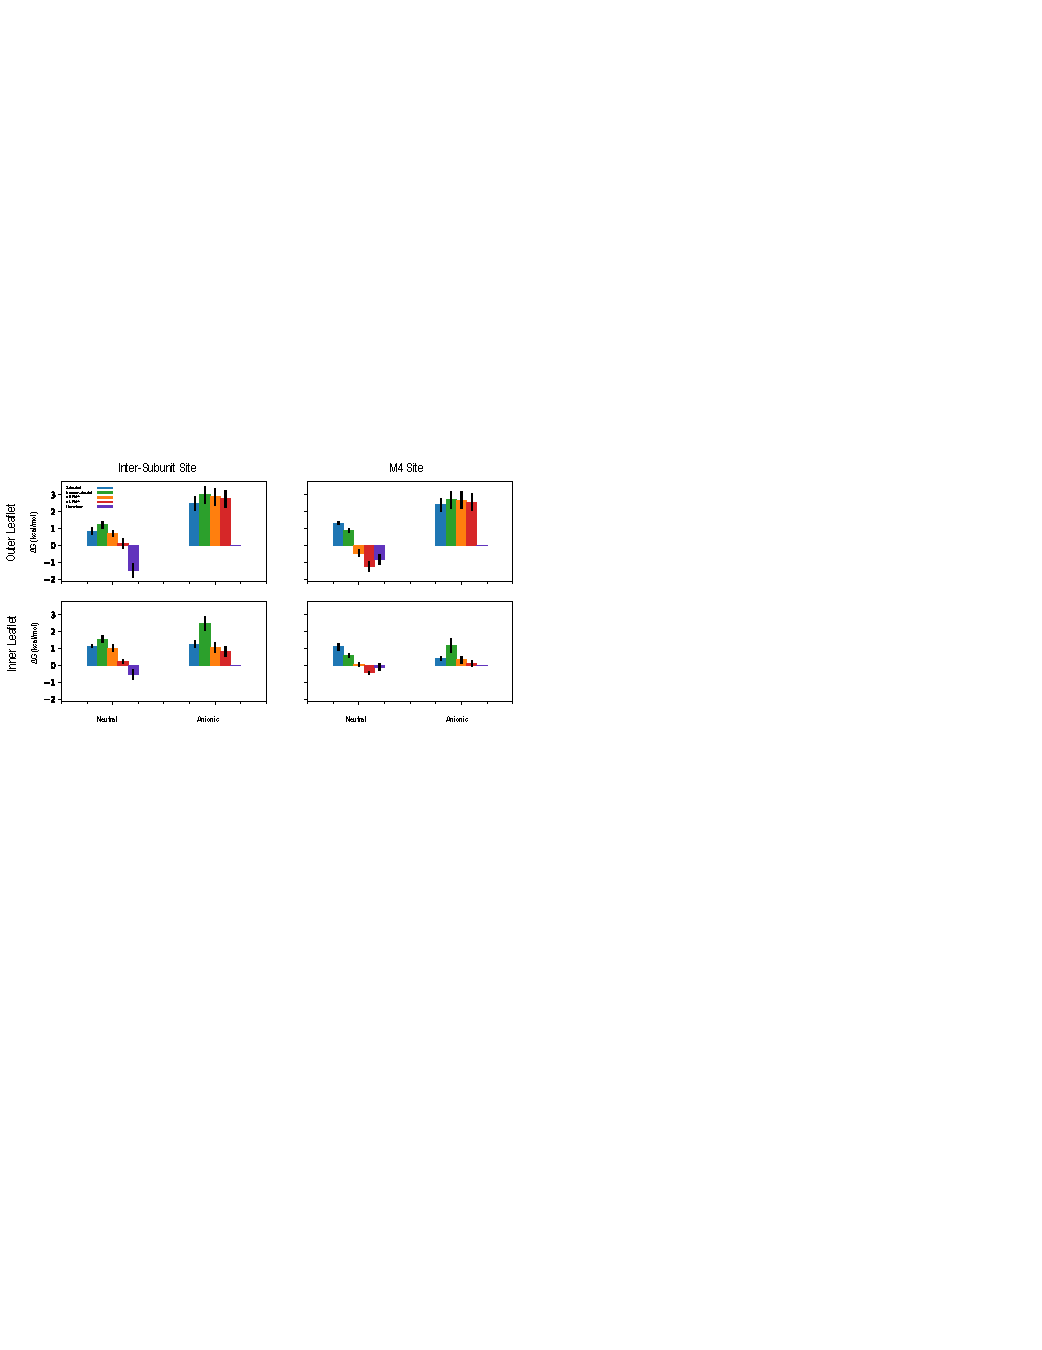
\includegraphics[width=\linewidth]{Lipid_centric.pdf}
	\caption{{\Newaffinities{} organized to reveal lipid preferences by site.} Data shown is identical but reorganized and recolored from Figure \ref{fig:proBar}. Here, \newaffinities{} are colored by chain type (Saturated:blue, Monounsaturated:pink, n-6 PUFAs:orange, n-3 PUFAs:tan, Cholesterol:red), and separated by leaflet (rows) and site (columns).} %More negative values indicate stronger affinities, while more positive values indicate more displacement of the lipid by other lipid species. Data incorporates 10 replicas averaging over the last half of the 5$us$ trajectory, with five-fold averaging over each type of pseudosymmetric site. } {Affinity calculation ranking for neutral and anionic lipid saturation species averaged the final 2.5 $\mu s$ simulations for each 10 replicas by occupancy site. Occupancy sites are averaged from 5 sites.\grace{LMS:Isn't it five sites?} Row one is the outer leaflet and row two is the inner leaflet. Columns are charge, each subplot is a difference occupancy site.  Error bars are the standard error calculated over the 10 replicas simulated. The smaller the number the stronger the affinity. Colors: Saturated:blue, Monounsaturated:green, n-6 PUFAs:orange, n-3 PUFAs:red, Cholesterol:purple}
	\label{fig:lipidBar}
\end{figure*}

\subsection{Effect of Head Group Charge on Affinity Depends on Leaflet and Binding Site}
%Research by Tong et al 2019 \cite{Tong2019} showed anionic lipids favorably occupied around arginines in ELIC's inner inter-subunit site. We hypothesize \nachr's outer TMD and inner inter-subunit sites will have a strong affinity for neutral phospholipids and \nachr's inner M4 sites will have a strong affinity for anionic phospholipids because M4 has more cationic amino acids, see Figure \ref{fig:aaa}a. We test the proposed lipid distributions using both enrichment density analysis and affinity calculations.
Figure \ref{fig:acyl_map}B compares the density enrichment for anionic headgroups with that of neutral headgroups. Data is shown for the inner leaflet only, because anionic lipids are not present in the outer leaflet at the start of simulations and few anionic lipids flip flop to the outer leaflet.% Furthermore, as shown in Figure \ref{fig:lipidBar}C, the anionic lipids that do flip in to the outer leaflet (\grace{LMS: how many is this?}) \liam{I'm not sure. Versions of the manuscript have had comments trying to bring up anionic distributions and affinities with you previously. It looks like 1 - 5 lipids flip? }  have very weak affinity for any sites in the outer leaflet ($\geq 2.0$ kcal/mol). These results are consistent with our previous observations that POPG had very weak affinity for the outer leaflet sites of ELIC\cite{Tong2019}.

In the inner leaflet, the anionic lipids are expected to select for sites that are lined with basic amino acids, which are in different locations depending on subunit (\liam{Figure SI 2})  As shown in Figure \ref{fig:charge_map}, anionic lipids are generally enriched around the M3/M4 \liam{helices} for the $\alpha_{\gamma}, \gamma,\delta,$ and $\beta$ subunits.  Anionic lipids are enriched at inter-subunit sites and around M4 sites for all subunits but the $\alpha$ subunits. Non-$\alpha$ \nachr~ subunits have basic amino acids closer to M4 \liam{helices}, as shown in \liam{Figure SI 2A}.  We incorporate data from all five pseudo-symmetric sites to obtain the \newaffinities{} reported in Figure \ref{fig:proBar}B, which suggest that anionic lipids have significantly stronger affinities for M4 sites on average. The average anionic affinity difference between inter-subunit and M4 sites is $\sim -1.0$ kcal/mol, as shown in Figures \ref{fig:proBar}, \ref{fig:lipidBar}D and SI Table 2. Although the magnitude of the affinity difference varies with acyl chain saturation, the sign is unchanged.     %Neutral lipids have weak enrichment around M4 sites in the outer leaflet, but other wise are neutral.
%We hypothesize the difference in our result is from the number and placement of charged amino acids in ELIC's (TMD PDB:3RQW\cite{Pan2012}) versus that of neuromuscular \nachr. We use VMD \cite{HUMP96} to visualize the difference between \nachr~and ELIC's inner \notsure{leaflet} TMD, . Both pLGICs have a number of cationic amino acids around their annulus. ELIC has more cationic amino acids embedded in the protein density than at the annulus. \notsure{Cationic amino acids found in the \nachr~structure tend to be more outward facing than cationic amino acids in the ELIC structure.} Non-$\alpha$ \nachr~ subunits have cationic amino acids closer to M4 alpha-helices. ELIC has cationic amino acids closer to the inter-subunit sites. Anionic amino acids are found at \nachr M4 alpha-helices, with the exception of the $\beta$ subunit. Anionic amino acids are found closer to the M1/M4 alpha-helices interfaces in ELIC, or embedded within the \liam{inner/non-annular/bulk of} protein.
%At inter-subunit sites the same trend with acyl-chain persists: n-3 PUFAs $>$ n-6 PUFAs $>$ saturated $>$ monounsaturated.  %In the outer leaflet, \nachr~ has preferential binding with cholesterol, neutral PUFAs, and then monounsaturated or saturated, the later are dependent on site.  
We now switch again to the ``site perspective'' to compare whether inner leaflet sites would prefer occupancy by anionic or neutral lipids. % compare the affinity of anionic lipids for inter-subunit sites the lower leaflet, see Figure \ref{fig:lipidBar}b. 
As shown in Figure \ref{fig:lipidBar}C, lipid affinity values for inter-subunit sites are either insensitive to charge (saturated or n-6 PUFA chains) or weaker for anionic lipids by at least 0.5 kcal/mol (monounsaturated and n-3 PUFA chains).  In comparison, at the M4 site, saturated chains in anionic lipids have significantly stronger affinities than those in neutral lipids (a difference of $\sim$0.5 kcal/mol). All other lipid chains attached to anionic headgroups have weaker affinities for the M4 site. The clear trend observed in neutral lipids (stronger affinities for more flexible acyl chains) is thus broken in anionic lipids because saturated anionic lipids are so favorable.  %Anionic lipids in the inner leaflet have affinities $\sim 1.0$ kcal/mol stronger than in the outer leaflet, monounsaturated lipids are an exception.
% Anionic affinities are more favorable at inner inter-subunit sites than the outer leaflet, difference $\sim1.0$ kca/mol, excluding monounsaturated lipids. % have $\sim 1.0$ kcal/mol stronger affinity for the inter-subunit sites than in the outer leaflet.

%Next we compare the relative affinities for anionic lipids occupying M4 sites in the lower leaflet, see Figure \ref{fig:lipidBar}d. Unlike the inter-subunit sites,  anionic and neutral lipids have different affinity trends:  Anionic lipids continue to be non-monotonic: n-3 PUFAs $>$ n-6 PUFAs $>$ saturated $>$ monounsaturated, where neutral lipid affinities are related to the acyl-chain flexibility, the stronger the affinity the more flexible the acyl-chain. Anionic lipids are generally $<0.6$ kcal/mol, excluding monounsaturated lipids. Anionic lipids have stronger occupancy affinity values at M4 than at inter-subunit sites, regardless of saturation. 
%\subsubsection{Discussion}
In summary, we observe that binding sites have clear preferences for particular head group charge and acyl-chain saturation, suggesting \nachr~lipid occupancy driven in two steps, a ``coarse-sorting'' by head groups, and then ``fine-sorting'' by acyl-chains.  Zwitterionic headgroups will occupy the \nachr boundary, but acyl chain saturation drives the hierarchy within individual site classes. Anionic lipids diverge from this pattern at the inner M4 site, which selects for anionic lipids independent of saturation. 
%A potential mechanism for anionic lipid site occupation could be anionic lipids occupy M4 due to the number of positively charged amino acids until the site is saturated with anionic lipids, similar to Tong et al\cite{Tong2019}. The remainder anionic lipids do not all defuse back to the bulk membrane, they weakly interact with the inner inter-subunit site as a local anionic lipid pool for M4. 
\subsection{Role of Individual Lipid Headgroups in Determining Affinity}
%The NEW SECTION 3.3 : EFFECT OF HEADGROUP DETAILS ON LIPID AFFINITIES can instead be focused on the effect of specific headgroups
%Neutral lipids have a higher affinity in the outer leaflet. Neutral and anionic lipids show a level of competition at inner inter-subunit sites.  Anionic lipids have an acutely stronger affinity at inner M4 sites compared to neutral lipids. 
Neutral and anionic are bulk terms that categorize numerous lipid head-groups by charge. %Frequently head group charge and size play a factor in direct protein-lipid interactions. 
To understand the role of the chemical distinctions between head groups of like charge, we broke the headgroup affinities down by headgroup species in Tables \ref{tab:dGOuterHG} and \ref{tab:dGInnerHG}.  %we introduce the anionic lipids with the strongest affinities for occupying \nachr~by leaflet and site.
%We measure head group affinities in the outer leaflet site, see Table \ref{tab:dGOuterHG}.  
In the outer leaflet, lipids contain a mixture of PE and PC headgroups. The small neutral PE head group has the strongest affinity across all headgroups for both inter-subunit and M4 sites, -0.2$\pm$0.3 and -1.1$\pm$0.2 kcal/mol respectively. The larger neutral PC headgroups are weaker than PE by $\sim > 0.5$ kcal/mol. In living cells, as in this neuronal membrane, PUFAs are more frequently tethered to PE than to PC or SM \cite{Isolated1969, Taguchi2010, Breckenridge1973,Ingolfsson2017b,Lorent2020}, so it is possible that this affinity simply reflects the high affinity of PUFA chains. However, even for identical chains, both experimental and simulation data \cite{Sharp2019} suggests stronger PE-ELIC than PC-ELIC interactions.  

Table \ref{tab:dGInnerHG} shows specific head group affinities in the inner leaflet. %Anionic lipids have a stronger  affinity in the inner leaflet compared to the outer leaflet, especially at the M4 sites. 
As in the outer leaflet, lipids with PE headgroups still have the strongest affinity of all lipids, but in the inner leaflet we are also able to distinguish affinities for anionic species. For the inter-subunit site, PI, PS, and PC have similar affinities (within statistical error), and have significantly stronger affinities for these sites than the phosphoinositides (PIPS) PIP1, PIP2, PIP3, which have a significantly stronger affinity than phosphatidic acid  (PA). Thus, from strongest to weakest, PE$>$PI$\sim$PS$\sim$PC$>>$PIP1$\sim$PIP2$\sim$PIP3$>>$PA for the inter-subunit site. In contrast, at the M4 site, more significant differences among moderate affinity headgroups emerge. PI has significantly stronger affinity than PS (a difference of 0.3$\pm$0.1 kcal/mol), and PS has a significantly stronger affinity than PC (a difference of 0.2$\pm$0.1 kcal/mol). % \grace{LMS please fill in the missing values. You may have them in some text I commented out, but I couldn't be sure. To get an overall error difference, remember that the error in X1 - X2 is $\sqrt{dx1^{2} + dx2^{2}}$ where dx1 and dx2 are the individual errors.} \liam{$\sqrt{dx1^{2} + dx2^{2}}$ is .14 for both PI vs PS and PS vs PC, rounded to .1}
From strongest to weakest, PE$>$PI$>$PS$>$PC$>>$PIP1$\sim$PIP2$\sim$PIP3$\sim$PA for the M4 site.    %PI and PS are $\sim 0.4 $ and $\sim 0.6$ kcal/mol weaker than PE (inter-subunit and M4 respectively), they are $\sim 0.1$ and $\sim0.4$kcal/mol stronger than PC at inter-subunit and M4 sites respectively. Other anionic lipids, phosphatidic acid  (PA) and phosphoinositides (PIPS) have affinity values $>2.2$ and $>1.8$ kcal/mol for inter-subunit and M4 sites respectively. 

%Sharp et al 2019\cite{Sharp2019} and Tong et al 2019\cite{Tong2019} observed slightly more enrichment of PE than PC around pLGICs. 

%\subsubsection{Discussion}

\begin{table}
	\caption{\Newaffinities{} of neutral lipids for both sites in the outer leaflet, by head group.  Errors are standard errors (n=10 independent replicas). }
    \centering
    \begin{tabular}{|l||c|c|}
    \hline
	{} &   Inter-Subunit Sites&  M4 Sites\\
	{} & $\Delta$G (kcal/mol) & $\Delta$G (kcal/mol)\\
	\hline
	PE	&-0.2 $\pm$ 0.3& -1.7$\pm$0.2\\
	%PC	& 0.8 $\pm$0.3 &  0.5$\pm$0.2\\
	PC & 1.6$\pm$0.3&	0.9 $\pm$0.1\\
	%SM	&1.9$\pm$0.3 &  1.7$\pm$0.1\\
	\hline
    \end{tabular}
    \label{tab:dGOuterHG}
\end{table}

\begin{table}
	\caption{\Newaffinities of neutral and anionic lipids for both sites in the inner leaflet, by head group. Values are sorted by strength of affinity for inter-subunit sites. Errors are standard errors (n=10 independent replicas). }
    \centering
    \begin{tabular}{|l||c|c|}
    \hline
	{} &  Inner \liam{Inter-Subunit} Sites&  Inner M4 Sites\\
	{} & $\Delta$G (kcal/mol) & $\Delta$G (kcal/mol) \\
	\hline
	PE& 0.3$\pm$0.2& -0.2$\pm$0.1\\
	PI&1.4$\pm$0.3 &  0.33$\pm$0.1\\
	PS&1.4 $\pm$0.2	&  0.5$\pm$0.2\\
	%PC&1.2 $\pm$0.2	&  0.7$\pm$0.1\\\
	PC &1.3$\pm$0.3 &	0.8$\pm0.1$ \\
	%SM&2.2 $\pm$0.4	&  1.4 $\pm$0.1\\
	PIP3	&3.1$\pm$0.5	 &  2.4 $\pm$0.4\\
	PIP2	&2.4 $\pm$0.3	&  1.3$\pm$0.4\\
	PIP1	&2.2 $\pm$0.3	&  1.3$\pm$0.4\\
	PA	&2.8 $\pm$0.3	&  1.9$\pm$0.4\\
	\hline
    \end{tabular}
    \label{tab:dGInnerHG}
\end{table}

\section{Conclusions}

\label{con}

Using coarse-grained simulations of the \nachr{} within a quasi-neuronal membrane containing over thirty lipid species, we have observed spontaneous lipid binding and quantified lipid specificity for two types of sites in the protein TMD.  These two site classes represent the most concave (inter-subunit site) and convex (M4 site) portions of the star-shaped \nachr~ and were initially observed as ``hot spots'' in our previous simulations\cite{Woods2019,Tong2019} of model membranes. Compared to classic ligand binding sites, these sites are superficial and have a large volume. The ``ligands'' occupying them are also non-traditional: lipids are flexible chain molecules that may only partially occupy the site and are likely to share the site with other partially-occupying ligands.  While our lab has developed promising alchemical approaches\cite{Salari2019} for calculating traditional affinities of atomistic lipids for more highly localized, well-defined sites, these hot spots required a different approach. Here we have proposed a softer ``\newaffinity'' for characterizing these affinities from spontaneous, unbiased coarse-grained simulations. While we restrict the use of this method here to \nachr, it should be straighforward to extend to any other transmembrane proteins with detectable regions of density enrichment. 

\begin{figure}
	\center
	%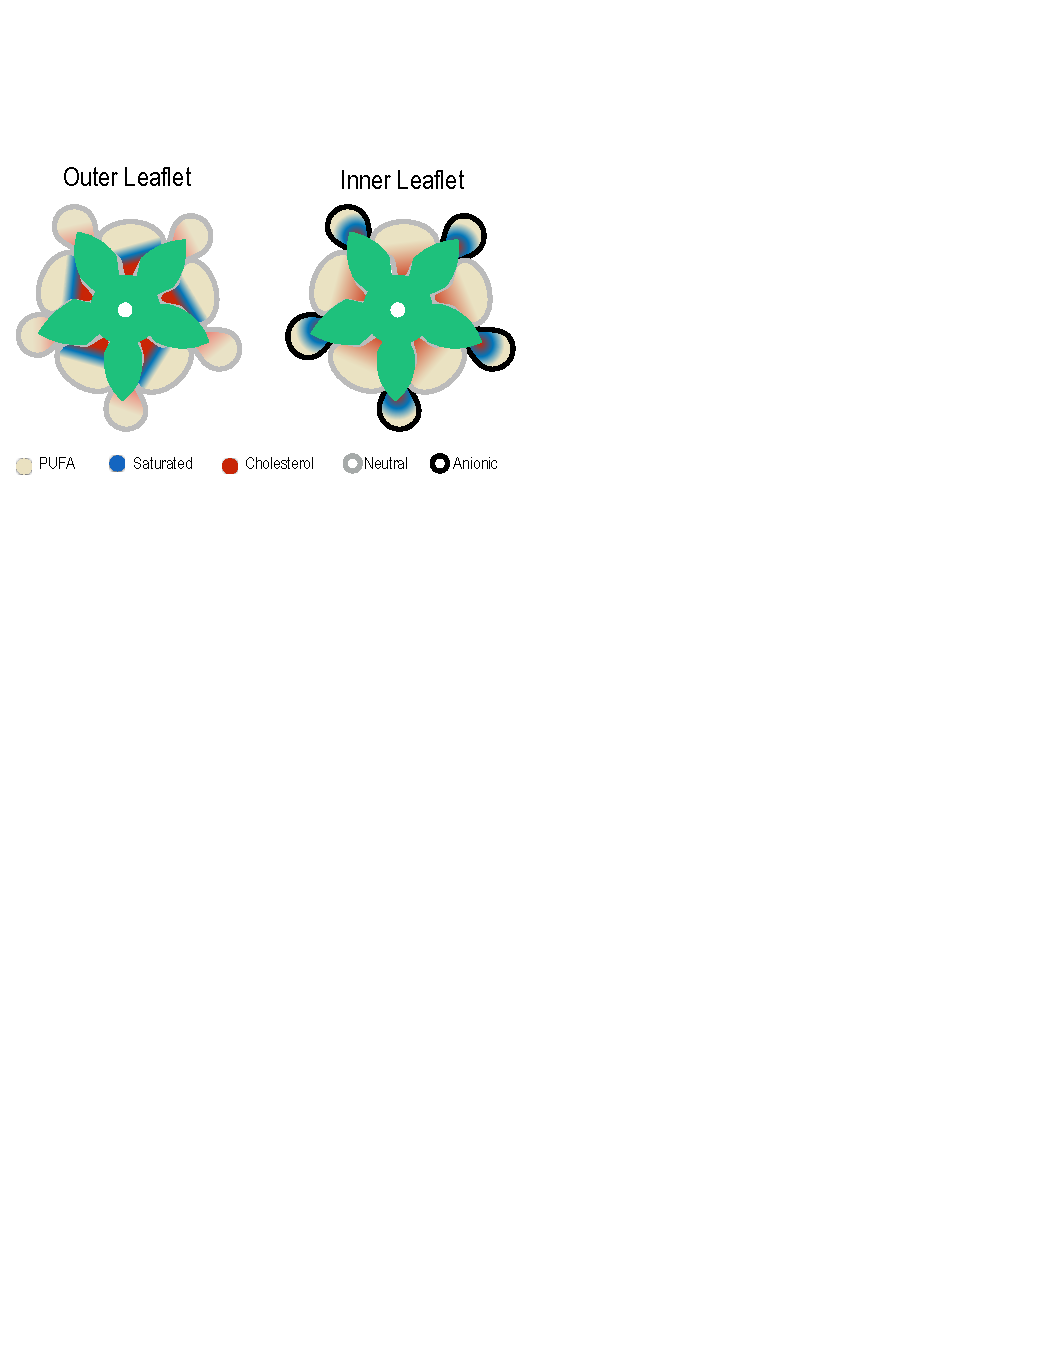
\includegraphics[width=\linewidth]{Summary.pdf}
	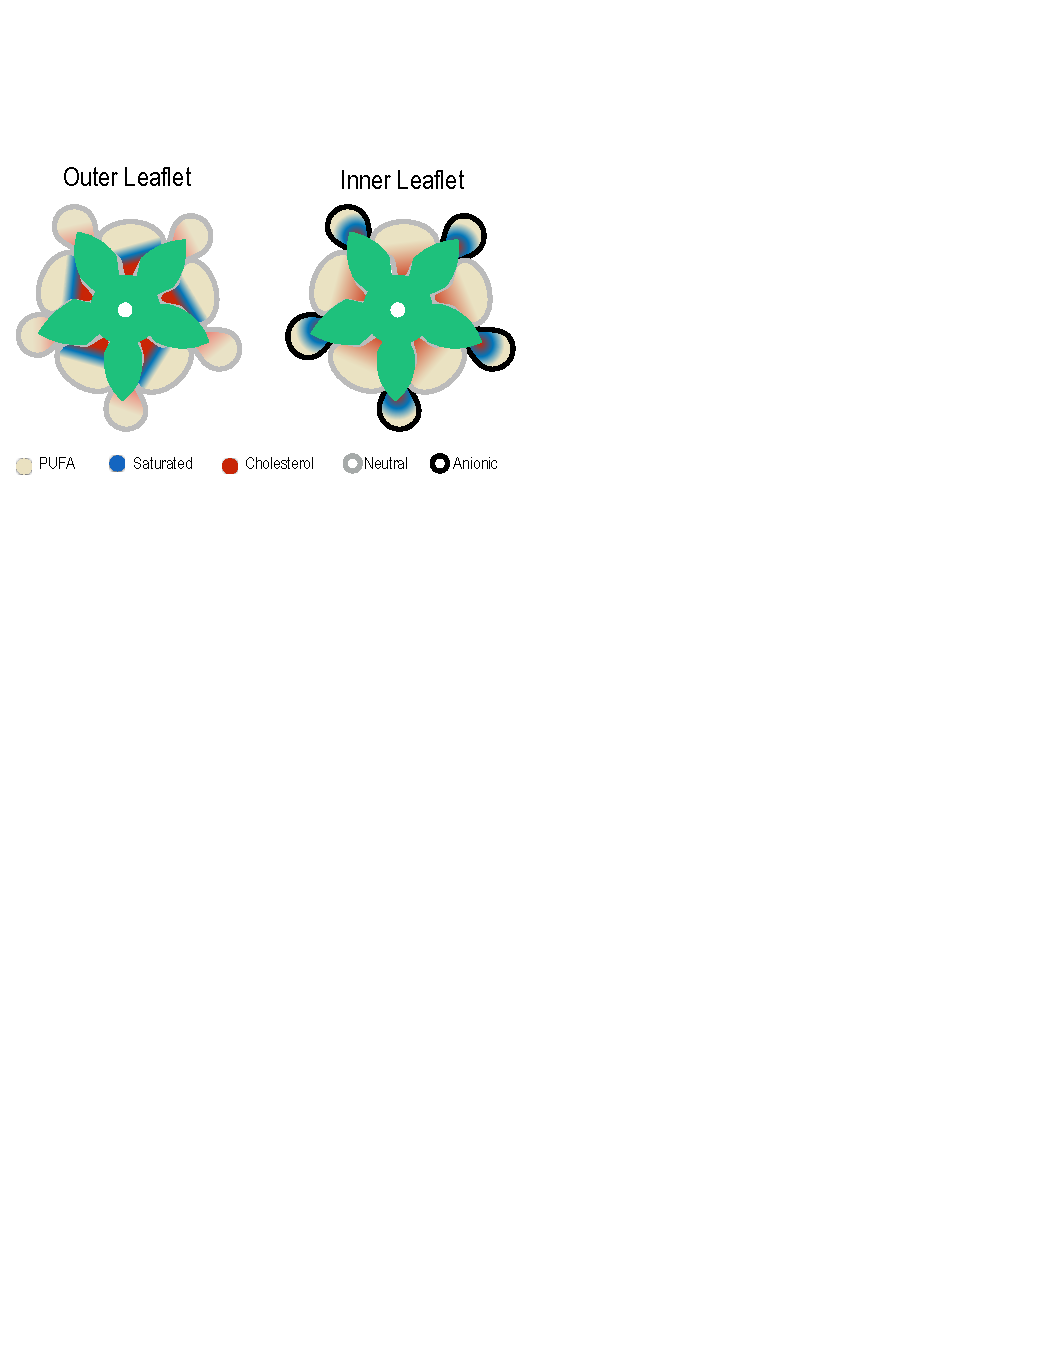
\includegraphics[width=3.5in]{Summary.pdf}
	\caption{{Cartoon of expected boundary lipids for the \nachr~ in a native membrane for both leaflets}. Protein is shown in the center of both leaflets in a cyan floral shape. Grey and black outlines depict sites favorable for neutral and anionic lipids respectively. Fill color represents the lipids most likely to occupy each site (red: cholesterol, blue: saturated, beige: PUFA) and outline represents headgroup charge (gray: neutral, black: anionic).}
	\label{fig:sum}
\end{figure}

Our results are summarized graphically in Figure \ref{fig:sum}. Based on our results from model membranes, we had hypothesized that
%We used a neuronal lipid compositions modified from\cite{Ingolfsson2017b} to analyze \nachr~within a neuronal membrane. We defined lipid-protein occupancy from polar enrichemnt density plots and used Sharp\cite{Sharp2019}, Woods\cite{Woods2019}, and Tong\cite{Tong2019} to hypothesized lipid occupancy for each site. We hypothesized 
 PUFAs would select for the convex M4 sites and that raft-forming lipids like cholesterol and saturated lipids would select for the concave inter-subunit sites. Overall, our results were consistent with this expectation.  Yet although lipids containing PUFAs do prefer the M4 site to the inter-subunit site, their affinity for even the inter-subunit sites are stronger than that of all other phospholipids. This result underscores the reliable partitioning of \nachr{} to PUFA-rich, liquid-disordered domains that we observed in homoacidic, domain forming membranes\cite{Sharp2019}, and suggests PUFAs may have been absent from the inter-subunit site in heteroacidic membranes\cite{Woods2019} because of the constraints of the lipid topology. In the latter simulations, all lipids contained one saturated chain and one PUFA chain, so binding of the PUFA chain to its preferred M4 site requires the saturated chain to find the most favorable location nearby (in the inter-subunit site) and may block binding of other PUFA chains to that site.  These constraints are relaxed in the native neuronal membrane, which has a more diverse lipid composition with multiple different chain pairings; about 6\% of the phospholipids in our simulated membranes contain no saturated chain at all. Nonetheless, our previous results\cite{Woods2019} using simplified binary heteroacidic/cholesterol membranes played a key role in identifying the natural site boundaries.  

As expected, within each leaflet cholesterol has the strongest affinity for the inter-subunit sites, although the affinity of cholesterol for the M4 sites was second only to that of n-3 PUFAs. Combined, these results are consistent with an overwhelming amount of evidence spanning four decades that suggests direct interactions between cholesterol and \nachr s, regardless of the phospholipid composition of the membrane.  One surprise for cholesterol was the role of the leaflet in determining affinity: cholesterol has a stronger affinity for either outer leaflet site compared to either inner leaflet site. This result may reflect competition with anionic saturated lipids in the inner leaflet, which would be consistent with multiple experiments\cite{Baenziger2000,Wenz2005,Hamouda2006,Thompson2020}, suggesting that anionic lipids can partially or fully compensate for a loss of cholesterol.  This result is also consistent with models of cholesterol embedded\cite{Brannigan2008} in the outer TMD (which has numerous gaps in the amino acid density) but not the inner TMD. 
%Of the phospholipids analyzed, n-3 PUFAs have the strongest affinities across all sites, with affinities values of $\sim<0$ kcal/mol for M4 sites and $\sim<$.5 kcal/mol for inter-subunit sites. %We predict the relative high affinity for n-3 PUFAs are a result of their flexibility. The n-3 PUFA, DHA, has a number of unique membrane properties \cite{Stillwell2003a,Gawrisch2003}, and is observed to consistently interact with non-annular sites in and around \plgic s \cite{Sharp2019, Woods2019}. The inherent disorder in PUFAs and the strong affinity they have for M4 sites suggests PUFAs may minimize unfavorable membrane deformation\cite{Brannigan2006,Brannigan2007,Hu2012a,Argudo2016a,BuganzaTepole2017,Dan1993,Fournier2015} around \plgic's conical-star shape provided by M4.
%Similar to n-3 PUFAs cholesterol occupies sites nearly indiscriminately, though for each leaflet cholesterol has the strongest affinity at inter-subunit site. Cholesterol's affinity for the M4, compared to inter-subunit sites, is reduced by about $50\%$ and $80\%$ for the outer and inner leaflets respectively. However, unlike the phospholipids, cholesterol's affinity for each site is consistently $<0$ kcal/mol. %Brannigan et al 2008 \cite{Brannigan2008} hypothesized 15 non-annular cholesterol binding sites for \nachr. Sharp et al 2019 \cite{Sharp2019} observed cholesterol embedded in $\beta$ subunits of \nachr. It could be cholesterol's favorability for M4 is a result of its relative small size making it ideal for packing between alpha-helices.

%For most sites monounsaturated lipids have the weakest affinities ($>.5$ kcal/mol). We hypothesize this is due to packing limitation from monounsaturated lipids single acyl-chain kink. Cholesterol and PUFAs are small or highly flexible and readily fit at various sites in \plgic's topology. Saturated lipids, which lack any kinks and are more rigid than unsaturated lipids, may pack around inter-subunit site's ''flat'' topology. We argue the single acyl-chain kink found in monounsaturated lipids may prevent packing of itself around inter-subunit sites, and is not flexibility to compete with PUFA's occupying M4 sites. 

%Neutral lipids that occupy M4 have a unique trend in affinity. The affinity strength increase as a relation to acyl-chain flexibility, initially state in section \textit{Effect of Acyl-Chain on Neutral Lipid Affinities}. Neutral lipids at inter-subunit sites and all anionic lipids share a non-monotonic affinity trend where it is more akin to a concave function, see Figure \ref{fig:sum}. 

Based on our results using ELIC\cite{Tong2019}, we had expected that anionic lipids would select for sites on the inner leaflet lined with basic residues.  In the homomeric ELIC, these residues are symmetrically-arranged, while in the heteromeric \nachr{} they vary by subunit (\liam{Figure SI 2A}), with the M4 site containing the most such residues on most subunits. The present results support that expectation: %Yet unlike ELIC due to cationic amino acid distribution, see Figure \ref{fig:aaa}a. \nachr~ has cationic amino acids at both inter-subunit and M4 sites.
%Neutral lipids have a stronger affinity for the outer leaflet compared to anionic lipids. Neutral lipids found at the inner inter-subunit sites have slightly weaker affinities compared to the same lipids in the outer inter-subunit site. 
anionic lipids have a stronger affinity for M4 than inter-subunit sites.  %Inner anionic saturated, n-6 and n-3 PUFAs have significantly greater affinities than outer anionic lipids of the same saturation types. Monounsaturated lipids affinity values do not change much between leaflets ($\sim 0.5$ kcal/mol). We associate anionic lipids have stronger affinity for M4 in \nachr~compared to ELIC due to cationic amino acid distribution, see Figure \ref{fig:aaa}a. \nachr~ has cationic amino acids at both inter-subunit and M4 sites.

For both outer and inner leaflets, lipids with a PE head group have stronger affinities than those with a PC head group. \grace{This result is consistent with our previous coarse-grained simulations\cite{Sharp2019, Tong2019} as well as experimental data\cite{Tong2019}. The most straightforward explanation might involve the smaller size of the PE headgroup, which could facilitate acyl chains getting tangled in the protein TMD. These subtle differences in steric hindrance between PE and PC are not captured in MARTINI 2.2, however.  The effective size of the PE headgroup in MARTINI is still smaller than that of PC because it has a stronger attraction to several species of ``nonpolar'' and charged beads in the MARTINI forcefield, which mimics PE's ability to donate hydrogen bonds. The increased affinity of PE for the protein may have a similar origin, because the protein has many hydrogen bond acceptors. Further investigation of the role of hydrogen bonding between the PE headgroup and the protein will require an atomistic forcefield.}  

Among anionic lipids in the inner leaflet, regardless of the site, PS and PI have an affinity greater than or equal to PC, and much greater than the other anionic lipid headgroups (PIP1,PIP2,PIP3, and PA).   The lipid headgroups PS and PI both have a charge of -1, while PA in the MARTINI forcefield\cite{DeJong2012} carries a charge of -2, and PIP1, PIP2, and PIP3 have charges of -3,-5, and -7. These results suggest that the inner leaflet sites select for monoanionic headgroups, while multianionic headgroups are highly unfavorable.  Due to the limitations of the coarse-grained model, future atomistic calculations are required to validate and understand the apparent preference of the M4 site for PI over PS.  %These differences cannot be attributed to size alone: the bulkier PI (four martini beads) and the small PS (two martini beads) have comparable affinities which are both much greater than both the bulky PIPS and the smallest headgroup, PA. 

\grace{All results presented here relied on a single coarse-grained model.  Although a specific group of predictions that we previously made using MARTINI were validated with experiments\cite{Tong2019}, all coarse-grained force-fields have limitations. Pitfalls of the MARTINI 2.2 model have been discussed extensively. \cite{Alessandri2019} Our particular study investigates the ligand-like properties of lipids, and ligand binding of any kind suffers from a coarse-grained treatment due to significant smoothing of the molecular surfaces. Furthermore, many of the effects we investigate here concern lipid chain flexibility, and the chain loses degrees of freedom through the 4-to-1 mapping of the MARTINI model.  Consequently, we expect that coarse-graining should generally reduce selectivity among neutral lipids, and that the equivalent calculations using an atomistic model could yield a much wider range of binding affinities.  Here, we have identified several lipid-site pairs for testing by methods for binding affinities using atomistic lipids, such as alchemical free energy perturbation.\cite{Salari2019} }

The present results highlight the utility of model membranes for developing hypotheses of specific lipid-protein interactions, and the need to test those hypothesis within more complex native membranes. They could also be tested and aid in interpretation of experiments carried out in more complex membranes. For instance, we would expect that mutations of the basic residues facing the inner leaflet would reduce binding of saturated phospholipids with anionic headgroups, which would be replaced with bound cholesterol. We would also predict that if PUFAs cause gain of function via binding to the \liam{inter-subunit} site, this gain would be enhanced by replacing some heteroacidic lipids with homoacidic lipids while keeping the total fraction of PUFA chains constant. In general the present results provide valuable insight into how to predict lipid competition, which is one of the primarily challenges of interpreting experiments in complex membranes.  
%.  PA has the weakest affinity of the anionic lipids, though it has the smallest head group (only a phosphate), and PIPS which are much bulkier than all the other head groups are comparable to PA. PI, PS  share the same charge: -1.0 C. 


%Why one head group interacts more favorably is still unknown. It may be a product of head group to acyl-chain combination, evolution, or the coarse grained model. The PE head group bead types are Qd and Qa, which are attracted to most of the other bead types. PS has P5 and a QA, where P5 is attractive to about half the bead types and repulsive to the other half. PI has coarse-grained ring of P5 and P1s, and Qa, all of which tend to be attractive to other beads.  

%It is unclear why neutral and anionic head group affinities are uncorrelated, though it may be a product of head group to acyl-chain combination, evolution, or the coarse grained model. \notsure{The PE head group bead types are Qd and Qa, which are attracted to most of the other bead types. PS has P5 which is attractive to about half the bead types and repulsive to the other half. PI has coarse-grained ring of P5 and P1s, and Qa, all of which tend to be attractive to other beads. }

%\nachr~lipid occupancy appears to be driven in two steps. First a ''coarse-sorting'' by head groups, and second ''fine-sorting'' by acyl-chains. In the outer leaflet anionic lipids are clearly unfavorable, coarse-sorting. A neutral lipid will occupy \nachr's boundary region and then there is ''fine-sorting'' by acyl-chain saturation. Inner Inter subunit sites have competition between lipid head group charge, but have specific acyl-chain affinity. The inner M4 site has the strongest affinity for anionic lipids regardless of saturation type, which diverges from the proposed occupancy driver. 
%
%Inner anionic lipid occupancy could be driven by another mechanism: anionic lipids occupy M4 due to the number of positively charged amino acids until the site is saturated with anionic lipids, similar to Tong et al\cite{Tong2019}. The remainder anionic lipids do not defusing back to the bulk membrane, they weakly interact with the inner inter-subunit site as a local anionic lipid pool for M4. 

% Raft forming lipids have higher affinities for inter-subunit sites over M4, but cholesterol has unexpectedly strong affinity for all sites. Unsaturated lipids have a highest affinity for M4, however, n-3 PUFAs show strong affinity for inter-subunit sites as well  with a difference of about 1 kcal/mol. These results suggest when neutral lipids are available for \nachr's boundary membrane, degree of saturation and molecule size play vital roles. Saturated and monounsaturated lipids, which tend to maintain a higher degree of order when compared to  PUFAs, show poor affinity in-comparison to more flexible lipids. While, saturated and monounsaturated lipids show relative high and low affinity sites within their saturation species, highly flexible PUFAs and small cholesterol occupy \nachr's density gaps more readily.

\section*{Supplementary Material}

See the supplementary material for neuronal membrane composition, lipid probability distributions, additional binding affinity tables, and details of the site boundaries. 

\section*{Acknowledgments}
GB and LS were supported by the Busch Biomedical Foundation. This project was supported by generous allocation through the Rutgers University Office of Advanced Research Computing (OARC), which is supported by Rutgers University and the state of New Jersey. We are grateful to Dr. J{\'{e}}r{\^{o}}me H{\'{e}}nin for helpful input and suggestions.

\section*{Data Availability Statement}
The data that support the findings of this study are available from the corresponding author upon reasonable request. Scripts for polar density analysis and plotting scripts can be found on github: https://github.com/BranniganLab/densitymap. 
%Using $\Delta G$ free energy to calculate the occupancy affinities, we find n-3 PUFAs and cholesterol \textit{nearly} indiscriminately occupy any region of the protein, cholesterol favors inter-subunit sites and n-3 PUFAs favor M4 sites. Anionic lipids are unfavorable in the outer leaflet. Anionic lipids and neutral lipids occupy at comparable affinities in the inner inter-subunit sites, see Figure \ref{fig:sum}.

%These results show a significant divergence from our proposed hypothesis and are depicted in figure \ref{fig:sum}. In the outer leaflet neutral have a strong affinity to occupy sites. Unsaturated lipids and cholesterol occupy the M4 site, while n-3 PUFAs, cholesterol, and saturated lipids occupy inter-subunit sites. Neutral and anionic lipids occupy inner inter-subunit sites with similar lipid composition compared to the outer leaflet. Inner M4 sites have a strong affinity for anionic lipids regardless of acyl chain.

%% The Appendices part is started with the command \appendix;
%% appendix sections are then done as normal sections
%% \appendix

%% \section{}
%% \label{}

%% References
%%
%% Following citation commands can be used in the body text:
%% Usage of \cite is as follows:
%%   \cite{key}          ==>>  [#]
%%   \cite[chap. 2]{key} ==>>  [#, chap. 2]
%%   \citet{key}         ==>>  Author [#]

%% References with bibTeX database:

\bibliographystyle{model1-num-names}
\begin{thebibliography}{107}
\expandafter\ifx\csname natexlab\endcsname\relax\def\natexlab#1{#1}\fi
\providecommand{\bibinfo}[2]{#2}
\ifx\xfnm\relax \def\xfnm[#1]{\unskip,\space#1}\fi
%Type = Article
\bibitem[{H{\'{e}}nault et~al.(2015)H{\'{e}}nault, Sun, Therien, DaCosta,
  Carswell, Labriola, Juranka, and Baenziger}]{Henault2015}
\bibinfo{author}{C.~M. H{\'{e}}nault}, \bibinfo{author}{J.~Sun},
  \bibinfo{author}{J.~P.~D. Therien}, \bibinfo{author}{C.~J.~B. DaCosta},
  \bibinfo{author}{C.~L. Carswell}, \bibinfo{author}{J.~M. Labriola},
  \bibinfo{author}{P.~F. Juranka}, \bibinfo{author}{J.~E. Baenziger},
\newblock \bibinfo{title}{{The role of the M4 lipid-sensor in the folding,
  trafficking, and allosteric modulation of nicotinic acetylcholine
  receptors}},
\newblock \bibinfo{journal}{Neuropharmacology} \bibinfo{volume}{96}
  (\bibinfo{year}{2015}) \bibinfo{pages}{157--168}.
%Type = Article
\bibitem[{Mukhtasimova et~al.(2016)Mukhtasimova, DaCosta, and
  Sine}]{Mukhtasimova2016}
\bibinfo{author}{N.~Mukhtasimova}, \bibinfo{author}{C.~J.~B. DaCosta},
  \bibinfo{author}{S.~M. Sine},
\newblock \bibinfo{title}{{Improved resolution of single channel dwell times
  reveals mechanisms of binding, priming, and gating in muscle AChR}},
\newblock \bibinfo{journal}{The Journal of General Physiology}
  \bibinfo{volume}{148} (\bibinfo{year}{2016}) \bibinfo{pages}{43--63}.
%Type = Article
\bibitem[{Kalamida et~al.(2007)Kalamida, Poulas, Avramopoulou, Fostieri,
  Lagoumintzis, Lazaridis, Sideri, Zouridakis, and Tzartos}]{Kalamida2007}
\bibinfo{author}{D.~Kalamida}, \bibinfo{author}{K.~Poulas},
  \bibinfo{author}{V.~Avramopoulou}, \bibinfo{author}{E.~Fostieri},
  \bibinfo{author}{G.~Lagoumintzis}, \bibinfo{author}{K.~Lazaridis},
  \bibinfo{author}{A.~Sideri}, \bibinfo{author}{M.~Zouridakis},
  \bibinfo{author}{S.~J. Tzartos},
\newblock \bibinfo{title}{{Muscle and neuronal nicotinic acetylcholine
  receptors: Structure, function and pathogenicity}},
\newblock \bibinfo{journal}{FEBS Journal} \bibinfo{volume}{274}
  (\bibinfo{year}{2007}) \bibinfo{pages}{3799--3845}.
%Type = Article
\bibitem[{Taly et~al.(2009)Taly, Corringer, Guedin, Lestage, and
  Changeux}]{Taly2009}
\bibinfo{author}{A.~Taly}, \bibinfo{author}{P.-J. Corringer},
  \bibinfo{author}{D.~Guedin}, \bibinfo{author}{P.~Lestage},
  \bibinfo{author}{J.-P. Changeux},
\newblock \bibinfo{title}{{Nicotinic receptors: allosteric transitions and
  therapeutic targets in the nervous system}},
\newblock \bibinfo{journal}{Nature Reviews Drug Discovery} \bibinfo{volume}{8}
  (\bibinfo{year}{2009}) \bibinfo{pages}{733--750}.
%Type = Article
\bibitem[{Patel et~al.(2017)Patel, McIntire, Ryan, Dunah, and
  Loring}]{Patel2017}
\bibinfo{author}{H.~Patel}, \bibinfo{author}{J.~McIntire},
  \bibinfo{author}{S.~Ryan}, \bibinfo{author}{A.~Dunah},
  \bibinfo{author}{R.~Loring},
\newblock \bibinfo{title}{Anti-inflammatory effects of astroglial {$\alpha$}7
  nicotinic acetylcholine receptors are mediated by inhibition of the
  {NF-{$\kappa$}B} pathway and activation of the {Nrf2} pathway.},
\newblock \bibinfo{journal}{Journal of neuroinflammation} \bibinfo{volume}{14}
  (\bibinfo{year}{2017}) \bibinfo{pages}{192}.
%Type = Article
\bibitem[{Yocum et~al.(2017)Yocum, Turner, Danielsson, Barajas, Zhang, Xu,
  Harrison, Homanics, Farber, and Emala}]{Yocum2017}
\bibinfo{author}{G.~T. Yocum}, \bibinfo{author}{D.~L. Turner},
  \bibinfo{author}{J.~Danielsson}, \bibinfo{author}{M.~B. Barajas},
  \bibinfo{author}{Y.~Zhang}, \bibinfo{author}{D.~Xu}, \bibinfo{author}{N.~L.
  Harrison}, \bibinfo{author}{G.~E. Homanics}, \bibinfo{author}{D.~L. Farber},
  \bibinfo{author}{C.~W. Emala},
\newblock \bibinfo{title}{{GABA A receptor alpha4-subunit knockout enhances
  lung inflammation and airway reactivity in a murine asthma model}},
\newblock \bibinfo{journal}{American Journal of Physiology - Lung Cellular and
  Molecular Physiology} \bibinfo{volume}{313} (\bibinfo{year}{2017})
  \bibinfo{pages}{L406----L415}.
%Type = Misc
\bibitem[{Egea et~al.(2015)Egea, Buendia, Parada, Navarro, Le{\'{o}}n, and
  Lopez}]{Egea2015}
\bibinfo{author}{J.~Egea}, \bibinfo{author}{I.~Buendia},
  \bibinfo{author}{E.~Parada}, \bibinfo{author}{E.~Navarro},
  \bibinfo{author}{R.~Le{\'{o}}n}, \bibinfo{author}{M.~G. Lopez},
  \bibinfo{title}{{Anti-inflammatory role of microglial alpha7 nAChRs and its
  role in neuroprotection}}, \bibinfo{year}{2015}.
%Type = Article
\bibitem[{Cornelison et~al.(2016)Cornelison, Pflanz, Tipps, and
  Mihic}]{Cornelison2016}
\bibinfo{author}{G.~L. Cornelison}, \bibinfo{author}{N.~C. Pflanz},
  \bibinfo{author}{M.~E. Tipps}, \bibinfo{author}{S.~J. Mihic},
\newblock \bibinfo{title}{{Identification and characterization of heptapeptide
  modulators of the glycine receptor}},
\newblock \bibinfo{journal}{European Journal of Pharmacology}
  \bibinfo{volume}{780} (\bibinfo{year}{2016}) \bibinfo{pages}{252--259}.
%Type = Article
\bibitem[{Xiong et~al.(2012)Xiong, Cui, Cheng, Yang, Chen, Willenbring, Guan,
  Pan, Ren, Xu, and Zhang}]{Xiong2012}
\bibinfo{author}{W.~Xiong}, \bibinfo{author}{T.~Cui},
  \bibinfo{author}{K.~Cheng}, \bibinfo{author}{F.~Yang}, \bibinfo{author}{S.-R.
  Chen}, \bibinfo{author}{D.~Willenbring}, \bibinfo{author}{Y.~Guan},
  \bibinfo{author}{H.-L. Pan}, \bibinfo{author}{K.~Ren},
  \bibinfo{author}{Y.~Xu}, \bibinfo{author}{L.~Zhang},
\newblock \bibinfo{title}{{Cannabinoids suppress inflammatory and neuropathic
  pain by targeting alpha3 glycine receptors}},
\newblock \bibinfo{journal}{The Journal of Experimental Medicine}
  \bibinfo{volume}{209} (\bibinfo{year}{2012}) \bibinfo{pages}{1121--1134}.
%Type = Article
\bibitem[{Walstab et~al.(2010)Walstab, Rappold, and Niesler}]{Walstab2010}
\bibinfo{author}{J.~Walstab}, \bibinfo{author}{G.~Rappold},
  \bibinfo{author}{B.~Niesler},
\newblock \bibinfo{title}{{5-HT(3) receptors: role in disease and target of
  drugs}},
\newblock \bibinfo{journal}{Pharmacology {\&} Therapeutics}
  \bibinfo{volume}{128} (\bibinfo{year}{2010}) \bibinfo{pages}{146--169}.
%Type = Article
\bibitem[{Picciotto(2008)}]{Picciotto_Neuroprotection_2008}
\bibinfo{author}{R.~Picciotto, Marina},
\newblock \bibinfo{title}{{Neuroprotection via nAChRs: the role of nAChRs in
  neurodegenerative disorders such as Alzheimer's and Parkinson's disease}},
\newblock \bibinfo{journal}{Frontiers in Bioscience} \bibinfo{volume}{13}
  (\bibinfo{year}{2008}) \bibinfo{pages}{492}.
%Type = Article
\bibitem[{Martin-Ruiz et~al.(1999)Martin-Ruiz, Court, Molnar, Lee, Gotti,
  Mamalaki, Tsouloufis, Tzartos, Ballard, Perry, and Perry}]{MartinRuiz_4_1999}
\bibinfo{author}{C.~M. Martin-Ruiz}, \bibinfo{author}{J.~A. Court},
  \bibinfo{author}{E.~Molnar}, \bibinfo{author}{M.~Lee},
  \bibinfo{author}{C.~Gotti}, \bibinfo{author}{A.~Mamalaki},
  \bibinfo{author}{T.~Tsouloufis}, \bibinfo{author}{S.~Tzartos},
  \bibinfo{author}{C.~Ballard}, \bibinfo{author}{R.~H. Perry},
  \bibinfo{author}{E.~K. Perry},
\newblock \bibinfo{title}{{Alpha4 but not alpha3 and alpha7 nicotinic
  acetylcholine receptor subunits are lost from the temporal cortex in
  Alzheimer's disease}},
\newblock \bibinfo{journal}{Journal of Neurochemistry} \bibinfo{volume}{73}
  (\bibinfo{year}{1999}) \bibinfo{pages}{1635--1640}.
%Type = Article
\bibitem[{Arnold et~al.(2004)Arnold, Gueye, Guettier-Sigrist, Courdier-Fruh,
  Coupin, Poindron, and Gies}]{Arnold_Reduced_2004}
\bibinfo{author}{A.~S. Arnold}, \bibinfo{author}{M.~Gueye},
  \bibinfo{author}{S.~Guettier-Sigrist}, \bibinfo{author}{I.~Courdier-Fruh},
  \bibinfo{author}{G.~Coupin}, \bibinfo{author}{P.~Poindron},
  \bibinfo{author}{J.~P. Gies},
\newblock \bibinfo{title}{{Reduced expression of nicotinic AChRs in myotubes
  from spinal muscular atrophy I patients}},
\newblock \bibinfo{journal}{Laboratory Investigation} \bibinfo{volume}{84}
  (\bibinfo{year}{2004}) \bibinfo{pages}{1271--1278}.
%Type = Article
\bibitem[{Haydar and Dunlop(2010)}]{Haydar2010}
\bibinfo{author}{S.~N. Haydar}, \bibinfo{author}{J.~Dunlop},
\newblock \bibinfo{title}{Neuronal nicotinic acetylcholine receptors - targets
  for the development of drugs to treat cognitive impairment associated with
  schizophrenia and alzheimer's disease.},
\newblock \bibinfo{journal}{Current topics in medicinal chemistry}
  \bibinfo{volume}{10} (\bibinfo{year}{2010}) \bibinfo{pages}{144--152}.
%Type = Article
\bibitem[{Lennon et~al.(2003)Lennon, Ermilov, Szurszewski, and
  Vernino}]{Lennon_Immunization_2003}
\bibinfo{author}{V.~A. Lennon}, \bibinfo{author}{L.~G. Ermilov},
  \bibinfo{author}{J.~H. Szurszewski}, \bibinfo{author}{S.~Vernino},
\newblock \bibinfo{title}{{Immunization with neuronal nicotinic acetylcholine
  receptor induces neurological autoimmune disease}},
\newblock \bibinfo{journal}{Journal of Clinical Investigation}
  \bibinfo{volume}{111} (\bibinfo{year}{2003}) \bibinfo{pages}{907--913}.
%Type = Article
\bibitem[{Kumari et~al.(2008)Kumari, Borroni, Chaudhry, Chanda, Massol, Mayor,
  and Barrantes}]{Kumari2008}
\bibinfo{author}{S.~Kumari}, \bibinfo{author}{V.~Borroni},
  \bibinfo{author}{A.~Chaudhry}, \bibinfo{author}{B.~Chanda},
  \bibinfo{author}{R.~Massol}, \bibinfo{author}{S.~Mayor},
  \bibinfo{author}{F.~J. Barrantes},
\newblock \bibinfo{title}{{Nicotinic acetylcholine receptor is internalized via
  a Rac-dependent, dynamin-independent endocytic pathway}},
\newblock \bibinfo{journal}{Journal of Cell Biology} \bibinfo{volume}{181}
  (\bibinfo{year}{2008}) \bibinfo{pages}{1179--1193}.
%Type = Article
\bibitem[{Baenziger et~al.(2017)Baenziger, Domville, and
  Therien}]{Baenziger2017}
\bibinfo{author}{J.~E. Baenziger}, \bibinfo{author}{J.~A. Domville},
  \bibinfo{author}{J.~P.~D. Therien},
\newblock \bibinfo{title}{The role of cholesterol in the activation of
  nicotinic acetylcholine receptors.},
\newblock \bibinfo{journal}{Current topics in membranes} \bibinfo{volume}{80}
  (\bibinfo{year}{2017}) \bibinfo{pages}{95--137}.
%Type = Article
\bibitem[{Dalziel et~al.(1980)Dalziel, Rollins, and McNamee}]{Dalziel1980}
\bibinfo{author}{A.~W. Dalziel}, \bibinfo{author}{E.~S. Rollins},
  \bibinfo{author}{M.~G. McNamee},
\newblock \bibinfo{title}{{The effect of cholesterol on agonist-induced flux in
  reconstituted acetylcholine receptor vesicles}},
\newblock \bibinfo{journal}{FEBS Letters} \bibinfo{volume}{122}
  (\bibinfo{year}{1980}) \bibinfo{pages}{193--196}.
%Type = Article
\bibitem[{Ellena et~al.(1983)Ellena, Blazing, and McNamee}]{Ellena1983}
\bibinfo{author}{J.~F. Ellena}, \bibinfo{author}{M.~A. Blazing},
  \bibinfo{author}{M.~G. McNamee},
\newblock \bibinfo{title}{{Lipid-Protein Interactions in Reconstituted
  Membranes Containing Acetylcholine Receptor}},
\newblock \bibinfo{journal}{Biochemistry} \bibinfo{volume}{22}
  (\bibinfo{year}{1983}) \bibinfo{pages}{5523--5535}.
%Type = Article
\bibitem[{Criado et~al.(1983)Criado, Eibl, and Barrantes}]{Criado1983}
\bibinfo{author}{M.~Criado}, \bibinfo{author}{H.~Eibl}, \bibinfo{author}{F.~J.
  Barrantes},
\newblock \bibinfo{title}{{Corrections: Effects of Lipids on Acetylcholine
  Receptor. Essential Need of Cholesterol for Maintenance of Agonist-Induced
  State Transitions in Lipid Vesicles: (Biochemistry (1982) 21(15)
  (3622–3629) (10.1021/bi00258a015))}},
\newblock \bibinfo{journal}{Biochemistry} \bibinfo{volume}{22}
  (\bibinfo{year}{1983}) \bibinfo{pages}{524}.
%Type = Article
\bibitem[{Fong and McNamee(1986)}]{Fong1986}
\bibinfo{author}{T.~M. Fong}, \bibinfo{author}{M.~G. McNamee},
\newblock \bibinfo{title}{{Correlation between acetylcholine receptor function
  and structural properties}},
\newblock \bibinfo{journal}{Biochemistry} \bibinfo{volume}{25}
  (\bibinfo{year}{1986}) \bibinfo{pages}{830--840}.
%Type = Article
\bibitem[{Fong and McNamee(1987)}]{Fong1987}
\bibinfo{author}{T.~M. Fong}, \bibinfo{author}{M.~G. McNamee},
\newblock \bibinfo{title}{{Stabilization of Acetylcholine Receptor Secondary
  Structure by Cholesterol and Negatively Charged Phospholipids in Membranes}},
\newblock \bibinfo{journal}{Biochemistry} \bibinfo{volume}{26}
  (\bibinfo{year}{1987}) \bibinfo{pages}{3871--3880}.
%Type = Article
\bibitem[{Jones and Mcnamee(1988)}]{Jones1988}
\bibinfo{author}{O.~T. Jones}, \bibinfo{author}{M.~G. Mcnamee},
\newblock \bibinfo{title}{{Annular and Nonannular Binding Sites for Cholesterol
  Associated with the Nicotinic Acetylcholine Receptor}},
\newblock \bibinfo{journal}{Biochemistry} \bibinfo{volume}{27}
  (\bibinfo{year}{1988}) \bibinfo{pages}{2364--2374}.
%Type = Article
\bibitem[{Sunshine and McNamee(1994)}]{Sunshine1994}
\bibinfo{author}{C.~Sunshine}, \bibinfo{author}{M.~G. McNamee},
\newblock \bibinfo{title}{{Lipid modulation of nicotinic acetylcholine receptor
  function: the role of membrane lipid composition and fluidity}},
\newblock \bibinfo{journal}{Biochim Biophys Acta} \bibinfo{volume}{1191}
  (\bibinfo{year}{1994}) \bibinfo{pages}{59--64}.
%Type = Article
\bibitem[{DaCosta et~al.(2009)DaCosta, Medaglia, Lavigne, Wang, Carswell, and
  Baenzinger}]{DaCosta2009b}
\bibinfo{author}{C.~J. DaCosta}, \bibinfo{author}{S.~A. Medaglia},
  \bibinfo{author}{N.~Lavigne}, \bibinfo{author}{S.~Wang},
  \bibinfo{author}{C.~L. Carswell}, \bibinfo{author}{J.~E. Baenzinger},
\newblock \bibinfo{title}{{Anionic lipids allosterically modulate multiple
  nicotinic acetylcholine receptor conformational equilibria}},
\newblock \bibinfo{journal}{Journal of Biological Chemistry}
  \bibinfo{volume}{284} (\bibinfo{year}{2009}) \bibinfo{pages}{33841--33849}.
%Type = Article
\bibitem[{Mantipragada et~al.(2003)Mantipragada, Horv{\'{a}}th, Arias,
  Schwarzmann, Sandhoff, Barrantes, and Marsh}]{Mantipragada2003}
\bibinfo{author}{S.~B. Mantipragada}, \bibinfo{author}{L.~I. Horv{\'{a}}th},
  \bibinfo{author}{H.~R. Arias}, \bibinfo{author}{G.~Schwarzmann},
  \bibinfo{author}{K.~Sandhoff}, \bibinfo{author}{F.~J. Barrantes},
  \bibinfo{author}{D.~Marsh},
\newblock \bibinfo{title}{{Lipid-protein interactions and effect of local
  anesthetics in acetylcholine receptor-rich membranes from Torpedo marmorata
  electric organ}},
\newblock \bibinfo{journal}{Biochemistry} \bibinfo{volume}{42}
  (\bibinfo{year}{2003}) \bibinfo{pages}{9167--9175}.
%Type = Article
\bibitem[{Barrantes(2010)}]{Barrantes2010a}
\bibinfo{author}{F.~J. Barrantes},
\newblock \bibinfo{title}{Cholesterol effects on nicotinic acetylcholine
  receptor: cellular aspects.},
\newblock \bibinfo{journal}{Sub-cellular biochemistry} \bibinfo{volume}{51}
  (\bibinfo{year}{2010}) \bibinfo{pages}{467--487}.
%Type = Article
\bibitem[{Baier et~al.(2011)Baier, Fantini, and Barrantes}]{Baier2011a}
\bibinfo{author}{C.~J. Baier}, \bibinfo{author}{J.~Fantini},
  \bibinfo{author}{F.~J. Barrantes},
\newblock \bibinfo{title}{{Disclosure of cholesterol recognition motifs in
  transmembrane domains of the human nicotinic acetylcholine receptor}},
\newblock \bibinfo{journal}{Scientific Reports} \bibinfo{volume}{1}
  (\bibinfo{year}{2011}) \bibinfo{pages}{69}.
%Type = Article
\bibitem[{Zhou et~al.(2003)Zhou, Nelson, Kuryatov, Choi, Cooper, and
  Lindstrom}]{Zhou2003}
\bibinfo{author}{Y.~Zhou}, \bibinfo{author}{M.~E. Nelson},
  \bibinfo{author}{A.~Kuryatov}, \bibinfo{author}{C.~Choi},
  \bibinfo{author}{J.~Cooper}, \bibinfo{author}{J.~Lindstrom},
\newblock \bibinfo{title}{{Human alpha4beta2 acetylcholine receptors formed
  from linked subunits.}},
\newblock \bibinfo{journal}{The Journal of neuroscience : the official journal
  of the Society for Neuroscience} \bibinfo{volume}{23} (\bibinfo{year}{2003})
  \bibinfo{pages}{9004--9015}.
%Type = Article
\bibitem[{Gamba et~al.(2005)Gamba, Hill, Southern, Maciver, Potter, Apodaca,
  Smith, Zeidel, and Warren}]{Gamba2005}
\bibinfo{author}{G.~Gamba}, \bibinfo{author}{W.~G. Hill},
  \bibinfo{author}{N.~M. Southern}, \bibinfo{author}{B.~Maciver},
  \bibinfo{author}{E.~Potter}, \bibinfo{author}{G.~Apodaca},
  \bibinfo{author}{C.~P. Smith}, \bibinfo{author}{M.~L. Zeidel},
  \bibinfo{author}{G.~Warren},
\newblock \bibinfo{title}{{Isolation and characterization of the Xenopus oocyte
  plasma membrane : a new method for studying activity of water and solute
  transporters}},
\newblock \bibinfo{journal}{American Journal of Physiology-Renal Physiology}
  \bibinfo{volume}{15261} (\bibinfo{year}{2005}) \bibinfo{pages}{217--224}.
%Type = Article
\bibitem[{Chen et~al.(2015)Chen, Kinde, Arjunan, Wells, Cohen, Xu, and
  Tang}]{Chen2015}
\bibinfo{author}{Q.~Chen}, \bibinfo{author}{M.~N. Kinde},
  \bibinfo{author}{P.~Arjunan}, \bibinfo{author}{M.~M. Wells},
  \bibinfo{author}{A.~E. Cohen}, \bibinfo{author}{Y.~Xu},
  \bibinfo{author}{P.~Tang},
\newblock \bibinfo{title}{{Direct Pore Binding as a Mechanism for Isoflurane
  Inhibition of the Pentameric Ligand-gated Ion Channel ELIC}},
\newblock \bibinfo{journal}{Scientific Reports} \bibinfo{volume}{5}
  (\bibinfo{year}{2015}) \bibinfo{pages}{13833}.
%Type = Article
\bibitem[{Kouvatsos et~al.(2016)Kouvatsos, Giastas, Chroni-Tzartou,
  Poulopoulou, and Tzartos}]{Kouvatsos2016}
\bibinfo{author}{N.~Kouvatsos}, \bibinfo{author}{P.~Giastas},
  \bibinfo{author}{D.~Chroni-Tzartou}, \bibinfo{author}{C.~Poulopoulou},
  \bibinfo{author}{S.~J. Tzartos},
\newblock \bibinfo{title}{{Crystal structure of a human neuronal nAChR
  extracellular domain in pentameric assembly: Ligand-bound alpha2
  homopentamer}},
\newblock \bibinfo{journal}{Proceedings of the National Academy of Sciences}
  \bibinfo{volume}{113} (\bibinfo{year}{2016}) \bibinfo{pages}{9635--9640}.
%Type = Article
\bibitem[{Nys et~al.(2016)Nys, Wijckmans, Farinha, Yoluk, Andersson, Brams,
  Spurny, Peigneur, Tytgat, Lindahl, and Ulens}]{Nys2016}
\bibinfo{author}{M.~Nys}, \bibinfo{author}{E.~Wijckmans},
  \bibinfo{author}{A.~Farinha}, \bibinfo{author}{{\"{O}}.~Yoluk},
  \bibinfo{author}{M.~Andersson}, \bibinfo{author}{M.~Brams},
  \bibinfo{author}{R.~Spurny}, \bibinfo{author}{S.~Peigneur},
  \bibinfo{author}{J.~Tytgat}, \bibinfo{author}{E.~Lindahl},
  \bibinfo{author}{C.~Ulens},
\newblock \bibinfo{title}{{Allosteric binding site in a Cys-loop receptor
  ligand-binding domain unveiled in the crystal structure of ELIC in complex
  with chlorpromazine}},
\newblock \bibinfo{journal}{Proceedings of the National Academy of Sciences}
  \bibinfo{volume}{113} (\bibinfo{year}{2016}) \bibinfo{pages}{E6696----E6703}.
%Type = Article
\bibitem[{Polovinkin et~al.(2018)Polovinkin, {Gh{\'{e}}rici Hassaine}, Perot,
  Neumann, Jensen, Lefebvre, Corringer, Neyton, Chipot, Dehez, Schoehn, and
  Nury}]{Polovinkin2018}
\bibinfo{author}{L.~Polovinkin}, \bibinfo{author}{G.~{Gh{\'{e}}rici Hassaine}},
  \bibinfo{author}{J.~Perot}, \bibinfo{author}{E.~Neumann},
  \bibinfo{author}{A.~A. Jensen}, \bibinfo{author}{S.~N. Lefebvre},
  \bibinfo{author}{P.-J. Corringer}, \bibinfo{author}{J.~Neyton},
  \bibinfo{author}{C.~Chipot}, \bibinfo{author}{F.~Dehez},
  \bibinfo{author}{G.~Schoehn}, \bibinfo{author}{H.~Nury},
\newblock \bibinfo{title}{{Conformational transitions of the serotonin 5-HT 3
  receptor}},
\newblock \bibinfo{journal}{Nature}  (\bibinfo{year}{2018}).
%Type = Article
\bibitem[{Moffett et~al.(2019)Moffett, Klein, Brannigan, and
  Martin}]{Moffett2019}
\bibinfo{author}{S.~X. Moffett}, \bibinfo{author}{E.~A. Klein},
  \bibinfo{author}{G.~Brannigan}, \bibinfo{author}{J.~V. Martin},
\newblock \bibinfo{title}{{L-3,3$^\prime$,5-triiodothyronine and pregnenolone
  sulfate inhibit Torpedo nicotinic acetylcholine receptors}},
\newblock \bibinfo{journal}{PLoS ONE} \bibinfo{volume}{14}
  (\bibinfo{year}{2019}) \bibinfo{pages}{1--18}.
%Type = Article
\bibitem[{Kumar et~al.(2020)Kumar, Wang, Zhang, Zhao, Cymes, Tajkhorshid, and
  Grosman}]{Kumar2020}
\bibinfo{author}{P.~Kumar}, \bibinfo{author}{Y.~Wang},
  \bibinfo{author}{Z.~Zhang}, \bibinfo{author}{Z.~Zhao}, \bibinfo{author}{G.~D.
  Cymes}, \bibinfo{author}{E.~Tajkhorshid}, \bibinfo{author}{C.~Grosman},
\newblock \bibinfo{title}{{Cryo-EM structures of a lipid-sensitive pentameric
  ligand-gated ion channel embedded in a phosphatidylcholine-only bilayer}},
\newblock \bibinfo{journal}{Proceedings of the National Academy of Sciences of
  the United States of America} \bibinfo{volume}{117} (\bibinfo{year}{2020})
  \bibinfo{pages}{1788--1798}.
%Type = Article
\bibitem[{Conti et~al.(2013)Conti, Limon, Palma, and Miledi}]{Conti2013}
\bibinfo{author}{L.~Conti}, \bibinfo{author}{A.~Limon},
  \bibinfo{author}{E.~Palma}, \bibinfo{author}{R.~Miledi},
\newblock \bibinfo{title}{{Microtransplantation of cellular membranes from
  squid stellate ganglion reveals ionotropic GABA receptors}},
\newblock \bibinfo{journal}{Biological Bulletin} \bibinfo{volume}{224}
  (\bibinfo{year}{2013}) \bibinfo{pages}{47--52}.
%Type = Article
\bibitem[{Cotman et~al.(1969)Cotman, Blank, Moehl, and Snyder}]{Isolated1969}
\bibinfo{author}{C.~Cotman}, \bibinfo{author}{M.~L. Blank},
  \bibinfo{author}{A.~Moehl}, \bibinfo{author}{F.~Snyder},
\newblock \bibinfo{title}{{Lipid Composition of Synaptic Plasma Membranes
  Isolated from Rat Brain by Zonal Centrifugation}},
\newblock \bibinfo{journal}{Biochemistry} \bibinfo{volume}{8}
  (\bibinfo{year}{1969}) \bibinfo{pages}{4606--4612}.
%Type = Article
\bibitem[{Taguchi and Ishikawa(2010)}]{Taguchi2010}
\bibinfo{author}{R.~Taguchi}, \bibinfo{author}{M.~Ishikawa},
\newblock \bibinfo{title}{{Precise and global identification of phospholipid
  molecular species by an Orbitrap mass spectrometer and automated search
  engine Lipid Search}},
\newblock \bibinfo{journal}{Journal of Chromatography A}
  (\bibinfo{year}{2010}).
%Type = Article
\bibitem[{Breckenridge et~al.(1973)Breckenridge, Morgan, Zanetta, and
  Vincendon}]{Breckenridge1973}
\bibinfo{author}{W.~C. Breckenridge}, \bibinfo{author}{I.~G. Morgan},
  \bibinfo{author}{J.~P. Zanetta}, \bibinfo{author}{G.~Vincendon},
\newblock \bibinfo{title}{{Adult rat brain synaptic vesicles II. Lipid
  composition}},
\newblock \bibinfo{journal}{BBA - General Subjects} \bibinfo{volume}{320}
  (\bibinfo{year}{1973}) \bibinfo{pages}{681--686}.
%Type = Article
\bibitem[{Ing{\'{o}}lfsson et~al.(2017)Ing{\'{o}}lfsson, Carpenter, Bhatia,
  Bremer, Marrink, and Lightstone}]{Ingolfsson2017b}
\bibinfo{author}{H.~I. Ing{\'{o}}lfsson}, \bibinfo{author}{T.~S. Carpenter},
  \bibinfo{author}{H.~Bhatia}, \bibinfo{author}{P.~T. Bremer},
  \bibinfo{author}{S.~J. Marrink}, \bibinfo{author}{F.~C. Lightstone},
\newblock \bibinfo{title}{{Computational Lipidomics of the Neuronal Plasma
  Membrane}},
\newblock \bibinfo{journal}{Biophysical Journal} \bibinfo{volume}{113}
  (\bibinfo{year}{2017}) \bibinfo{pages}{2271--2280}.
%Type = Article
\bibitem[{McEvoy et~al.(2000)McEvoy, Coull, Broadbent, Hutchinson, and
  Speake}]{McEvoy2000}
\bibinfo{author}{T.~G. McEvoy}, \bibinfo{author}{G.~D. Coull},
  \bibinfo{author}{P.~J. Broadbent}, \bibinfo{author}{J.~S.~M. Hutchinson},
  \bibinfo{author}{B.~K. Speake},
\newblock \bibinfo{title}{{Fatty acid composition of lipids in immature cattle,
  pig and sheep oocytes with intact zona pellucida}},
\newblock \bibinfo{journal}{J Reprod Fertil} \bibinfo{volume}{118}
  (\bibinfo{year}{2000}) \bibinfo{pages}{163--170}.
%Type = Article
\bibitem[{Kim et~al.(2001)Kim, Kinoshita, Ohnishi, and Fukui}]{Kim2001}
\bibinfo{author}{J.~Y. Kim}, \bibinfo{author}{M.~Kinoshita},
  \bibinfo{author}{M.~Ohnishi}, \bibinfo{author}{Y.~Fukui},
\newblock \bibinfo{title}{{Lipid and fatty acid analysis of fresh and
  frozen-thawed immature and in vitro matured bovine oocytes}},
\newblock \bibinfo{journal}{Reproduction} \bibinfo{volume}{122}
  (\bibinfo{year}{2001}) \bibinfo{pages}{131--138}.
%Type = Article
\bibitem[{van Meer and de~Kroon(2010)}]{VanMeer2010}
\bibinfo{author}{G.~van Meer}, \bibinfo{author}{A.~I. P.~M. de~Kroon},
\newblock \bibinfo{title}{{Lipid map of the mammalian cell}},
\newblock \bibinfo{journal}{Journal of Cell Science} \bibinfo{volume}{124}
  (\bibinfo{year}{2010}) \bibinfo{pages}{5--8}.
%Type = Article
\bibitem[{Lorent et~al.(2020)Lorent, Levental, Ganesan, Rivera-Longsworth,
  Sezgin, Doktorova, Lyman, and Levental}]{Lorent2020}
\bibinfo{author}{J.~H. Lorent}, \bibinfo{author}{K.~R. Levental},
  \bibinfo{author}{L.~Ganesan}, \bibinfo{author}{G.~Rivera-Longsworth},
  \bibinfo{author}{E.~Sezgin}, \bibinfo{author}{M.~Doktorova},
  \bibinfo{author}{E.~Lyman}, \bibinfo{author}{I.~Levental},
\newblock \bibinfo{title}{{Plasma membranes are asymmetric in lipid
  unsaturation, packing and protein shape}},
\newblock \bibinfo{journal}{Nature Chemical Biology} \bibinfo{volume}{16}
  (\bibinfo{year}{2020}) \bibinfo{pages}{644--652}.
%Type = Article
\bibitem[{Ing{\'{o}}lfsson et~al.(2014)Ing{\'{o}}lfsson, Melo, {Van Eerden},
  Arnarez, Lopez, Wassenaar, Periole, {De Vries}, Tieleman, and
  Marrink}]{Ingolfsson2014}
\bibinfo{author}{H.~I. Ing{\'{o}}lfsson}, \bibinfo{author}{M.~N. Melo},
  \bibinfo{author}{F.~J. {Van Eerden}}, \bibinfo{author}{C.~Arnarez},
  \bibinfo{author}{C.~A. Lopez}, \bibinfo{author}{T.~A. Wassenaar},
  \bibinfo{author}{X.~Periole}, \bibinfo{author}{A.~H. {De Vries}},
  \bibinfo{author}{D.~P. Tieleman}, \bibinfo{author}{S.~J. Marrink},
\newblock \bibinfo{title}{{Lipid organization of the plasma membrane}},
\newblock \bibinfo{journal}{Journal of the American Chemical Society}
  \bibinfo{volume}{136} (\bibinfo{year}{2014}) \bibinfo{pages}{14554--14559}.
%Type = Article
\bibitem[{Barrantes(1989)}]{Barrantes1989}
\bibinfo{author}{F.~J. Barrantes},
\newblock \bibinfo{title}{{The lipid environment of the nicotinic acetylcholine
  receptor in native and reconstituted membrane}},
\newblock \bibinfo{journal}{Critical Reviews in Biochemistry and Molecular
  Biology} \bibinfo{volume}{24} (\bibinfo{year}{1989})
  \bibinfo{pages}{437--478}.
%Type = Article
\bibitem[{Quesada et~al.(2016)Quesada, {Gonz{\'{a}}lez -Freire}, Ferrer,
  {Col{\'{o}}n -S{\'{a}}ez}, Fern{\'{a}}ndez-Garc{\'{i}}a, Mercado,
  D{\'{a}}vila, Morales, and Lasalde-Dominicci}]{Quesada2016}
\bibinfo{author}{O.~Quesada}, \bibinfo{author}{C.~{Gonz{\'{a}}lez -Freire}},
  \bibinfo{author}{M.~C. Ferrer}, \bibinfo{author}{J.~O. {Col{\'{o}}n
  -S{\'{a}}ez}}, \bibinfo{author}{E.~Fern{\'{a}}ndez-Garc{\'{i}}a},
  \bibinfo{author}{J.~Mercado}, \bibinfo{author}{A.~D{\'{a}}vila},
  \bibinfo{author}{R.~Morales}, \bibinfo{author}{J.~A. Lasalde-Dominicci},
\newblock \bibinfo{title}{{Uncovering the lipidic basis for the preparation of
  functional nicotinic acetylcholine receptor detergent complexes for
  structural studies}},
\newblock \bibinfo{journal}{Scientific Reports} \bibinfo{volume}{6}
  (\bibinfo{year}{2016}) \bibinfo{pages}{32766}.
%Type = Article
\bibitem[{McNamara et~al.(2006)McNamara, Ostrander, Abplanalp, Richtand,
  Benoit, and Clegg}]{McNamara2006}
\bibinfo{author}{R.~K. McNamara}, \bibinfo{author}{M.~Ostrander},
  \bibinfo{author}{W.~Abplanalp}, \bibinfo{author}{N.~M. Richtand},
  \bibinfo{author}{S.~C. Benoit}, \bibinfo{author}{D.~J. Clegg},
\newblock \bibinfo{title}{{Modulation of phosphoinositide-protein kinase C
  signal transduction by omega-3 fatty acids: Implications for the
  pathophysiology and treatment of recurrent neuropsychiatric illness}},
\newblock \bibinfo{journal}{Prostaglandins Leukotrienes and Essential Fatty
  Acids} \bibinfo{volume}{75} (\bibinfo{year}{2006}) \bibinfo{pages}{237--257}.
%Type = Article
\bibitem[{McNamara et~al.(2008)McNamara, Jandacek, Rider, Tso, Stanford, Hahn,
  and Richtand}]{McNamara2008}
\bibinfo{author}{R.~K. McNamara}, \bibinfo{author}{R.~Jandacek},
  \bibinfo{author}{T.~Rider}, \bibinfo{author}{P.~Tso}, \bibinfo{author}{K.~E.
  Stanford}, \bibinfo{author}{C.~G. Hahn}, \bibinfo{author}{N.~M. Richtand},
\newblock \bibinfo{title}{{Deficits in docosahexaenoic acid and associated
  elevations in the metabolism of arachidonic acid and saturated fatty acids in
  the postmortem orbitofrontal cortex of patients with bipolar disorder}},
\newblock \bibinfo{journal}{Psychiatry Research} \bibinfo{volume}{160}
  (\bibinfo{year}{2008}) \bibinfo{pages}{285--299}.
%Type = Article
\bibitem[{Maekawa et~al.(2017)Maekawa, Watanabe, Iwayama, Kimura, Hamazaki,
  Balan, Ohba, Hisano, Nozaki, Ohnishi, Toyoshima, Shimamoto, Iwamoto, Bundo,
  Osumi, Takahashi, Takashima, and Yoshikawa}]{Maekawa2017}
\bibinfo{author}{M.~Maekawa}, \bibinfo{author}{A.~Watanabe},
  \bibinfo{author}{Y.~Iwayama}, \bibinfo{author}{T.~Kimura},
  \bibinfo{author}{K.~Hamazaki}, \bibinfo{author}{S.~Balan},
  \bibinfo{author}{H.~Ohba}, \bibinfo{author}{Y.~Hisano},
  \bibinfo{author}{Y.~Nozaki}, \bibinfo{author}{T.~Ohnishi},
  \bibinfo{author}{M.~Toyoshima}, \bibinfo{author}{C.~Shimamoto},
  \bibinfo{author}{K.~Iwamoto}, \bibinfo{author}{M.~Bundo},
  \bibinfo{author}{N.~Osumi}, \bibinfo{author}{E.~Takahashi},
  \bibinfo{author}{A.~Takashima}, \bibinfo{author}{T.~Yoshikawa},
\newblock \bibinfo{title}{{Polyunsaturated fatty acid deficiency during
  neurodevelopment in mice models the prodromal state of schizophrenia through
  epigenetic changes in nuclear receptor genes}},
\newblock \bibinfo{journal}{Translational Psychiatry} \bibinfo{volume}{7}
  (\bibinfo{year}{2017}) \bibinfo{pages}{1--11}.
%Type = Misc
\bibitem[{Adibhatla and Hatcher(2007)}]{MuralikrishnaAdibhatla}
\bibinfo{author}{R.~M. Adibhatla}, \bibinfo{author}{J.~F. Hatcher},
  \bibinfo{title}{{Role of lipids in brain injury and diseases}},
  \bibinfo{year}{2007}.
%Type = Misc
\bibitem[{Schneider et~al.(2017)Schneider, Levant, Reichel, Gulbins, Kornhuber,
  and M{\"{u}}ller}]{Schneider2017}
\bibinfo{author}{M.~Schneider}, \bibinfo{author}{B.~Levant},
  \bibinfo{author}{M.~Reichel}, \bibinfo{author}{E.~Gulbins},
  \bibinfo{author}{J.~Kornhuber}, \bibinfo{author}{C.~P. M{\"{u}}ller},
  \bibinfo{title}{{Lipids in psychiatric disorders and preventive medicine}},
  \bibinfo{year}{2017}.
%Type = Article
\bibitem[{Koga et~al.(2019)Koga, Ogura, Yoshida, Hattori, Hori, Aizawa, Ishida,
  and Kunugi}]{Koga2019}
\bibinfo{author}{N.~Koga}, \bibinfo{author}{J.~Ogura},
  \bibinfo{author}{F.~Yoshida}, \bibinfo{author}{K.~Hattori},
  \bibinfo{author}{H.~Hori}, \bibinfo{author}{E.~Aizawa},
  \bibinfo{author}{I.~Ishida}, \bibinfo{author}{H.~Kunugi},
\newblock \bibinfo{title}{{Altered polyunsaturated fatty acid levels in
  relation to proinflammatory cytokines, fatty acid desaturase genotype, and
  diet in bipolar disorder}},
\newblock \bibinfo{journal}{Translational Psychiatry} \bibinfo{volume}{9}
  (\bibinfo{year}{2019}).
%Type = Article
\bibitem[{Hamazaki et~al.(2015)Hamazaki, Maekawa, Toyota, Dean, Hamazaki, and
  Yoshikawa}]{Hamazaki2015}
\bibinfo{author}{K.~Hamazaki}, \bibinfo{author}{M.~Maekawa},
  \bibinfo{author}{T.~Toyota}, \bibinfo{author}{B.~Dean},
  \bibinfo{author}{T.~Hamazaki}, \bibinfo{author}{T.~Yoshikawa},
\newblock \bibinfo{title}{{Fatty acid composition of the postmortem prefrontal
  cortex of patients with schizophrenia, bipolar disorder, and major depressive
  disorder}},
\newblock \bibinfo{journal}{Psychiatry Research} \bibinfo{volume}{227}
  (\bibinfo{year}{2015}) \bibinfo{pages}{353--359}.
%Type = Article
\bibitem[{Peet(2003)}]{Peet2003}
\bibinfo{author}{M.~Peet},
\newblock \bibinfo{title}{{Eicosapentaenoic acid in the treatment of
  schizophrenia and depression: Rationale and preliminary double-blind clinical
  trial results}},
\newblock \bibinfo{journal}{Prostaglandins Leukotrienes and Essential Fatty
  Acids} \bibinfo{volume}{69} (\bibinfo{year}{2003}) \bibinfo{pages}{477--485}.
%Type = Article
\bibitem[{Bushe and Paton(2005)}]{Bushe2005}
\bibinfo{author}{C.~Bushe}, \bibinfo{author}{C.~Paton},
\newblock \bibinfo{title}{{The potential impact of antipsychotics on lipids in
  schizophrenia: Is there enough evidence to confirm a link?}},
\newblock \bibinfo{journal}{Journal of Psychopharmacology} \bibinfo{volume}{19}
  (\bibinfo{year}{2005}) \bibinfo{pages}{76--83}.
%Type = Article
\bibitem[{Berger et~al.(2006)Berger, Smesny, and Amminger}]{Berger2006}
\bibinfo{author}{G.~E. Berger}, \bibinfo{author}{S.~Smesny},
  \bibinfo{author}{G.~P. Amminger},
\newblock \bibinfo{title}{{Bioactive lipids in schizophrenia}},
\newblock \bibinfo{journal}{International Review of Psychiatry}
  \bibinfo{volume}{18} (\bibinfo{year}{2006}) \bibinfo{pages}{85--98}.
%Type = Article
\bibitem[{Conquer et~al.(2000)Conquer, Tierney, Zecevic, Bettger, and
  Fisher}]{Conquer2000}
\bibinfo{author}{J.~A. Conquer}, \bibinfo{author}{M.~C. Tierney},
  \bibinfo{author}{J.~Zecevic}, \bibinfo{author}{W.~J. Bettger},
  \bibinfo{author}{R.~H. Fisher},
\newblock \bibinfo{title}{{Fatty acid analysis of blood plasma of patients with
  alzheimer's disease, other types of dementia, and cognitive impairment}},
\newblock \bibinfo{journal}{Lipids} \bibinfo{volume}{35} (\bibinfo{year}{2000})
  \bibinfo{pages}{1305--1312}.
%Type = Article
\bibitem[{{Di Paolo} and Kim(2011)}]{DiPaolo2011}
\bibinfo{author}{G.~{Di Paolo}}, \bibinfo{author}{T.-W. Kim},
\newblock \bibinfo{title}{{Linking lipids to Alzheimer's disease: cholesterol
  and beyond}},
\newblock \bibinfo{journal}{Nature Reviews Neuroscience} \bibinfo{volume}{12}
  (\bibinfo{year}{2011}) \bibinfo{pages}{284--296}.
%Type = Article
\bibitem[{Bennett et~al.(2013)Bennett, Valenzuela, Xu, Franko, Fai, and
  Figeys}]{Bennett2013}
\bibinfo{author}{S.~A.~L. Bennett}, \bibinfo{author}{N.~Valenzuela},
  \bibinfo{author}{H.~Xu}, \bibinfo{author}{B.~Franko},
  \bibinfo{author}{S.~Fai}, \bibinfo{author}{D.~Figeys},
\newblock \bibinfo{title}{{Using neurolipidomics to identify phospholipid
  mediators of synaptic (dys)function in Alzheimer's Disease}},
\newblock \bibinfo{journal}{Frontiers in Physiology} \bibinfo{volume}{4 JUL}
  (\bibinfo{year}{2013}) \bibinfo{pages}{1--16}.
%Type = Misc
\bibitem[{Yadav and Tiwari(2014)}]{Yadav2014a}
\bibinfo{author}{R.~S. Yadav}, \bibinfo{author}{N.~K. Tiwari},
  \bibinfo{title}{{Lipid Integration in Neurodegeneration: An Overview of
  Alzheimer's Disease}}, \bibinfo{year}{2014}.
%Type = Article
\bibitem[{Escrib{\'{a}}(2017)}]{Escriba2017}
\bibinfo{author}{P.~V. Escrib{\'{a}}},
\newblock \bibinfo{title}{{Membrane-lipid therapy: A historical perspective of
  membrane-targeted therapies — From lipid bilayer structure to the
  pathophysiological regulation of cells}},
\newblock \bibinfo{journal}{Biochimica et Biophysica Acta - Biomembranes}
  \bibinfo{volume}{1859} (\bibinfo{year}{2017}) \bibinfo{pages}{1493--1506}.
%Type = Article
\bibitem[{Addona et~al.(1998)Addona, Sandermann, Kloczewiak, Husain, and
  Miller}]{Addona1998}
\bibinfo{author}{G.~H. Addona}, \bibinfo{author}{H.~Sandermann},
  \bibinfo{author}{M.~A. Kloczewiak}, \bibinfo{author}{S.~S. Husain},
  \bibinfo{author}{K.~W. Miller},
\newblock \bibinfo{title}{{Where does cholesterol act during activation of the
  nicotinic acetylcholine receptor?}},
\newblock \bibinfo{journal}{Biochimica et Biophysica Acta - Biomembranes}
  \bibinfo{volume}{1370} (\bibinfo{year}{1998}) \bibinfo{pages}{299--309}.
%Type = Article
\bibitem[{Laverty et~al.(2017)Laverty, Thomas, Field, Andersen, Gold, Biggin,
  Gielen, and Smart}]{Laverty2017}
\bibinfo{author}{D.~Laverty}, \bibinfo{author}{P.~Thomas},
  \bibinfo{author}{M.~Field}, \bibinfo{author}{O.~J. Andersen},
  \bibinfo{author}{M.~G. Gold}, \bibinfo{author}{P.~C. Biggin},
  \bibinfo{author}{M.~Gielen}, \bibinfo{author}{T.~G. Smart},
\newblock \bibinfo{title}{{Crystal structures of a GABA A -receptor chimera
  reveal new endogenous neurosteroid-binding sites}},
\newblock \bibinfo{journal}{Nature Structural and Molecular Biology}
  \bibinfo{volume}{24} (\bibinfo{year}{2017}) \bibinfo{pages}{977--985}.
%Type = Article
\bibitem[{Budelier et~al.(2019)Budelier, Cheng, Chen, Bracamontes, Sugasawa,
  Krishnan, Mydock-McGrane, Covey, and Evers}]{Budelier2019}
\bibinfo{author}{M.~M. Budelier}, \bibinfo{author}{W.~W.~L. Cheng},
  \bibinfo{author}{Z.~W. Chen}, \bibinfo{author}{J.~R. Bracamontes},
  \bibinfo{author}{Y.~Sugasawa}, \bibinfo{author}{K.~Krishnan},
  \bibinfo{author}{L.~Mydock-McGrane}, \bibinfo{author}{D.~F. Covey},
  \bibinfo{author}{A.~S. Evers},
\newblock \bibinfo{title}{{Common binding sites for cholesterol and
  neurosteroids on a pentameric ligand-gated ion channel}},
\newblock \bibinfo{journal}{Biochimica et Biophysica Acta - Molecular and Cell
  Biology of Lipids} \bibinfo{volume}{1864} (\bibinfo{year}{2019})
  \bibinfo{pages}{128--136}.
%Type = Article
\bibitem[{Basak et~al.(2017)Basak, Schmandt, Gicheru, and
  Chakrapani}]{Basak2017}
\bibinfo{author}{S.~Basak}, \bibinfo{author}{N.~Schmandt},
  \bibinfo{author}{Y.~Gicheru}, \bibinfo{author}{S.~Chakrapani},
\newblock \bibinfo{title}{{Crystal structure and dynamics of a lipid-induced
  potential desensitized-state of a pentameric ligand-gated channel}},
\newblock \bibinfo{journal}{eLife} \bibinfo{volume}{6} (\bibinfo{year}{2017})
  \bibinfo{pages}{e23886}.
%Type = Article
\bibitem[{H{\'{e}}nault et~al.(2019)H{\'{e}}nault, Govaerts, Spurny, Brams,
  Estrada-Mondragon, Lynch, Bertrand, Pardon, Evans, Woods, Elberson, Cuello,
  Brannigan, Nury, Steyaert, Baenziger, and Ulens}]{Henault2019}
\bibinfo{author}{C.~M. H{\'{e}}nault}, \bibinfo{author}{C.~Govaerts},
  \bibinfo{author}{R.~Spurny}, \bibinfo{author}{M.~Brams},
  \bibinfo{author}{A.~Estrada-Mondragon}, \bibinfo{author}{J.~Lynch},
  \bibinfo{author}{D.~Bertrand}, \bibinfo{author}{E.~Pardon},
  \bibinfo{author}{G.~L. Evans}, \bibinfo{author}{K.~Woods},
  \bibinfo{author}{B.~W. Elberson}, \bibinfo{author}{L.~G. Cuello},
  \bibinfo{author}{G.~Brannigan}, \bibinfo{author}{H.~Nury},
  \bibinfo{author}{J.~Steyaert}, \bibinfo{author}{J.~E. Baenziger},
  \bibinfo{author}{C.~Ulens},
\newblock \bibinfo{title}{{A lipid site shapes the agonist response of a
  pentameric ligand-gated ion channel}},
\newblock \bibinfo{journal}{Nature Chemical Biology}  (\bibinfo{year}{2019}).
%Type = Article
\bibitem[{Kim et~al.(2020)Kim, Gharpure, Teng, Zhuang, Howard, Zhu, Noviello,
  Walsh, Lindahl, and Hibbs}]{Kim2020}
\bibinfo{author}{J.~J. Kim}, \bibinfo{author}{A.~Gharpure},
  \bibinfo{author}{J.~Teng}, \bibinfo{author}{Y.~Zhuang},
  \bibinfo{author}{R.~J. Howard}, \bibinfo{author}{S.~Zhu},
  \bibinfo{author}{C.~M. Noviello}, \bibinfo{author}{R.~M. Walsh},
  \bibinfo{author}{E.~Lindahl}, \bibinfo{author}{R.~E. Hibbs},
\newblock \bibinfo{title}{{Shared structural mechanisms of general anaesthetics
  and benzodiazepines}},
\newblock \bibinfo{journal}{Nature} \bibinfo{volume}{585}
  (\bibinfo{year}{2020}) \bibinfo{pages}{303--308}.
%Type = Article
\bibitem[{Tong et~al.(2019)Tong, Petroff, Hsu, Schmidpeter, Nimigean, Sharp,
  Brannigan, and Cheng}]{Tong2019}
\bibinfo{author}{A.~Tong}, \bibinfo{author}{J.~T. Petroff},
  \bibinfo{author}{F.-F. Hsu}, \bibinfo{author}{P.~A. Schmidpeter},
  \bibinfo{author}{C.~M. Nimigean}, \bibinfo{author}{L.~Sharp},
  \bibinfo{author}{G.~Brannigan}, \bibinfo{author}{W.~W. Cheng},
\newblock \bibinfo{title}{Direct binding of phosphatidylglycerol at specific
  sites modulates desensitization of a ligand-gated ion channel.},
\newblock \bibinfo{journal}{eLife} \bibinfo{volume}{8} (\bibinfo{year}{2019}).
%Type = Article
\bibitem[{Brannigan et~al.(2008)Brannigan, Henin, Law, Eckenhoff, and
  Klein}]{Brannigan2008}
\bibinfo{author}{G.~Brannigan}, \bibinfo{author}{J.~Henin},
  \bibinfo{author}{R.~Law}, \bibinfo{author}{R.~Eckenhoff},
  \bibinfo{author}{M.~L. Klein},
\newblock \bibinfo{title}{{Embedded cholesterol in the nicotinic acetylcholine
  receptor}},
\newblock \bibinfo{journal}{Proceedings of the National Academy of Sciences}
  \bibinfo{volume}{105} (\bibinfo{year}{2008}) \bibinfo{pages}{14418--14423}.
%Type = Article
\bibitem[{H{\'{e}}nin et~al.(2014)H{\'{e}}nin, Salari, Murlidaran, and
  Brannigan}]{Henin2014a}
\bibinfo{author}{J.~H{\'{e}}nin}, \bibinfo{author}{R.~Salari},
  \bibinfo{author}{S.~Murlidaran}, \bibinfo{author}{G.~Brannigan},
\newblock \bibinfo{title}{{A predicted binding site for cholesterol on the
  GABAA receptor}},
\newblock \bibinfo{journal}{Biophysical Journal} \bibinfo{volume}{106}
  (\bibinfo{year}{2014}) \bibinfo{pages}{1938--1949}.
%Type = Article
\bibitem[{Salari et~al.(2018)Salari, Joseph, Lohia, Hénin, and
  Brannigan}]{Salari2019}
\bibinfo{author}{R.~Salari}, \bibinfo{author}{T.~Joseph},
  \bibinfo{author}{R.~Lohia}, \bibinfo{author}{J.~Hénin},
  \bibinfo{author}{G.~Brannigan},
\newblock \bibinfo{title}{A streamlined, general approach for computing ligand
  binding free energies and its application to gpcr-bound cholesterol},
\newblock \bibinfo{journal}{Journal of Chemical Theory and Computation}
  \bibinfo{volume}{14} (\bibinfo{year}{2018}) \bibinfo{pages}{6560--6573}.
  \bibinfo{note}{PMID: 30358394}.
%Type = Article
\bibitem[{Corey et~al.(2019)Corey, Vickery, Sansom, and Stansfeld}]{Corey2019}
\bibinfo{author}{R.~A. Corey}, \bibinfo{author}{O.~N. Vickery},
  \bibinfo{author}{M.~S.~P. Sansom}, \bibinfo{author}{P.~J. Stansfeld},
\newblock \bibinfo{title}{{Insights into Membrane Protein-Lipid Interactions
  from Free Energy Calculations.}},
\newblock \bibinfo{journal}{Journal of chemical theory and computation}
  \bibinfo{volume}{15} (\bibinfo{year}{2019}) \bibinfo{pages}{5727--5736}.
%Type = Article
\bibitem[{Doma{\'{n}}ski et~al.(2012)Doma{\'{n}}ski, Marrink, and
  Sch{\"{a}}fer}]{Domanski2012}
\bibinfo{author}{J.~Doma{\'{n}}ski}, \bibinfo{author}{S.~J. Marrink},
  \bibinfo{author}{L.~V. Sch{\"{a}}fer},
\newblock \bibinfo{title}{{Transmembrane helices can induce domain formation in
  crowded model membranes}},
\newblock \bibinfo{journal}{Biochimica et Biophysica Acta - Biomembranes}
  \bibinfo{volume}{1818} (\bibinfo{year}{2012}) \bibinfo{pages}{984--994}.
%Type = Article
\bibitem[{Chavent et~al.(2016)Chavent, Duncan, and Sansom}]{Chavent2016}
\bibinfo{author}{M.~Chavent}, \bibinfo{author}{A.~L. Duncan},
  \bibinfo{author}{M.~S. Sansom},
\newblock \bibinfo{title}{{Molecular dynamics simulations of membrane proteins
  and their interactions: from nanoscale to mesoscale This review comes from a
  themed issue on Biophysical and molecular biological methods}},
\newblock \bibinfo{journal}{Current Opinion in Structural Biology}
  \bibinfo{volume}{40} (\bibinfo{year}{2016}) \bibinfo{pages}{8--16}.
%Type = Article
\bibitem[{Carpenter et~al.(2018)Carpenter, L{\'{o}}pez, Neale, Montour,
  Ing{\'{o}}lfsson, {Di Natale}, Lightstone, and Gnanakaran}]{Carpenter2018}
\bibinfo{author}{T.~S. Carpenter}, \bibinfo{author}{C.~A. L{\'{o}}pez},
  \bibinfo{author}{C.~Neale}, \bibinfo{author}{C.~Montour},
  \bibinfo{author}{H.~I. Ing{\'{o}}lfsson}, \bibinfo{author}{F.~{Di Natale}},
  \bibinfo{author}{F.~C. Lightstone}, \bibinfo{author}{S.~Gnanakaran},
\newblock \bibinfo{title}{{Capturing Phase Behavior of Ternary Lipid Mixtures
  with a Refined Martini Coarse-Grained Force Field}},
\newblock \bibinfo{journal}{Journal of Chemical Theory and Computation}
  \bibinfo{volume}{14} (\bibinfo{year}{2018}) \bibinfo{pages}{6050--6062}.
%Type = Article
\bibitem[{Ing{\'{o}}lfsson et~al.(2020)Ing{\'{o}}lfsson, Bhatia, Zeppelin,
  Bennett, Carpenter, Hsu, Dharuman, Bremer, Schi{\o}tt, Lightstone, and
  Carpenter}]{Ingolfsson2020}
\bibinfo{author}{H.~I. Ing{\'{o}}lfsson}, \bibinfo{author}{H.~Bhatia},
  \bibinfo{author}{T.~Zeppelin}, \bibinfo{author}{W.~F. Bennett},
  \bibinfo{author}{K.~A. Carpenter}, \bibinfo{author}{P.~C. Hsu},
  \bibinfo{author}{G.~Dharuman}, \bibinfo{author}{P.~T. Bremer},
  \bibinfo{author}{B.~Schi{\o}tt}, \bibinfo{author}{F.~C. Lightstone},
  \bibinfo{author}{T.~S. Carpenter},
\newblock \bibinfo{title}{{Capturing Biologically Complex Tissue-Specific
  Membranes at Different Levels of Compositional Complexity}},
\newblock \bibinfo{journal}{The journal of physical chemistry. B}
  \bibinfo{volume}{124} (\bibinfo{year}{2020}) \bibinfo{pages}{7819--7829}.
%Type = Article
\bibitem[{Joseph and Mincer(2016)}]{Joseph2016}
\bibinfo{author}{T.~T. Joseph}, \bibinfo{author}{J.~S. Mincer},
\newblock \bibinfo{title}{{Common internal allosteric network links anesthetic
  binding sites in a pentameric ligand-gated ion channel}},
\newblock \bibinfo{journal}{PLoS ONE} \bibinfo{volume}{11}
  (\bibinfo{year}{2016}) \bibinfo{pages}{1--20}.
%Type = Article
\bibitem[{Sharp et~al.(2019)Sharp, Salari, and Brannigan}]{Sharp2019}
\bibinfo{author}{L.~Sharp}, \bibinfo{author}{R.~Salari},
  \bibinfo{author}{G.~Brannigan},
\newblock \bibinfo{title}{{Boundary lipids of the nicotinic acetylcholine
  receptor: Spontaneous partitioning via coarse-grained molecular dynamics
  simulation}},
\newblock \bibinfo{journal}{Biochimica et Biophysica Acta - Biomembranes}
  \bibinfo{volume}{1861} (\bibinfo{year}{2019}) \bibinfo{pages}{887--896}.
%Type = Article
\bibitem[{Woods et~al.(2019)Woods, Sharp, and Brannigan}]{Woods2019}
\bibinfo{author}{K.~Woods}, \bibinfo{author}{L.~Sharp},
  \bibinfo{author}{G.~Brannigan},
\newblock \bibinfo{title}{{Untangling Direct and Domain-Mediated Interactions
  Between Nicotinic Acetylcholine Receptors in DHA-Rich Membranes}},
\newblock \bibinfo{journal}{Journal of Membrane Biology} \bibinfo{volume}{252}
  (\bibinfo{year}{2019}) \bibinfo{pages}{385--396}.
%Type = Article
\bibitem[{Marrink et~al.(2019)Marrink, Corradi, Souza, Ing{\'{o}}lfsson,
  Tieleman, and Sansom}]{Marrink2019}
\bibinfo{author}{S.~J. Marrink}, \bibinfo{author}{V.~Corradi},
  \bibinfo{author}{P.~C. Souza}, \bibinfo{author}{H.~I. Ing{\'{o}}lfsson},
  \bibinfo{author}{D.~P. Tieleman}, \bibinfo{author}{M.~S. Sansom},
\newblock \bibinfo{title}{{Computational Modeling of Realistic Cell
  Membranes}},
\newblock \bibinfo{journal}{Chemical Reviews} \bibinfo{volume}{119}
  (\bibinfo{year}{2019}) \bibinfo{pages}{6184--6226}.
%Type = Article
\bibitem[{Wilson et~al.(2020)Wilson, MacDermott-Opeskin, Riley, Lin, and
  O'Mara}]{Wilson2020}
\bibinfo{author}{K.~A. Wilson}, \bibinfo{author}{H.~I. MacDermott-Opeskin},
  \bibinfo{author}{E.~Riley}, \bibinfo{author}{Y.~Lin}, \bibinfo{author}{M.~L.
  O'Mara},
\newblock \bibinfo{title}{{Understanding the Link between Lipid Diversity and
  the Biophysical Properties of the Neuronal Plasma Membrane}},
\newblock \bibinfo{journal}{Biochemistry} \bibinfo{volume}{59}
  (\bibinfo{year}{2020}) \bibinfo{pages}{3010--3018}.
%Type = Article
\bibitem[{Lorent et~al.(2019)Lorent, Ganesan, Rivera-Longsworth, Sezgin,
  Levental, Lyman, and Levental}]{Lorent2019}
\bibinfo{author}{J.~Lorent}, \bibinfo{author}{L.~Ganesan},
  \bibinfo{author}{G.~Rivera-Longsworth}, \bibinfo{author}{E.~Sezgin},
  \bibinfo{author}{K.~Levental}, \bibinfo{author}{E.~Lyman},
  \bibinfo{author}{I.~Levental},
\newblock \bibinfo{title}{{The Molecular and Structural Asymmetry of the Plasma
  Membrane}},
\newblock \bibinfo{journal}{bioRxiv}  (\bibinfo{year}{2019})
  \bibinfo{pages}{698837}.
%Type = Article
\bibitem[{Unwin(2005)}]{Unwin2005}
\bibinfo{author}{N.~Unwin},
\newblock \bibinfo{title}{{Refined structure of the nicotinic acetylcholine
  receptor at 4 {\AA} resolution}},
\newblock \bibinfo{journal}{Journal of Molecular Biology} \bibinfo{volume}{346}
  (\bibinfo{year}{2005}) \bibinfo{pages}{967--989}.
%Type = Article
\bibitem[{de~Jong et~al.(2013)de~Jong, Singh, Bennett, Arnarez, Wassenaar,
  Schäfer, Periole, Tieleman, and Marrink}]{DeJong2012}
\bibinfo{author}{D.~H. de~Jong}, \bibinfo{author}{G.~Singh},
  \bibinfo{author}{W.~F.~D. Bennett}, \bibinfo{author}{C.~Arnarez},
  \bibinfo{author}{T.~A. Wassenaar}, \bibinfo{author}{L.~V. Schäfer},
  \bibinfo{author}{X.~Periole}, \bibinfo{author}{D.~P. Tieleman},
  \bibinfo{author}{S.~J. Marrink},
\newblock \bibinfo{title}{Improved parameters for the martini coarse-grained
  protein force field.},
\newblock \bibinfo{journal}{Journal of chemical theory and computation}
  \bibinfo{volume}{9} (\bibinfo{year}{2013}) \bibinfo{pages}{687--697}.
%Type = Article
\bibitem[{Wassenaar et~al.(2015)Wassenaar, Ing{\'{o}}lfsson, B{\"{o}}ckmann,
  Tieleman, and Marrink}]{Wassenaar2015}
\bibinfo{author}{T.~A. Wassenaar}, \bibinfo{author}{H.~I. Ing{\'{o}}lfsson},
  \bibinfo{author}{R.~A. B{\"{o}}ckmann}, \bibinfo{author}{D.~P. Tieleman},
  \bibinfo{author}{S.~J. Marrink},
\newblock \bibinfo{title}{{Computational lipidomics with insane: A versatile
  tool for generating custom membranes for molecular simulations}},
\newblock \bibinfo{journal}{Journal of Chemical Theory and Computation}
  \bibinfo{volume}{11} (\bibinfo{year}{2015}) \bibinfo{pages}{2144--2155}.
%Type = Article
\bibitem[{Fox(2009)}]{Fox2009}
\bibinfo{author}{M.~A. Fox},
\newblock \bibinfo{title}{{Development of the vertebrate neuromuscular
  junction}},
\newblock \bibinfo{journal}{The Sticky Synapse: Cell Adhesion Molecules and
  Their Role in Synapse Formation and Maintenance}  (\bibinfo{year}{2009})
  \bibinfo{pages}{39--84}.
%Type = Article
\bibitem[{Ramarao and Cohen(1998)}]{Ramarao1998}
\bibinfo{author}{M.~K. Ramarao}, \bibinfo{author}{J.~B. Cohen},
\newblock \bibinfo{title}{Mechanism of nicotinic acetylcholine receptor cluster
  formation by rapsyn.},
\newblock \bibinfo{journal}{Proceedings of the National Academy of Sciences of
  the United States of America} \bibinfo{volume}{95} (\bibinfo{year}{1998})
  \bibinfo{pages}{4007--4012}.
%Type = Article
\bibitem[{Brusés et~al.(2001)Brusés, Chauvet, and Rutishauser}]{Bruses2001}
\bibinfo{author}{J.~L. Brusés}, \bibinfo{author}{N.~Chauvet},
  \bibinfo{author}{U.~Rutishauser},
\newblock \bibinfo{title}{Membrane lipid rafts are necessary for the
  maintenance of the (alpha)7 nicotinic acetylcholine receptor in somatic
  spines of ciliary neurons.},
\newblock \bibinfo{journal}{The Journal of neuroscience : the official journal
  of the Society for Neuroscience} \bibinfo{volume}{21} (\bibinfo{year}{2001})
  \bibinfo{pages}{504--512}.
%Type = Article
\bibitem[{Marchand et~al.(2002)Marchand, Devillers-Thiéry, Pons, Changeux, and
  Cartaud}]{Marchand2002}
\bibinfo{author}{S.~Marchand}, \bibinfo{author}{A.~Devillers-Thiéry},
  \bibinfo{author}{S.~Pons}, \bibinfo{author}{J.-P. Changeux},
  \bibinfo{author}{J.~Cartaud},
\newblock \bibinfo{title}{Rapsyn escorts the nicotinic acetylcholine receptor
  along the exocytic pathway via association with lipid rafts.},
\newblock \bibinfo{journal}{The Journal of neuroscience : the official journal
  of the Society for Neuroscience} \bibinfo{volume}{22} (\bibinfo{year}{2002})
  \bibinfo{pages}{8891--8901}.
%Type = Article
\bibitem[{Zuber and Unwin(2013)}]{Zuber2013}
\bibinfo{author}{B.~Zuber}, \bibinfo{author}{N.~Unwin},
\newblock \bibinfo{title}{Structure and superorganization of acetylcholine
  receptor-rapsyn complexes.},
\newblock \bibinfo{journal}{Proceedings of the National Academy of Sciences of
  the United States of America} \bibinfo{volume}{110} (\bibinfo{year}{2013})
  \bibinfo{pages}{10622--10627}.
%Type = Article
\bibitem[{Berendsen et~al.(1995)Berendsen, van~der Spoel, and van
  Drunen}]{Berendsen1995}
\bibinfo{author}{H.~J. Berendsen}, \bibinfo{author}{D.~van~der Spoel},
  \bibinfo{author}{R.~van Drunen},
\newblock \bibinfo{title}{{GROMACS: A message-passing parallel molecular
  dynamics implementation}},
\newblock \bibinfo{journal}{Computer Physics Communications}
  \bibinfo{volume}{91} (\bibinfo{year}{1995}) \bibinfo{pages}{43--56}.
%Type = Article
\bibitem[{Abraham et~al.(2015)Abraham, Murtola, Schulz, P{\'{a}}ll, Smith,
  Hess, and Lindah}]{Abraham2015}
\bibinfo{author}{M.~J. Abraham}, \bibinfo{author}{T.~Murtola},
  \bibinfo{author}{R.~Schulz}, \bibinfo{author}{S.~P{\'{a}}ll},
  \bibinfo{author}{J.~C. Smith}, \bibinfo{author}{B.~Hess},
  \bibinfo{author}{E.~Lindah},
\newblock \bibinfo{title}{{Gromacs: High performance molecular simulations
  through multi-level parallelism from laptops to supercomputers}},
\newblock \bibinfo{journal}{SoftwareX} \bibinfo{volume}{1-2}
  (\bibinfo{year}{2015}) \bibinfo{pages}{19--25}.
%Type = Article
\bibitem[{Periole et~al.(2009)Periole, Cavalli, Marrink, and
  Ceruso}]{Periole2009}
\bibinfo{author}{X.~Periole}, \bibinfo{author}{M.~Cavalli},
  \bibinfo{author}{S.~J. Marrink}, \bibinfo{author}{M.~A. Ceruso},
\newblock \bibinfo{title}{{Combining an elastic network with a coarse-grained
  molecular force field: Structure, dynamics, and intermolecular recognition}},
\newblock \bibinfo{journal}{Journal of Chemical Theory and Computation}
  \bibinfo{volume}{5} (\bibinfo{year}{2009}) \bibinfo{pages}{2531--2543}.
%Type = Misc
\bibitem[{Sharp and Brannigan(2020)}]{2Dgithub}
\bibinfo{author}{L.~Sharp}, \bibinfo{author}{G.~Brannigan},
  \bibinfo{title}{Densitymap},
  \bibinfo{howpublished}{\url{https://github.com/BranniganLab/densitymap}},
  \bibinfo{year}{2020}.
%Type = Article
\bibitem[{Brannigan and Brown(2007)}]{Brannigan2007}
\bibinfo{author}{G.~Brannigan}, \bibinfo{author}{F.~L. Brown},
\newblock \bibinfo{title}{{Contributions of Gaussian curvature and nonconstant
  lipid volume to protein deformation of lipid bilayers}},
\newblock \bibinfo{journal}{Biophysical Journal} \bibinfo{volume}{92}
  (\bibinfo{year}{2007}) \bibinfo{pages}{864--876}.
%Type = Article
\bibitem[{Kim et~al.(1998)Kim, Neu, and Oster}]{Kim1998}
\bibinfo{author}{K.~S. Kim}, \bibinfo{author}{J.~Neu},
  \bibinfo{author}{G.~Oster},
\newblock \bibinfo{title}{{Curvature-mediated interactions between membrane
  proteins}},
\newblock \bibinfo{journal}{Biophysical Journal} \bibinfo{volume}{75}
  (\bibinfo{year}{1998}) \bibinfo{pages}{2274--2291}.
%Type = Article
\bibitem[{Dan et~al.(1993)Dan, Pincus, and Safran}]{Dan1993}
\bibinfo{author}{N.~Dan}, \bibinfo{author}{P.~Pincus}, \bibinfo{author}{S.~A.
  Safran},
\newblock \bibinfo{title}{{Membrane-Induced Interactions between Inclusions}},
\newblock \bibinfo{journal}{Langmuir} \bibinfo{volume}{9}
  (\bibinfo{year}{1993}) \bibinfo{pages}{2768--2771}.
%Type = Article
\bibitem[{Goulian(1996)}]{Goulian1996}
\bibinfo{author}{M.~Goulian},
\newblock \bibinfo{title}{Inclusions in membranes},
\newblock \bibinfo{journal}{Current Opinion in Colloid and Interface Science}
  \bibinfo{volume}{1} (\bibinfo{year}{1996}) \bibinfo{pages}{358--361}.
%Type = Article
\bibitem[{Goulian et~al.(1993)Goulian, Bruinsma, and Pincus}]{Goulian1993}
\bibinfo{author}{M.~Goulian}, \bibinfo{author}{R.~Bruinsma},
  \bibinfo{author}{P.~Pincus},
\newblock \bibinfo{title}{{Long-range forces in heterogeneous fluid
  membranes}},
\newblock \bibinfo{journal}{Epl} \bibinfo{volume}{23} (\bibinfo{year}{1993})
  \bibinfo{pages}{125--128}.
%Type = Article
\bibitem[{Fournier and Galatola(2015)}]{Fournier2015}
\bibinfo{author}{J.~B. Fournier}, \bibinfo{author}{P.~Galatola},
\newblock \bibinfo{title}{{High-order power series expansion of the elastic
  interaction between conical membrane inclusions}},
\newblock \bibinfo{journal}{European Physical Journal E} \bibinfo{volume}{38}
  (\bibinfo{year}{2015}) \bibinfo{pages}{1--8}.
%Type = Article
\bibitem[{Baenziger et~al.(2000)Baenziger, Morris, Darsaut, and
  Ryan}]{Baenziger2000}
\bibinfo{author}{J.~E. Baenziger}, \bibinfo{author}{M.-l. Morris},
  \bibinfo{author}{T.~E. Darsaut}, \bibinfo{author}{S.~E. Ryan},
\newblock \bibinfo{title}{{Effect of Membrane Lipid Composition on the
  Conformational Equilibria of the Nicotinic Acetylcholine Receptor*}},
\newblock \bibinfo{journal}{Journal of Biological Chemistry}
  \bibinfo{volume}{275} (\bibinfo{year}{2000}) \bibinfo{pages}{777--784}.
%Type = Article
\bibitem[{Wenz and Barrantes(2005)}]{Wenz2005}
\bibinfo{author}{J.~J. Wenz}, \bibinfo{author}{F.~J. Barrantes},
\newblock \bibinfo{title}{{Nicotinic acetylcholine receptor induces lateral
  segregation of phosphatidic acid and phosphatidylcholine in reconstituted
  membranes}},
\newblock \bibinfo{journal}{Biochemistry} \bibinfo{volume}{44}
  (\bibinfo{year}{2005}) \bibinfo{pages}{398--410}.
%Type = Article
\bibitem[{Hamouda et~al.(2006)Hamouda, Sanghvi, Sauls, Machu, and
  Blanton}]{Hamouda2006}
\bibinfo{author}{A.~K. Hamouda}, \bibinfo{author}{M.~Sanghvi},
  \bibinfo{author}{D.~Sauls}, \bibinfo{author}{T.~K. Machu},
  \bibinfo{author}{M.~P. Blanton},
\newblock \bibinfo{title}{{Assessing the lipid requirements of the Torpedo
  californica nicotinic acetylcholine receptor}},
\newblock \bibinfo{journal}{Biochemistry} \bibinfo{volume}{45}
  (\bibinfo{year}{2006}) \bibinfo{pages}{4327--4337}.
%Type = Article
\bibitem[{Thompson and Baenziger(2020)}]{Thompson2020}
\bibinfo{author}{M.~J. Thompson}, \bibinfo{author}{J.~E. Baenziger},
\newblock \bibinfo{title}{{Structural basis for the modulation of pentameric
  ligand-gated ion channel function by lipids}},
\newblock \bibinfo{journal}{Biochimica et Biophysica Acta (BBA) - Biomembranes}
  \bibinfo{volume}{1862} (\bibinfo{year}{2020}) \bibinfo{pages}{183304}.
%Type = Article
\bibitem[{Alessandri et~al.(2019)Alessandri, Souza, Thallmair, Melo, de~Vries,
  and Marrink}]{Alessandri2019}
\bibinfo{author}{R.~Alessandri}, \bibinfo{author}{P.~C.~T. Souza},
  \bibinfo{author}{S.~Thallmair}, \bibinfo{author}{M.~N. Melo},
  \bibinfo{author}{A.~H. de~Vries}, \bibinfo{author}{S.~J. Marrink},
\newblock \bibinfo{title}{{Pitfalls of the Martini Model.}},
\newblock \bibinfo{journal}{Journal of chemical theory and computation}
  \bibinfo{volume}{15} (\bibinfo{year}{2019}) \bibinfo{pages}{5448--5460}.

\end{thebibliography}

\end{document}

%%
%% End of file `elsarticle-template-1-num.tex'.
